\begin{table}[]
    \centering
    \begin{tabular}{c|c|c}
        Model & Decompression event & Closed box  \\
        Width ($\mathrm{km}$) & 1 & 300 \\
        Height ($\mathrm{km}$) & 120 & 120 \\
         & 
    \end{tabular}
    \caption{Caption}
    \label{tab:decompression_params}
\end{table}

\begin{figure}
    \centering
    %% Creator: Matplotlib, PGF backend
%%
%% To include the figure in your LaTeX document, write
%%   \input{<filename>.pgf}
%%
%% Make sure the required packages are loaded in your preamble
%%   \usepackage{pgf}
%%
%% Figures using additional raster images can only be included by \input if
%% they are in the same directory as the main LaTeX file. For loading figures
%% from other directories you can use the `import` package
%%   \usepackage{import}
%% and then include the figures with
%%   \import{<path to file>}{<filename>.pgf}
%%
%% Matplotlib used the following preamble
%%   \usepackage{fontspec}
%%   \setmainfont{DejaVuSerif.ttf}[Path=/home/connor/.local/lib/python3.8/site-packages/matplotlib/mpl-data/fonts/ttf/]
%%   \setsansfont{DejaVuSans.ttf}[Path=/home/connor/.local/lib/python3.8/site-packages/matplotlib/mpl-data/fonts/ttf/]
%%   \setmonofont{DejaVuSansMono.ttf}[Path=/home/connor/.local/lib/python3.8/site-packages/matplotlib/mpl-data/fonts/ttf/]
%%
\begingroup%
\makeatletter%
\begin{pgfpicture}%
\pgfpathrectangle{\pgfpointorigin}{\pgfqpoint{4.004230in}{3.132284in}}%
\pgfusepath{use as bounding box, clip}%
\begin{pgfscope}%
\pgfsetbuttcap%
\pgfsetmiterjoin%
\definecolor{currentfill}{rgb}{1.000000,1.000000,1.000000}%
\pgfsetfillcolor{currentfill}%
\pgfsetlinewidth{0.000000pt}%
\definecolor{currentstroke}{rgb}{1.000000,1.000000,1.000000}%
\pgfsetstrokecolor{currentstroke}%
\pgfsetdash{}{0pt}%
\pgfpathmoveto{\pgfqpoint{0.000000in}{0.000000in}}%
\pgfpathlineto{\pgfqpoint{4.004230in}{0.000000in}}%
\pgfpathlineto{\pgfqpoint{4.004230in}{3.132284in}}%
\pgfpathlineto{\pgfqpoint{0.000000in}{3.132284in}}%
\pgfpathclose%
\pgfusepath{fill}%
\end{pgfscope}%
\begin{pgfscope}%
\pgfsetbuttcap%
\pgfsetmiterjoin%
\definecolor{currentfill}{rgb}{1.000000,1.000000,1.000000}%
\pgfsetfillcolor{currentfill}%
\pgfsetlinewidth{0.000000pt}%
\definecolor{currentstroke}{rgb}{0.000000,0.000000,0.000000}%
\pgfsetstrokecolor{currentstroke}%
\pgfsetstrokeopacity{0.000000}%
\pgfsetdash{}{0pt}%
\pgfpathmoveto{\pgfqpoint{0.511159in}{1.741813in}}%
\pgfpathlineto{\pgfqpoint{3.904230in}{1.741813in}}%
\pgfpathlineto{\pgfqpoint{3.904230in}{3.014215in}}%
\pgfpathlineto{\pgfqpoint{0.511159in}{3.014215in}}%
\pgfpathclose%
\pgfusepath{fill}%
\end{pgfscope}%
\begin{pgfscope}%
\pgfsetbuttcap%
\pgfsetroundjoin%
\definecolor{currentfill}{rgb}{0.000000,0.000000,0.000000}%
\pgfsetfillcolor{currentfill}%
\pgfsetlinewidth{0.803000pt}%
\definecolor{currentstroke}{rgb}{0.000000,0.000000,0.000000}%
\pgfsetstrokecolor{currentstroke}%
\pgfsetdash{}{0pt}%
\pgfsys@defobject{currentmarker}{\pgfqpoint{0.000000in}{-0.048611in}}{\pgfqpoint{0.000000in}{0.000000in}}{%
\pgfpathmoveto{\pgfqpoint{0.000000in}{0.000000in}}%
\pgfpathlineto{\pgfqpoint{0.000000in}{-0.048611in}}%
\pgfusepath{stroke,fill}%
}%
\begin{pgfscope}%
\pgfsys@transformshift{0.665390in}{1.741813in}%
\pgfsys@useobject{currentmarker}{}%
\end{pgfscope}%
\end{pgfscope}%
\begin{pgfscope}%
\definecolor{textcolor}{rgb}{0.000000,0.000000,0.000000}%
\pgfsetstrokecolor{textcolor}%
\pgfsetfillcolor{textcolor}%
\pgftext[x=0.665390in,y=1.644591in,,top]{\color{textcolor}\rmfamily\fontsize{8.000000}{9.600000}\selectfont \(\displaystyle 0\)}%
\end{pgfscope}%
\begin{pgfscope}%
\pgfsetbuttcap%
\pgfsetroundjoin%
\definecolor{currentfill}{rgb}{0.000000,0.000000,0.000000}%
\pgfsetfillcolor{currentfill}%
\pgfsetlinewidth{0.803000pt}%
\definecolor{currentstroke}{rgb}{0.000000,0.000000,0.000000}%
\pgfsetstrokecolor{currentstroke}%
\pgfsetdash{}{0pt}%
\pgfsys@defobject{currentmarker}{\pgfqpoint{0.000000in}{-0.048611in}}{\pgfqpoint{0.000000in}{0.000000in}}{%
\pgfpathmoveto{\pgfqpoint{0.000000in}{0.000000in}}%
\pgfpathlineto{\pgfqpoint{0.000000in}{-0.048611in}}%
\pgfusepath{stroke,fill}%
}%
\begin{pgfscope}%
\pgfsys@transformshift{1.078738in}{1.741813in}%
\pgfsys@useobject{currentmarker}{}%
\end{pgfscope}%
\end{pgfscope}%
\begin{pgfscope}%
\definecolor{textcolor}{rgb}{0.000000,0.000000,0.000000}%
\pgfsetstrokecolor{textcolor}%
\pgfsetfillcolor{textcolor}%
\pgftext[x=1.078738in,y=1.644591in,,top]{\color{textcolor}\rmfamily\fontsize{8.000000}{9.600000}\selectfont \(\displaystyle 20000\)}%
\end{pgfscope}%
\begin{pgfscope}%
\pgfsetbuttcap%
\pgfsetroundjoin%
\definecolor{currentfill}{rgb}{0.000000,0.000000,0.000000}%
\pgfsetfillcolor{currentfill}%
\pgfsetlinewidth{0.803000pt}%
\definecolor{currentstroke}{rgb}{0.000000,0.000000,0.000000}%
\pgfsetstrokecolor{currentstroke}%
\pgfsetdash{}{0pt}%
\pgfsys@defobject{currentmarker}{\pgfqpoint{0.000000in}{-0.048611in}}{\pgfqpoint{0.000000in}{0.000000in}}{%
\pgfpathmoveto{\pgfqpoint{0.000000in}{0.000000in}}%
\pgfpathlineto{\pgfqpoint{0.000000in}{-0.048611in}}%
\pgfusepath{stroke,fill}%
}%
\begin{pgfscope}%
\pgfsys@transformshift{1.492086in}{1.741813in}%
\pgfsys@useobject{currentmarker}{}%
\end{pgfscope}%
\end{pgfscope}%
\begin{pgfscope}%
\definecolor{textcolor}{rgb}{0.000000,0.000000,0.000000}%
\pgfsetstrokecolor{textcolor}%
\pgfsetfillcolor{textcolor}%
\pgftext[x=1.492086in,y=1.644591in,,top]{\color{textcolor}\rmfamily\fontsize{8.000000}{9.600000}\selectfont \(\displaystyle 40000\)}%
\end{pgfscope}%
\begin{pgfscope}%
\pgfsetbuttcap%
\pgfsetroundjoin%
\definecolor{currentfill}{rgb}{0.000000,0.000000,0.000000}%
\pgfsetfillcolor{currentfill}%
\pgfsetlinewidth{0.803000pt}%
\definecolor{currentstroke}{rgb}{0.000000,0.000000,0.000000}%
\pgfsetstrokecolor{currentstroke}%
\pgfsetdash{}{0pt}%
\pgfsys@defobject{currentmarker}{\pgfqpoint{0.000000in}{-0.048611in}}{\pgfqpoint{0.000000in}{0.000000in}}{%
\pgfpathmoveto{\pgfqpoint{0.000000in}{0.000000in}}%
\pgfpathlineto{\pgfqpoint{0.000000in}{-0.048611in}}%
\pgfusepath{stroke,fill}%
}%
\begin{pgfscope}%
\pgfsys@transformshift{1.905434in}{1.741813in}%
\pgfsys@useobject{currentmarker}{}%
\end{pgfscope}%
\end{pgfscope}%
\begin{pgfscope}%
\definecolor{textcolor}{rgb}{0.000000,0.000000,0.000000}%
\pgfsetstrokecolor{textcolor}%
\pgfsetfillcolor{textcolor}%
\pgftext[x=1.905434in,y=1.644591in,,top]{\color{textcolor}\rmfamily\fontsize{8.000000}{9.600000}\selectfont \(\displaystyle 60000\)}%
\end{pgfscope}%
\begin{pgfscope}%
\pgfsetbuttcap%
\pgfsetroundjoin%
\definecolor{currentfill}{rgb}{0.000000,0.000000,0.000000}%
\pgfsetfillcolor{currentfill}%
\pgfsetlinewidth{0.803000pt}%
\definecolor{currentstroke}{rgb}{0.000000,0.000000,0.000000}%
\pgfsetstrokecolor{currentstroke}%
\pgfsetdash{}{0pt}%
\pgfsys@defobject{currentmarker}{\pgfqpoint{0.000000in}{-0.048611in}}{\pgfqpoint{0.000000in}{0.000000in}}{%
\pgfpathmoveto{\pgfqpoint{0.000000in}{0.000000in}}%
\pgfpathlineto{\pgfqpoint{0.000000in}{-0.048611in}}%
\pgfusepath{stroke,fill}%
}%
\begin{pgfscope}%
\pgfsys@transformshift{2.318782in}{1.741813in}%
\pgfsys@useobject{currentmarker}{}%
\end{pgfscope}%
\end{pgfscope}%
\begin{pgfscope}%
\definecolor{textcolor}{rgb}{0.000000,0.000000,0.000000}%
\pgfsetstrokecolor{textcolor}%
\pgfsetfillcolor{textcolor}%
\pgftext[x=2.318782in,y=1.644591in,,top]{\color{textcolor}\rmfamily\fontsize{8.000000}{9.600000}\selectfont \(\displaystyle 80000\)}%
\end{pgfscope}%
\begin{pgfscope}%
\pgfsetbuttcap%
\pgfsetroundjoin%
\definecolor{currentfill}{rgb}{0.000000,0.000000,0.000000}%
\pgfsetfillcolor{currentfill}%
\pgfsetlinewidth{0.803000pt}%
\definecolor{currentstroke}{rgb}{0.000000,0.000000,0.000000}%
\pgfsetstrokecolor{currentstroke}%
\pgfsetdash{}{0pt}%
\pgfsys@defobject{currentmarker}{\pgfqpoint{0.000000in}{-0.048611in}}{\pgfqpoint{0.000000in}{0.000000in}}{%
\pgfpathmoveto{\pgfqpoint{0.000000in}{0.000000in}}%
\pgfpathlineto{\pgfqpoint{0.000000in}{-0.048611in}}%
\pgfusepath{stroke,fill}%
}%
\begin{pgfscope}%
\pgfsys@transformshift{2.732130in}{1.741813in}%
\pgfsys@useobject{currentmarker}{}%
\end{pgfscope}%
\end{pgfscope}%
\begin{pgfscope}%
\definecolor{textcolor}{rgb}{0.000000,0.000000,0.000000}%
\pgfsetstrokecolor{textcolor}%
\pgfsetfillcolor{textcolor}%
\pgftext[x=2.732130in,y=1.644591in,,top]{\color{textcolor}\rmfamily\fontsize{8.000000}{9.600000}\selectfont \(\displaystyle 100000\)}%
\end{pgfscope}%
\begin{pgfscope}%
\pgfsetbuttcap%
\pgfsetroundjoin%
\definecolor{currentfill}{rgb}{0.000000,0.000000,0.000000}%
\pgfsetfillcolor{currentfill}%
\pgfsetlinewidth{0.803000pt}%
\definecolor{currentstroke}{rgb}{0.000000,0.000000,0.000000}%
\pgfsetstrokecolor{currentstroke}%
\pgfsetdash{}{0pt}%
\pgfsys@defobject{currentmarker}{\pgfqpoint{0.000000in}{-0.048611in}}{\pgfqpoint{0.000000in}{0.000000in}}{%
\pgfpathmoveto{\pgfqpoint{0.000000in}{0.000000in}}%
\pgfpathlineto{\pgfqpoint{0.000000in}{-0.048611in}}%
\pgfusepath{stroke,fill}%
}%
\begin{pgfscope}%
\pgfsys@transformshift{3.145478in}{1.741813in}%
\pgfsys@useobject{currentmarker}{}%
\end{pgfscope}%
\end{pgfscope}%
\begin{pgfscope}%
\definecolor{textcolor}{rgb}{0.000000,0.000000,0.000000}%
\pgfsetstrokecolor{textcolor}%
\pgfsetfillcolor{textcolor}%
\pgftext[x=3.145478in,y=1.644591in,,top]{\color{textcolor}\rmfamily\fontsize{8.000000}{9.600000}\selectfont \(\displaystyle 120000\)}%
\end{pgfscope}%
\begin{pgfscope}%
\pgfsetbuttcap%
\pgfsetroundjoin%
\definecolor{currentfill}{rgb}{0.000000,0.000000,0.000000}%
\pgfsetfillcolor{currentfill}%
\pgfsetlinewidth{0.803000pt}%
\definecolor{currentstroke}{rgb}{0.000000,0.000000,0.000000}%
\pgfsetstrokecolor{currentstroke}%
\pgfsetdash{}{0pt}%
\pgfsys@defobject{currentmarker}{\pgfqpoint{0.000000in}{-0.048611in}}{\pgfqpoint{0.000000in}{0.000000in}}{%
\pgfpathmoveto{\pgfqpoint{0.000000in}{0.000000in}}%
\pgfpathlineto{\pgfqpoint{0.000000in}{-0.048611in}}%
\pgfusepath{stroke,fill}%
}%
\begin{pgfscope}%
\pgfsys@transformshift{3.558826in}{1.741813in}%
\pgfsys@useobject{currentmarker}{}%
\end{pgfscope}%
\end{pgfscope}%
\begin{pgfscope}%
\definecolor{textcolor}{rgb}{0.000000,0.000000,0.000000}%
\pgfsetstrokecolor{textcolor}%
\pgfsetfillcolor{textcolor}%
\pgftext[x=3.558826in,y=1.644591in,,top]{\color{textcolor}\rmfamily\fontsize{8.000000}{9.600000}\selectfont \(\displaystyle 140000\)}%
\end{pgfscope}%
\begin{pgfscope}%
\pgfsetbuttcap%
\pgfsetroundjoin%
\definecolor{currentfill}{rgb}{0.000000,0.000000,0.000000}%
\pgfsetfillcolor{currentfill}%
\pgfsetlinewidth{0.803000pt}%
\definecolor{currentstroke}{rgb}{0.000000,0.000000,0.000000}%
\pgfsetstrokecolor{currentstroke}%
\pgfsetdash{}{0pt}%
\pgfsys@defobject{currentmarker}{\pgfqpoint{-0.048611in}{0.000000in}}{\pgfqpoint{0.000000in}{0.000000in}}{%
\pgfpathmoveto{\pgfqpoint{0.000000in}{0.000000in}}%
\pgfpathlineto{\pgfqpoint{-0.048611in}{0.000000in}}%
\pgfusepath{stroke,fill}%
}%
\begin{pgfscope}%
\pgfsys@transformshift{0.511159in}{1.799650in}%
\pgfsys@useobject{currentmarker}{}%
\end{pgfscope}%
\end{pgfscope}%
\begin{pgfscope}%
\definecolor{textcolor}{rgb}{0.000000,0.000000,0.000000}%
\pgfsetstrokecolor{textcolor}%
\pgfsetfillcolor{textcolor}%
\pgftext[x=0.263086in,y=1.757440in,left,base]{\color{textcolor}\rmfamily\fontsize{8.000000}{9.600000}\selectfont \(\displaystyle 0.0\)}%
\end{pgfscope}%
\begin{pgfscope}%
\pgfsetbuttcap%
\pgfsetroundjoin%
\definecolor{currentfill}{rgb}{0.000000,0.000000,0.000000}%
\pgfsetfillcolor{currentfill}%
\pgfsetlinewidth{0.803000pt}%
\definecolor{currentstroke}{rgb}{0.000000,0.000000,0.000000}%
\pgfsetstrokecolor{currentstroke}%
\pgfsetdash{}{0pt}%
\pgfsys@defobject{currentmarker}{\pgfqpoint{-0.048611in}{0.000000in}}{\pgfqpoint{0.000000in}{0.000000in}}{%
\pgfpathmoveto{\pgfqpoint{0.000000in}{0.000000in}}%
\pgfpathlineto{\pgfqpoint{-0.048611in}{0.000000in}}%
\pgfusepath{stroke,fill}%
}%
\begin{pgfscope}%
\pgfsys@transformshift{0.511159in}{2.070813in}%
\pgfsys@useobject{currentmarker}{}%
\end{pgfscope}%
\end{pgfscope}%
\begin{pgfscope}%
\definecolor{textcolor}{rgb}{0.000000,0.000000,0.000000}%
\pgfsetstrokecolor{textcolor}%
\pgfsetfillcolor{textcolor}%
\pgftext[x=0.263086in,y=2.028604in,left,base]{\color{textcolor}\rmfamily\fontsize{8.000000}{9.600000}\selectfont \(\displaystyle 0.5\)}%
\end{pgfscope}%
\begin{pgfscope}%
\pgfsetbuttcap%
\pgfsetroundjoin%
\definecolor{currentfill}{rgb}{0.000000,0.000000,0.000000}%
\pgfsetfillcolor{currentfill}%
\pgfsetlinewidth{0.803000pt}%
\definecolor{currentstroke}{rgb}{0.000000,0.000000,0.000000}%
\pgfsetstrokecolor{currentstroke}%
\pgfsetdash{}{0pt}%
\pgfsys@defobject{currentmarker}{\pgfqpoint{-0.048611in}{0.000000in}}{\pgfqpoint{0.000000in}{0.000000in}}{%
\pgfpathmoveto{\pgfqpoint{0.000000in}{0.000000in}}%
\pgfpathlineto{\pgfqpoint{-0.048611in}{0.000000in}}%
\pgfusepath{stroke,fill}%
}%
\begin{pgfscope}%
\pgfsys@transformshift{0.511159in}{2.341976in}%
\pgfsys@useobject{currentmarker}{}%
\end{pgfscope}%
\end{pgfscope}%
\begin{pgfscope}%
\definecolor{textcolor}{rgb}{0.000000,0.000000,0.000000}%
\pgfsetstrokecolor{textcolor}%
\pgfsetfillcolor{textcolor}%
\pgftext[x=0.263086in,y=2.299767in,left,base]{\color{textcolor}\rmfamily\fontsize{8.000000}{9.600000}\selectfont \(\displaystyle 1.0\)}%
\end{pgfscope}%
\begin{pgfscope}%
\pgfsetbuttcap%
\pgfsetroundjoin%
\definecolor{currentfill}{rgb}{0.000000,0.000000,0.000000}%
\pgfsetfillcolor{currentfill}%
\pgfsetlinewidth{0.803000pt}%
\definecolor{currentstroke}{rgb}{0.000000,0.000000,0.000000}%
\pgfsetstrokecolor{currentstroke}%
\pgfsetdash{}{0pt}%
\pgfsys@defobject{currentmarker}{\pgfqpoint{-0.048611in}{0.000000in}}{\pgfqpoint{0.000000in}{0.000000in}}{%
\pgfpathmoveto{\pgfqpoint{0.000000in}{0.000000in}}%
\pgfpathlineto{\pgfqpoint{-0.048611in}{0.000000in}}%
\pgfusepath{stroke,fill}%
}%
\begin{pgfscope}%
\pgfsys@transformshift{0.511159in}{2.613140in}%
\pgfsys@useobject{currentmarker}{}%
\end{pgfscope}%
\end{pgfscope}%
\begin{pgfscope}%
\definecolor{textcolor}{rgb}{0.000000,0.000000,0.000000}%
\pgfsetstrokecolor{textcolor}%
\pgfsetfillcolor{textcolor}%
\pgftext[x=0.263086in,y=2.570931in,left,base]{\color{textcolor}\rmfamily\fontsize{8.000000}{9.600000}\selectfont \(\displaystyle 1.5\)}%
\end{pgfscope}%
\begin{pgfscope}%
\pgfsetbuttcap%
\pgfsetroundjoin%
\definecolor{currentfill}{rgb}{0.000000,0.000000,0.000000}%
\pgfsetfillcolor{currentfill}%
\pgfsetlinewidth{0.803000pt}%
\definecolor{currentstroke}{rgb}{0.000000,0.000000,0.000000}%
\pgfsetstrokecolor{currentstroke}%
\pgfsetdash{}{0pt}%
\pgfsys@defobject{currentmarker}{\pgfqpoint{-0.048611in}{0.000000in}}{\pgfqpoint{0.000000in}{0.000000in}}{%
\pgfpathmoveto{\pgfqpoint{0.000000in}{0.000000in}}%
\pgfpathlineto{\pgfqpoint{-0.048611in}{0.000000in}}%
\pgfusepath{stroke,fill}%
}%
\begin{pgfscope}%
\pgfsys@transformshift{0.511159in}{2.884303in}%
\pgfsys@useobject{currentmarker}{}%
\end{pgfscope}%
\end{pgfscope}%
\begin{pgfscope}%
\definecolor{textcolor}{rgb}{0.000000,0.000000,0.000000}%
\pgfsetstrokecolor{textcolor}%
\pgfsetfillcolor{textcolor}%
\pgftext[x=0.263086in,y=2.842094in,left,base]{\color{textcolor}\rmfamily\fontsize{8.000000}{9.600000}\selectfont \(\displaystyle 2.0\)}%
\end{pgfscope}%
\begin{pgfscope}%
\definecolor{textcolor}{rgb}{0.000000,0.000000,0.000000}%
\pgfsetstrokecolor{textcolor}%
\pgfsetfillcolor{textcolor}%
\pgftext[x=0.207530in,y=2.378014in,,bottom,rotate=90.000000]{\color{textcolor}\rmfamily\fontsize{8.000000}{9.600000}\selectfont Melt composition (mol)}%
\end{pgfscope}%
\begin{pgfscope}%
\pgfpathrectangle{\pgfqpoint{0.511159in}{1.741813in}}{\pgfqpoint{3.393071in}{1.272402in}}%
\pgfusepath{clip}%
\pgfsetrectcap%
\pgfsetroundjoin%
\pgfsetlinewidth{1.505625pt}%
\definecolor{currentstroke}{rgb}{0.121569,0.466667,0.705882}%
\pgfsetstrokecolor{currentstroke}%
\pgfsetdash{}{0pt}%
\pgfpathmoveto{\pgfqpoint{0.665390in}{1.799650in}}%
\pgfpathlineto{\pgfqpoint{1.393916in}{1.799650in}}%
\pgfpathlineto{\pgfqpoint{1.414583in}{1.825296in}}%
\pgfpathlineto{\pgfqpoint{1.435250in}{2.081757in}}%
\pgfpathlineto{\pgfqpoint{1.497253in}{2.081757in}}%
\pgfpathlineto{\pgfqpoint{1.517920in}{2.093059in}}%
\pgfpathlineto{\pgfqpoint{1.538587in}{2.091644in}}%
\pgfpathlineto{\pgfqpoint{1.559255in}{2.090939in}}%
\pgfpathlineto{\pgfqpoint{1.579922in}{2.081757in}}%
\pgfpathlineto{\pgfqpoint{1.600590in}{2.089529in}}%
\pgfpathlineto{\pgfqpoint{1.641924in}{2.086351in}}%
\pgfpathlineto{\pgfqpoint{1.662592in}{2.070461in}}%
\pgfpathlineto{\pgfqpoint{1.765929in}{2.070461in}}%
\pgfpathlineto{\pgfqpoint{1.786596in}{2.064810in}}%
\pgfpathlineto{\pgfqpoint{1.807264in}{2.070461in}}%
\pgfpathlineto{\pgfqpoint{1.848598in}{2.070461in}}%
\pgfpathlineto{\pgfqpoint{1.869266in}{2.068308in}}%
\pgfpathlineto{\pgfqpoint{1.889933in}{2.068340in}}%
\pgfpathlineto{\pgfqpoint{1.910601in}{2.064115in}}%
\pgfpathlineto{\pgfqpoint{1.931268in}{2.062808in}}%
\pgfpathlineto{\pgfqpoint{1.951935in}{2.059869in}}%
\pgfpathlineto{\pgfqpoint{1.972603in}{2.059869in}}%
\pgfpathlineto{\pgfqpoint{1.993270in}{2.057396in}}%
\pgfpathlineto{\pgfqpoint{2.075940in}{2.050687in}}%
\pgfpathlineto{\pgfqpoint{2.096607in}{2.047862in}}%
\pgfpathlineto{\pgfqpoint{2.117275in}{2.047412in}}%
\pgfpathlineto{\pgfqpoint{2.158609in}{2.042759in}}%
\pgfpathlineto{\pgfqpoint{2.179277in}{2.041506in}}%
\pgfpathlineto{\pgfqpoint{2.261946in}{2.030209in}}%
\pgfpathlineto{\pgfqpoint{2.282614in}{2.028799in}}%
\pgfpathlineto{\pgfqpoint{2.303281in}{2.026679in}}%
\pgfpathlineto{\pgfqpoint{2.323949in}{2.025572in}}%
\pgfpathlineto{\pgfqpoint{2.344616in}{2.023853in}}%
\pgfpathlineto{\pgfqpoint{2.406618in}{2.016087in}}%
\pgfpathlineto{\pgfqpoint{2.427286in}{2.014319in}}%
\pgfpathlineto{\pgfqpoint{2.489288in}{2.004215in}}%
\pgfpathlineto{\pgfqpoint{2.509955in}{2.003375in}}%
\pgfpathlineto{\pgfqpoint{2.551290in}{2.003375in}}%
\pgfpathlineto{\pgfqpoint{2.571958in}{1.997724in}}%
\pgfpathlineto{\pgfqpoint{2.592625in}{1.995961in}}%
\pgfpathlineto{\pgfqpoint{2.654627in}{1.986731in}}%
\pgfpathlineto{\pgfqpoint{2.675295in}{1.985245in}}%
\pgfpathlineto{\pgfqpoint{2.695962in}{1.982191in}}%
\pgfpathlineto{\pgfqpoint{2.716629in}{1.982099in}}%
\pgfpathlineto{\pgfqpoint{2.737297in}{1.983075in}}%
\pgfpathlineto{\pgfqpoint{2.757964in}{1.982186in}}%
\pgfpathlineto{\pgfqpoint{3.005973in}{1.982962in}}%
\pgfpathlineto{\pgfqpoint{3.150645in}{1.982897in}}%
\pgfpathlineto{\pgfqpoint{3.274649in}{1.983200in}}%
\pgfpathlineto{\pgfqpoint{3.315984in}{1.982897in}}%
\pgfpathlineto{\pgfqpoint{3.481323in}{1.982436in}}%
\pgfpathlineto{\pgfqpoint{3.605328in}{1.981774in}}%
\pgfpathlineto{\pgfqpoint{3.646662in}{1.982392in}}%
\pgfpathlineto{\pgfqpoint{3.667330in}{1.981503in}}%
\pgfpathlineto{\pgfqpoint{3.687997in}{1.981644in}}%
\pgfpathlineto{\pgfqpoint{3.708665in}{1.982436in}}%
\pgfpathlineto{\pgfqpoint{3.729332in}{1.981091in}}%
\pgfpathlineto{\pgfqpoint{3.750000in}{1.981053in}}%
\pgfpathlineto{\pgfqpoint{3.750000in}{1.981053in}}%
\pgfusepath{stroke}%
\end{pgfscope}%
\begin{pgfscope}%
\pgfpathrectangle{\pgfqpoint{0.511159in}{1.741813in}}{\pgfqpoint{3.393071in}{1.272402in}}%
\pgfusepath{clip}%
\pgfsetrectcap%
\pgfsetroundjoin%
\pgfsetlinewidth{1.505625pt}%
\definecolor{currentstroke}{rgb}{1.000000,0.498039,0.054902}%
\pgfsetstrokecolor{currentstroke}%
\pgfsetdash{}{0pt}%
\pgfpathmoveto{\pgfqpoint{0.665390in}{1.799650in}}%
\pgfpathlineto{\pgfqpoint{1.393916in}{1.799650in}}%
\pgfpathlineto{\pgfqpoint{1.414583in}{1.821605in}}%
\pgfpathlineto{\pgfqpoint{1.435250in}{2.039743in}}%
\pgfpathlineto{\pgfqpoint{1.455918in}{2.036918in}}%
\pgfpathlineto{\pgfqpoint{1.476585in}{2.032682in}}%
\pgfpathlineto{\pgfqpoint{1.497253in}{2.031267in}}%
\pgfpathlineto{\pgfqpoint{1.517920in}{2.024206in}}%
\pgfpathlineto{\pgfqpoint{1.538587in}{2.022795in}}%
\pgfpathlineto{\pgfqpoint{1.559255in}{2.022795in}}%
\pgfpathlineto{\pgfqpoint{1.579922in}{2.024206in}}%
\pgfpathlineto{\pgfqpoint{1.600590in}{2.021380in}}%
\pgfpathlineto{\pgfqpoint{1.641924in}{2.018560in}}%
\pgfpathlineto{\pgfqpoint{1.662592in}{2.021380in}}%
\pgfpathlineto{\pgfqpoint{1.724594in}{2.017144in}}%
\pgfpathlineto{\pgfqpoint{1.745261in}{2.014319in}}%
\pgfpathlineto{\pgfqpoint{1.786596in}{2.014319in}}%
\pgfpathlineto{\pgfqpoint{1.807264in}{2.011493in}}%
\pgfpathlineto{\pgfqpoint{1.848598in}{2.011493in}}%
\pgfpathlineto{\pgfqpoint{1.869266in}{2.008798in}}%
\pgfpathlineto{\pgfqpoint{1.889933in}{2.003022in}}%
\pgfpathlineto{\pgfqpoint{1.910601in}{2.011266in}}%
\pgfpathlineto{\pgfqpoint{1.931268in}{2.010083in}}%
\pgfpathlineto{\pgfqpoint{1.951935in}{2.010083in}}%
\pgfpathlineto{\pgfqpoint{1.972603in}{2.004432in}}%
\pgfpathlineto{\pgfqpoint{1.993270in}{2.004432in}}%
\pgfpathlineto{\pgfqpoint{2.013938in}{2.003022in}}%
\pgfpathlineto{\pgfqpoint{2.034605in}{2.003022in}}%
\pgfpathlineto{\pgfqpoint{2.055272in}{2.001612in}}%
\pgfpathlineto{\pgfqpoint{2.096607in}{2.001612in}}%
\pgfpathlineto{\pgfqpoint{2.137942in}{1.998787in}}%
\pgfpathlineto{\pgfqpoint{2.158609in}{1.998787in}}%
\pgfpathlineto{\pgfqpoint{2.179277in}{1.997707in}}%
\pgfpathlineto{\pgfqpoint{2.199944in}{1.997371in}}%
\pgfpathlineto{\pgfqpoint{2.261946in}{1.993136in}}%
\pgfpathlineto{\pgfqpoint{2.323949in}{1.992935in}}%
\pgfpathlineto{\pgfqpoint{2.365283in}{1.991026in}}%
\pgfpathlineto{\pgfqpoint{2.385951in}{1.990310in}}%
\pgfpathlineto{\pgfqpoint{2.406618in}{1.990310in}}%
\pgfpathlineto{\pgfqpoint{2.447953in}{1.988900in}}%
\pgfpathlineto{\pgfqpoint{2.489288in}{1.986617in}}%
\pgfpathlineto{\pgfqpoint{2.530623in}{1.984795in}}%
\pgfpathlineto{\pgfqpoint{2.571958in}{1.984220in}}%
\pgfpathlineto{\pgfqpoint{2.654627in}{1.980424in}}%
\pgfpathlineto{\pgfqpoint{2.675295in}{1.980277in}}%
\pgfpathlineto{\pgfqpoint{2.695962in}{1.979013in}}%
\pgfpathlineto{\pgfqpoint{2.737297in}{1.979333in}}%
\pgfpathlineto{\pgfqpoint{2.778632in}{1.981123in}}%
\pgfpathlineto{\pgfqpoint{2.819966in}{1.981150in}}%
\pgfpathlineto{\pgfqpoint{2.881969in}{1.983038in}}%
\pgfpathlineto{\pgfqpoint{2.943971in}{1.983249in}}%
\pgfpathlineto{\pgfqpoint{2.964638in}{1.984664in}}%
\pgfpathlineto{\pgfqpoint{3.005973in}{1.984968in}}%
\pgfpathlineto{\pgfqpoint{3.047308in}{1.986834in}}%
\pgfpathlineto{\pgfqpoint{3.067975in}{1.986839in}}%
\pgfpathlineto{\pgfqpoint{3.088643in}{1.987485in}}%
\pgfpathlineto{\pgfqpoint{3.109310in}{1.987485in}}%
\pgfpathlineto{\pgfqpoint{3.129977in}{1.988705in}}%
\pgfpathlineto{\pgfqpoint{3.171312in}{1.988900in}}%
\pgfpathlineto{\pgfqpoint{3.191980in}{1.990261in}}%
\pgfpathlineto{\pgfqpoint{3.233314in}{1.990310in}}%
\pgfpathlineto{\pgfqpoint{3.253982in}{1.991726in}}%
\pgfpathlineto{\pgfqpoint{3.274649in}{1.992105in}}%
\pgfpathlineto{\pgfqpoint{3.295317in}{1.993136in}}%
\pgfpathlineto{\pgfqpoint{3.315984in}{1.993136in}}%
\pgfpathlineto{\pgfqpoint{3.357319in}{1.994204in}}%
\pgfpathlineto{\pgfqpoint{3.439988in}{1.995961in}}%
\pgfpathlineto{\pgfqpoint{3.460656in}{1.997371in}}%
\pgfpathlineto{\pgfqpoint{3.501991in}{1.997458in}}%
\pgfpathlineto{\pgfqpoint{3.522658in}{1.999221in}}%
\pgfpathlineto{\pgfqpoint{3.563993in}{2.000728in}}%
\pgfpathlineto{\pgfqpoint{3.584660in}{2.000929in}}%
\pgfpathlineto{\pgfqpoint{3.605328in}{2.000197in}}%
\pgfpathlineto{\pgfqpoint{3.646662in}{1.997496in}}%
\pgfpathlineto{\pgfqpoint{3.667330in}{2.000929in}}%
\pgfpathlineto{\pgfqpoint{3.687997in}{2.002811in}}%
\pgfpathlineto{\pgfqpoint{3.708665in}{2.001612in}}%
\pgfpathlineto{\pgfqpoint{3.729332in}{2.002632in}}%
\pgfpathlineto{\pgfqpoint{3.750000in}{2.002616in}}%
\pgfpathlineto{\pgfqpoint{3.750000in}{2.002616in}}%
\pgfusepath{stroke}%
\end{pgfscope}%
\begin{pgfscope}%
\pgfpathrectangle{\pgfqpoint{0.511159in}{1.741813in}}{\pgfqpoint{3.393071in}{1.272402in}}%
\pgfusepath{clip}%
\pgfsetrectcap%
\pgfsetroundjoin%
\pgfsetlinewidth{1.505625pt}%
\definecolor{currentstroke}{rgb}{0.172549,0.627451,0.172549}%
\pgfsetstrokecolor{currentstroke}%
\pgfsetdash{}{0pt}%
\pgfpathmoveto{\pgfqpoint{0.665390in}{1.799650in}}%
\pgfpathlineto{\pgfqpoint{1.393916in}{1.799650in}}%
\pgfpathlineto{\pgfqpoint{1.414583in}{1.860379in}}%
\pgfpathlineto{\pgfqpoint{1.435250in}{2.467688in}}%
\pgfpathlineto{\pgfqpoint{1.476585in}{2.467688in}}%
\pgfpathlineto{\pgfqpoint{1.497253in}{2.466278in}}%
\pgfpathlineto{\pgfqpoint{1.517920in}{2.440843in}}%
\pgfpathlineto{\pgfqpoint{1.538587in}{2.443663in}}%
\pgfpathlineto{\pgfqpoint{1.559255in}{2.443663in}}%
\pgfpathlineto{\pgfqpoint{1.579922in}{2.464868in}}%
\pgfpathlineto{\pgfqpoint{1.600590in}{2.446483in}}%
\pgfpathlineto{\pgfqpoint{1.641924in}{2.452123in}}%
\pgfpathlineto{\pgfqpoint{1.662592in}{2.486018in}}%
\pgfpathlineto{\pgfqpoint{1.683259in}{2.486018in}}%
\pgfpathlineto{\pgfqpoint{1.703927in}{2.484608in}}%
\pgfpathlineto{\pgfqpoint{1.724594in}{2.481788in}}%
\pgfpathlineto{\pgfqpoint{1.745261in}{2.481788in}}%
\pgfpathlineto{\pgfqpoint{1.765929in}{2.478968in}}%
\pgfpathlineto{\pgfqpoint{1.786596in}{2.490249in}}%
\pgfpathlineto{\pgfqpoint{1.807264in}{2.476148in}}%
\pgfpathlineto{\pgfqpoint{1.827931in}{2.476148in}}%
\pgfpathlineto{\pgfqpoint{1.848598in}{2.473328in}}%
\pgfpathlineto{\pgfqpoint{1.869266in}{2.476148in}}%
\pgfpathlineto{\pgfqpoint{1.889933in}{2.477558in}}%
\pgfpathlineto{\pgfqpoint{1.910601in}{2.480378in}}%
\pgfpathlineto{\pgfqpoint{1.931268in}{2.481788in}}%
\pgfpathlineto{\pgfqpoint{1.951935in}{2.484608in}}%
\pgfpathlineto{\pgfqpoint{1.972603in}{2.486018in}}%
\pgfpathlineto{\pgfqpoint{2.034605in}{2.494479in}}%
\pgfpathlineto{\pgfqpoint{2.075940in}{2.497353in}}%
\pgfpathlineto{\pgfqpoint{2.096607in}{2.501583in}}%
\pgfpathlineto{\pgfqpoint{2.117275in}{2.500173in}}%
\pgfpathlineto{\pgfqpoint{2.137942in}{2.502993in}}%
\pgfpathlineto{\pgfqpoint{2.199944in}{2.508633in}}%
\pgfpathlineto{\pgfqpoint{2.220612in}{2.512864in}}%
\pgfpathlineto{\pgfqpoint{2.261946in}{2.518504in}}%
\pgfpathlineto{\pgfqpoint{2.282614in}{2.518504in}}%
\pgfpathlineto{\pgfqpoint{2.303281in}{2.521324in}}%
\pgfpathlineto{\pgfqpoint{2.323949in}{2.521541in}}%
\pgfpathlineto{\pgfqpoint{2.344616in}{2.522734in}}%
\pgfpathlineto{\pgfqpoint{2.385951in}{2.528428in}}%
\pgfpathlineto{\pgfqpoint{2.427286in}{2.531249in}}%
\pgfpathlineto{\pgfqpoint{2.489288in}{2.539166in}}%
\pgfpathlineto{\pgfqpoint{2.509955in}{2.537431in}}%
\pgfpathlineto{\pgfqpoint{2.530623in}{2.534448in}}%
\pgfpathlineto{\pgfqpoint{2.551290in}{2.532659in}}%
\pgfpathlineto{\pgfqpoint{2.571958in}{2.542963in}}%
\pgfpathlineto{\pgfqpoint{2.592625in}{2.545349in}}%
\pgfpathlineto{\pgfqpoint{2.633960in}{2.548169in}}%
\pgfpathlineto{\pgfqpoint{2.654627in}{2.550447in}}%
\pgfpathlineto{\pgfqpoint{2.675295in}{2.550989in}}%
\pgfpathlineto{\pgfqpoint{2.695962in}{2.552399in}}%
\pgfpathlineto{\pgfqpoint{2.716629in}{2.551369in}}%
\pgfpathlineto{\pgfqpoint{2.737297in}{2.544536in}}%
\pgfpathlineto{\pgfqpoint{2.757964in}{2.549579in}}%
\pgfpathlineto{\pgfqpoint{2.799299in}{2.546759in}}%
\pgfpathlineto{\pgfqpoint{2.819966in}{2.546759in}}%
\pgfpathlineto{\pgfqpoint{2.840634in}{2.545349in}}%
\pgfpathlineto{\pgfqpoint{2.861301in}{2.545349in}}%
\pgfpathlineto{\pgfqpoint{2.881969in}{2.543939in}}%
\pgfpathlineto{\pgfqpoint{2.902636in}{2.543939in}}%
\pgfpathlineto{\pgfqpoint{2.923303in}{2.542529in}}%
\pgfpathlineto{\pgfqpoint{2.943971in}{2.542529in}}%
\pgfpathlineto{\pgfqpoint{2.964638in}{2.541119in}}%
\pgfpathlineto{\pgfqpoint{2.985306in}{2.541119in}}%
\pgfpathlineto{\pgfqpoint{3.005973in}{2.539709in}}%
\pgfpathlineto{\pgfqpoint{3.047308in}{2.538299in}}%
\pgfpathlineto{\pgfqpoint{3.067975in}{2.538245in}}%
\pgfpathlineto{\pgfqpoint{3.088643in}{2.536889in}}%
\pgfpathlineto{\pgfqpoint{3.150645in}{2.536401in}}%
\pgfpathlineto{\pgfqpoint{3.171312in}{2.535479in}}%
\pgfpathlineto{\pgfqpoint{3.212647in}{2.535316in}}%
\pgfpathlineto{\pgfqpoint{3.233314in}{2.534069in}}%
\pgfpathlineto{\pgfqpoint{3.274649in}{2.534069in}}%
\pgfpathlineto{\pgfqpoint{3.295317in}{2.535099in}}%
\pgfpathlineto{\pgfqpoint{3.315984in}{2.535099in}}%
\pgfpathlineto{\pgfqpoint{3.357319in}{2.534069in}}%
\pgfpathlineto{\pgfqpoint{3.481323in}{2.534069in}}%
\pgfpathlineto{\pgfqpoint{3.501991in}{2.535208in}}%
\pgfpathlineto{\pgfqpoint{3.543325in}{2.535479in}}%
\pgfpathlineto{\pgfqpoint{3.563993in}{2.536889in}}%
\pgfpathlineto{\pgfqpoint{3.584660in}{2.536889in}}%
\pgfpathlineto{\pgfqpoint{3.625995in}{2.534286in}}%
\pgfpathlineto{\pgfqpoint{3.646662in}{2.534231in}}%
\pgfpathlineto{\pgfqpoint{3.667330in}{2.536889in}}%
\pgfpathlineto{\pgfqpoint{3.687997in}{2.534069in}}%
\pgfpathlineto{\pgfqpoint{3.708665in}{2.529838in}}%
\pgfpathlineto{\pgfqpoint{3.729332in}{2.538028in}}%
\pgfpathlineto{\pgfqpoint{3.750000in}{2.538299in}}%
\pgfpathlineto{\pgfqpoint{3.750000in}{2.538299in}}%
\pgfusepath{stroke}%
\end{pgfscope}%
\begin{pgfscope}%
\pgfpathrectangle{\pgfqpoint{0.511159in}{1.741813in}}{\pgfqpoint{3.393071in}{1.272402in}}%
\pgfusepath{clip}%
\pgfsetrectcap%
\pgfsetroundjoin%
\pgfsetlinewidth{1.505625pt}%
\definecolor{currentstroke}{rgb}{0.839216,0.152941,0.156863}%
\pgfsetstrokecolor{currentstroke}%
\pgfsetdash{}{0pt}%
\pgfpathmoveto{\pgfqpoint{0.665390in}{1.799650in}}%
\pgfpathlineto{\pgfqpoint{1.393916in}{1.799650in}}%
\pgfpathlineto{\pgfqpoint{1.414583in}{1.878580in}}%
\pgfpathlineto{\pgfqpoint{1.435250in}{2.668566in}}%
\pgfpathlineto{\pgfqpoint{1.455918in}{2.669976in}}%
\pgfpathlineto{\pgfqpoint{1.476585in}{2.672091in}}%
\pgfpathlineto{\pgfqpoint{1.497253in}{2.673501in}}%
\pgfpathlineto{\pgfqpoint{1.517920in}{2.655875in}}%
\pgfpathlineto{\pgfqpoint{1.538587in}{2.659400in}}%
\pgfpathlineto{\pgfqpoint{1.559255in}{2.661515in}}%
\pgfpathlineto{\pgfqpoint{1.579922in}{2.677731in}}%
\pgfpathlineto{\pgfqpoint{1.600590in}{2.665041in}}%
\pgfpathlineto{\pgfqpoint{1.621257in}{2.669650in}}%
\pgfpathlineto{\pgfqpoint{1.641924in}{2.673175in}}%
\pgfpathlineto{\pgfqpoint{1.662592in}{2.702461in}}%
\pgfpathlineto{\pgfqpoint{1.683259in}{2.703166in}}%
\pgfpathlineto{\pgfqpoint{1.703927in}{2.704576in}}%
\pgfpathlineto{\pgfqpoint{1.724594in}{2.706691in}}%
\pgfpathlineto{\pgfqpoint{1.765929in}{2.709511in}}%
\pgfpathlineto{\pgfqpoint{1.786596in}{2.720846in}}%
\pgfpathlineto{\pgfqpoint{1.807264in}{2.712331in}}%
\pgfpathlineto{\pgfqpoint{1.827931in}{2.712331in}}%
\pgfpathlineto{\pgfqpoint{1.848598in}{2.713741in}}%
\pgfpathlineto{\pgfqpoint{1.869266in}{2.720141in}}%
\pgfpathlineto{\pgfqpoint{1.889933in}{2.722256in}}%
\pgfpathlineto{\pgfqpoint{1.910601in}{2.729415in}}%
\pgfpathlineto{\pgfqpoint{1.931268in}{2.733211in}}%
\pgfpathlineto{\pgfqpoint{1.951935in}{2.740587in}}%
\pgfpathlineto{\pgfqpoint{1.972603in}{2.742702in}}%
\pgfpathlineto{\pgfqpoint{1.993270in}{2.748722in}}%
\pgfpathlineto{\pgfqpoint{2.055272in}{2.762497in}}%
\pgfpathlineto{\pgfqpoint{2.075940in}{2.766022in}}%
\pgfpathlineto{\pgfqpoint{2.096607in}{2.772367in}}%
\pgfpathlineto{\pgfqpoint{2.117275in}{2.775133in}}%
\pgfpathlineto{\pgfqpoint{2.158609in}{2.787389in}}%
\pgfpathlineto{\pgfqpoint{2.179277in}{2.790752in}}%
\pgfpathlineto{\pgfqpoint{2.199944in}{2.798507in}}%
\pgfpathlineto{\pgfqpoint{2.220612in}{2.807022in}}%
\pgfpathlineto{\pgfqpoint{2.241279in}{2.813313in}}%
\pgfpathlineto{\pgfqpoint{2.261946in}{2.821122in}}%
\pgfpathlineto{\pgfqpoint{2.282614in}{2.825352in}}%
\pgfpathlineto{\pgfqpoint{2.303281in}{2.830287in}}%
\pgfpathlineto{\pgfqpoint{2.323949in}{2.833596in}}%
\pgfpathlineto{\pgfqpoint{2.344616in}{2.838748in}}%
\pgfpathlineto{\pgfqpoint{2.365283in}{2.845418in}}%
\pgfpathlineto{\pgfqpoint{2.385951in}{2.853282in}}%
\pgfpathlineto{\pgfqpoint{2.406618in}{2.859248in}}%
\pgfpathlineto{\pgfqpoint{2.427286in}{2.864183in}}%
\pgfpathlineto{\pgfqpoint{2.468620in}{2.883436in}}%
\pgfpathlineto{\pgfqpoint{2.489288in}{2.892004in}}%
\pgfpathlineto{\pgfqpoint{2.509955in}{2.895963in}}%
\pgfpathlineto{\pgfqpoint{2.530623in}{2.897807in}}%
\pgfpathlineto{\pgfqpoint{2.551290in}{2.898783in}}%
\pgfpathlineto{\pgfqpoint{2.571958in}{2.910769in}}%
\pgfpathlineto{\pgfqpoint{2.592625in}{2.915379in}}%
\pgfpathlineto{\pgfqpoint{2.613292in}{2.924924in}}%
\pgfpathlineto{\pgfqpoint{2.654627in}{2.941898in}}%
\pgfpathlineto{\pgfqpoint{2.675295in}{2.946183in}}%
\pgfpathlineto{\pgfqpoint{2.695962in}{2.955294in}}%
\pgfpathlineto{\pgfqpoint{2.737297in}{2.956378in}}%
\pgfpathlineto{\pgfqpoint{2.778632in}{2.956053in}}%
\pgfpathlineto{\pgfqpoint{3.109310in}{2.956378in}}%
\pgfpathlineto{\pgfqpoint{3.171312in}{2.956378in}}%
\pgfpathlineto{\pgfqpoint{3.191980in}{2.954968in}}%
\pgfpathlineto{\pgfqpoint{3.605328in}{2.954263in}}%
\pgfpathlineto{\pgfqpoint{3.646662in}{2.954535in}}%
\pgfpathlineto{\pgfqpoint{3.687997in}{2.954209in}}%
\pgfpathlineto{\pgfqpoint{3.708665in}{2.954535in}}%
\pgfpathlineto{\pgfqpoint{3.729332in}{2.953938in}}%
\pgfpathlineto{\pgfqpoint{3.750000in}{2.953938in}}%
\pgfpathlineto{\pgfqpoint{3.750000in}{2.953938in}}%
\pgfusepath{stroke}%
\end{pgfscope}%
\begin{pgfscope}%
\pgfsetrectcap%
\pgfsetmiterjoin%
\pgfsetlinewidth{0.803000pt}%
\definecolor{currentstroke}{rgb}{0.000000,0.000000,0.000000}%
\pgfsetstrokecolor{currentstroke}%
\pgfsetdash{}{0pt}%
\pgfpathmoveto{\pgfqpoint{0.511159in}{1.741813in}}%
\pgfpathlineto{\pgfqpoint{0.511159in}{3.014215in}}%
\pgfusepath{stroke}%
\end{pgfscope}%
\begin{pgfscope}%
\pgfsetrectcap%
\pgfsetmiterjoin%
\pgfsetlinewidth{0.803000pt}%
\definecolor{currentstroke}{rgb}{0.000000,0.000000,0.000000}%
\pgfsetstrokecolor{currentstroke}%
\pgfsetdash{}{0pt}%
\pgfpathmoveto{\pgfqpoint{3.904230in}{1.741813in}}%
\pgfpathlineto{\pgfqpoint{3.904230in}{3.014215in}}%
\pgfusepath{stroke}%
\end{pgfscope}%
\begin{pgfscope}%
\pgfsetrectcap%
\pgfsetmiterjoin%
\pgfsetlinewidth{0.803000pt}%
\definecolor{currentstroke}{rgb}{0.000000,0.000000,0.000000}%
\pgfsetstrokecolor{currentstroke}%
\pgfsetdash{}{0pt}%
\pgfpathmoveto{\pgfqpoint{0.511159in}{1.741813in}}%
\pgfpathlineto{\pgfqpoint{3.904230in}{1.741813in}}%
\pgfusepath{stroke}%
\end{pgfscope}%
\begin{pgfscope}%
\pgfsetrectcap%
\pgfsetmiterjoin%
\pgfsetlinewidth{0.803000pt}%
\definecolor{currentstroke}{rgb}{0.000000,0.000000,0.000000}%
\pgfsetstrokecolor{currentstroke}%
\pgfsetdash{}{0pt}%
\pgfpathmoveto{\pgfqpoint{0.511159in}{3.014215in}}%
\pgfpathlineto{\pgfqpoint{3.904230in}{3.014215in}}%
\pgfusepath{stroke}%
\end{pgfscope}%
\begin{pgfscope}%
\pgfsetrectcap%
\pgfsetroundjoin%
\pgfsetlinewidth{1.505625pt}%
\definecolor{currentstroke}{rgb}{0.121569,0.466667,0.705882}%
\pgfsetstrokecolor{currentstroke}%
\pgfsetdash{}{0pt}%
\pgfpathmoveto{\pgfqpoint{0.611159in}{2.868685in}}%
\pgfpathlineto{\pgfqpoint{0.833381in}{2.868685in}}%
\pgfusepath{stroke}%
\end{pgfscope}%
\begin{pgfscope}%
\definecolor{textcolor}{rgb}{0.000000,0.000000,0.000000}%
\pgfsetstrokecolor{textcolor}%
\pgfsetfillcolor{textcolor}%
\pgftext[x=0.922270in,y=2.829796in,left,base]{\color{textcolor}\rmfamily\fontsize{8.000000}{9.600000}\selectfont CaO}%
\end{pgfscope}%
\begin{pgfscope}%
\pgfsetrectcap%
\pgfsetroundjoin%
\pgfsetlinewidth{1.505625pt}%
\definecolor{currentstroke}{rgb}{1.000000,0.498039,0.054902}%
\pgfsetstrokecolor{currentstroke}%
\pgfsetdash{}{0pt}%
\pgfpathmoveto{\pgfqpoint{0.611159in}{2.705599in}}%
\pgfpathlineto{\pgfqpoint{0.833381in}{2.705599in}}%
\pgfusepath{stroke}%
\end{pgfscope}%
\begin{pgfscope}%
\definecolor{textcolor}{rgb}{0.000000,0.000000,0.000000}%
\pgfsetstrokecolor{textcolor}%
\pgfsetfillcolor{textcolor}%
\pgftext[x=0.922270in,y=2.666711in,left,base]{\color{textcolor}\rmfamily\fontsize{8.000000}{9.600000}\selectfont FeO}%
\end{pgfscope}%
\begin{pgfscope}%
\pgfsetrectcap%
\pgfsetroundjoin%
\pgfsetlinewidth{1.505625pt}%
\definecolor{currentstroke}{rgb}{0.172549,0.627451,0.172549}%
\pgfsetstrokecolor{currentstroke}%
\pgfsetdash{}{0pt}%
\pgfpathmoveto{\pgfqpoint{0.611159in}{2.542514in}}%
\pgfpathlineto{\pgfqpoint{0.833381in}{2.542514in}}%
\pgfusepath{stroke}%
\end{pgfscope}%
\begin{pgfscope}%
\definecolor{textcolor}{rgb}{0.000000,0.000000,0.000000}%
\pgfsetstrokecolor{textcolor}%
\pgfsetfillcolor{textcolor}%
\pgftext[x=0.922270in,y=2.503625in,left,base]{\color{textcolor}\rmfamily\fontsize{8.000000}{9.600000}\selectfont MgO}%
\end{pgfscope}%
\begin{pgfscope}%
\pgfsetrectcap%
\pgfsetroundjoin%
\pgfsetlinewidth{1.505625pt}%
\definecolor{currentstroke}{rgb}{0.839216,0.152941,0.156863}%
\pgfsetstrokecolor{currentstroke}%
\pgfsetdash{}{0pt}%
\pgfpathmoveto{\pgfqpoint{0.611159in}{2.377854in}}%
\pgfpathlineto{\pgfqpoint{0.833381in}{2.377854in}}%
\pgfusepath{stroke}%
\end{pgfscope}%
\begin{pgfscope}%
\definecolor{textcolor}{rgb}{0.000000,0.000000,0.000000}%
\pgfsetstrokecolor{textcolor}%
\pgfsetfillcolor{textcolor}%
\pgftext[x=0.922270in,y=2.338966in,left,base]{\color{textcolor}\rmfamily\fontsize{8.000000}{9.600000}\selectfont SiO2}%
\end{pgfscope}%
\begin{pgfscope}%
\pgfsetbuttcap%
\pgfsetmiterjoin%
\definecolor{currentfill}{rgb}{1.000000,1.000000,1.000000}%
\pgfsetfillcolor{currentfill}%
\pgfsetlinewidth{0.000000pt}%
\definecolor{currentstroke}{rgb}{0.000000,0.000000,0.000000}%
\pgfsetstrokecolor{currentstroke}%
\pgfsetstrokeopacity{0.000000}%
\pgfsetdash{}{0pt}%
\pgfpathmoveto{\pgfqpoint{0.511159in}{0.469412in}}%
\pgfpathlineto{\pgfqpoint{3.904230in}{0.469412in}}%
\pgfpathlineto{\pgfqpoint{3.904230in}{1.423713in}}%
\pgfpathlineto{\pgfqpoint{0.511159in}{1.423713in}}%
\pgfpathclose%
\pgfusepath{fill}%
\end{pgfscope}%
\begin{pgfscope}%
\pgfsetbuttcap%
\pgfsetroundjoin%
\definecolor{currentfill}{rgb}{0.000000,0.000000,0.000000}%
\pgfsetfillcolor{currentfill}%
\pgfsetlinewidth{0.803000pt}%
\definecolor{currentstroke}{rgb}{0.000000,0.000000,0.000000}%
\pgfsetstrokecolor{currentstroke}%
\pgfsetdash{}{0pt}%
\pgfsys@defobject{currentmarker}{\pgfqpoint{0.000000in}{-0.048611in}}{\pgfqpoint{0.000000in}{0.000000in}}{%
\pgfpathmoveto{\pgfqpoint{0.000000in}{0.000000in}}%
\pgfpathlineto{\pgfqpoint{0.000000in}{-0.048611in}}%
\pgfusepath{stroke,fill}%
}%
\begin{pgfscope}%
\pgfsys@transformshift{0.665390in}{0.469412in}%
\pgfsys@useobject{currentmarker}{}%
\end{pgfscope}%
\end{pgfscope}%
\begin{pgfscope}%
\definecolor{textcolor}{rgb}{0.000000,0.000000,0.000000}%
\pgfsetstrokecolor{textcolor}%
\pgfsetfillcolor{textcolor}%
\pgftext[x=0.665390in,y=0.372189in,,top]{\color{textcolor}\rmfamily\fontsize{8.000000}{9.600000}\selectfont \(\displaystyle 0\)}%
\end{pgfscope}%
\begin{pgfscope}%
\pgfsetbuttcap%
\pgfsetroundjoin%
\definecolor{currentfill}{rgb}{0.000000,0.000000,0.000000}%
\pgfsetfillcolor{currentfill}%
\pgfsetlinewidth{0.803000pt}%
\definecolor{currentstroke}{rgb}{0.000000,0.000000,0.000000}%
\pgfsetstrokecolor{currentstroke}%
\pgfsetdash{}{0pt}%
\pgfsys@defobject{currentmarker}{\pgfqpoint{0.000000in}{-0.048611in}}{\pgfqpoint{0.000000in}{0.000000in}}{%
\pgfpathmoveto{\pgfqpoint{0.000000in}{0.000000in}}%
\pgfpathlineto{\pgfqpoint{0.000000in}{-0.048611in}}%
\pgfusepath{stroke,fill}%
}%
\begin{pgfscope}%
\pgfsys@transformshift{1.078738in}{0.469412in}%
\pgfsys@useobject{currentmarker}{}%
\end{pgfscope}%
\end{pgfscope}%
\begin{pgfscope}%
\definecolor{textcolor}{rgb}{0.000000,0.000000,0.000000}%
\pgfsetstrokecolor{textcolor}%
\pgfsetfillcolor{textcolor}%
\pgftext[x=1.078738in,y=0.372189in,,top]{\color{textcolor}\rmfamily\fontsize{8.000000}{9.600000}\selectfont \(\displaystyle 20000\)}%
\end{pgfscope}%
\begin{pgfscope}%
\pgfsetbuttcap%
\pgfsetroundjoin%
\definecolor{currentfill}{rgb}{0.000000,0.000000,0.000000}%
\pgfsetfillcolor{currentfill}%
\pgfsetlinewidth{0.803000pt}%
\definecolor{currentstroke}{rgb}{0.000000,0.000000,0.000000}%
\pgfsetstrokecolor{currentstroke}%
\pgfsetdash{}{0pt}%
\pgfsys@defobject{currentmarker}{\pgfqpoint{0.000000in}{-0.048611in}}{\pgfqpoint{0.000000in}{0.000000in}}{%
\pgfpathmoveto{\pgfqpoint{0.000000in}{0.000000in}}%
\pgfpathlineto{\pgfqpoint{0.000000in}{-0.048611in}}%
\pgfusepath{stroke,fill}%
}%
\begin{pgfscope}%
\pgfsys@transformshift{1.492086in}{0.469412in}%
\pgfsys@useobject{currentmarker}{}%
\end{pgfscope}%
\end{pgfscope}%
\begin{pgfscope}%
\definecolor{textcolor}{rgb}{0.000000,0.000000,0.000000}%
\pgfsetstrokecolor{textcolor}%
\pgfsetfillcolor{textcolor}%
\pgftext[x=1.492086in,y=0.372189in,,top]{\color{textcolor}\rmfamily\fontsize{8.000000}{9.600000}\selectfont \(\displaystyle 40000\)}%
\end{pgfscope}%
\begin{pgfscope}%
\pgfsetbuttcap%
\pgfsetroundjoin%
\definecolor{currentfill}{rgb}{0.000000,0.000000,0.000000}%
\pgfsetfillcolor{currentfill}%
\pgfsetlinewidth{0.803000pt}%
\definecolor{currentstroke}{rgb}{0.000000,0.000000,0.000000}%
\pgfsetstrokecolor{currentstroke}%
\pgfsetdash{}{0pt}%
\pgfsys@defobject{currentmarker}{\pgfqpoint{0.000000in}{-0.048611in}}{\pgfqpoint{0.000000in}{0.000000in}}{%
\pgfpathmoveto{\pgfqpoint{0.000000in}{0.000000in}}%
\pgfpathlineto{\pgfqpoint{0.000000in}{-0.048611in}}%
\pgfusepath{stroke,fill}%
}%
\begin{pgfscope}%
\pgfsys@transformshift{1.905434in}{0.469412in}%
\pgfsys@useobject{currentmarker}{}%
\end{pgfscope}%
\end{pgfscope}%
\begin{pgfscope}%
\definecolor{textcolor}{rgb}{0.000000,0.000000,0.000000}%
\pgfsetstrokecolor{textcolor}%
\pgfsetfillcolor{textcolor}%
\pgftext[x=1.905434in,y=0.372189in,,top]{\color{textcolor}\rmfamily\fontsize{8.000000}{9.600000}\selectfont \(\displaystyle 60000\)}%
\end{pgfscope}%
\begin{pgfscope}%
\pgfsetbuttcap%
\pgfsetroundjoin%
\definecolor{currentfill}{rgb}{0.000000,0.000000,0.000000}%
\pgfsetfillcolor{currentfill}%
\pgfsetlinewidth{0.803000pt}%
\definecolor{currentstroke}{rgb}{0.000000,0.000000,0.000000}%
\pgfsetstrokecolor{currentstroke}%
\pgfsetdash{}{0pt}%
\pgfsys@defobject{currentmarker}{\pgfqpoint{0.000000in}{-0.048611in}}{\pgfqpoint{0.000000in}{0.000000in}}{%
\pgfpathmoveto{\pgfqpoint{0.000000in}{0.000000in}}%
\pgfpathlineto{\pgfqpoint{0.000000in}{-0.048611in}}%
\pgfusepath{stroke,fill}%
}%
\begin{pgfscope}%
\pgfsys@transformshift{2.318782in}{0.469412in}%
\pgfsys@useobject{currentmarker}{}%
\end{pgfscope}%
\end{pgfscope}%
\begin{pgfscope}%
\definecolor{textcolor}{rgb}{0.000000,0.000000,0.000000}%
\pgfsetstrokecolor{textcolor}%
\pgfsetfillcolor{textcolor}%
\pgftext[x=2.318782in,y=0.372189in,,top]{\color{textcolor}\rmfamily\fontsize{8.000000}{9.600000}\selectfont \(\displaystyle 80000\)}%
\end{pgfscope}%
\begin{pgfscope}%
\pgfsetbuttcap%
\pgfsetroundjoin%
\definecolor{currentfill}{rgb}{0.000000,0.000000,0.000000}%
\pgfsetfillcolor{currentfill}%
\pgfsetlinewidth{0.803000pt}%
\definecolor{currentstroke}{rgb}{0.000000,0.000000,0.000000}%
\pgfsetstrokecolor{currentstroke}%
\pgfsetdash{}{0pt}%
\pgfsys@defobject{currentmarker}{\pgfqpoint{0.000000in}{-0.048611in}}{\pgfqpoint{0.000000in}{0.000000in}}{%
\pgfpathmoveto{\pgfqpoint{0.000000in}{0.000000in}}%
\pgfpathlineto{\pgfqpoint{0.000000in}{-0.048611in}}%
\pgfusepath{stroke,fill}%
}%
\begin{pgfscope}%
\pgfsys@transformshift{2.732130in}{0.469412in}%
\pgfsys@useobject{currentmarker}{}%
\end{pgfscope}%
\end{pgfscope}%
\begin{pgfscope}%
\definecolor{textcolor}{rgb}{0.000000,0.000000,0.000000}%
\pgfsetstrokecolor{textcolor}%
\pgfsetfillcolor{textcolor}%
\pgftext[x=2.732130in,y=0.372189in,,top]{\color{textcolor}\rmfamily\fontsize{8.000000}{9.600000}\selectfont \(\displaystyle 100000\)}%
\end{pgfscope}%
\begin{pgfscope}%
\pgfsetbuttcap%
\pgfsetroundjoin%
\definecolor{currentfill}{rgb}{0.000000,0.000000,0.000000}%
\pgfsetfillcolor{currentfill}%
\pgfsetlinewidth{0.803000pt}%
\definecolor{currentstroke}{rgb}{0.000000,0.000000,0.000000}%
\pgfsetstrokecolor{currentstroke}%
\pgfsetdash{}{0pt}%
\pgfsys@defobject{currentmarker}{\pgfqpoint{0.000000in}{-0.048611in}}{\pgfqpoint{0.000000in}{0.000000in}}{%
\pgfpathmoveto{\pgfqpoint{0.000000in}{0.000000in}}%
\pgfpathlineto{\pgfqpoint{0.000000in}{-0.048611in}}%
\pgfusepath{stroke,fill}%
}%
\begin{pgfscope}%
\pgfsys@transformshift{3.145478in}{0.469412in}%
\pgfsys@useobject{currentmarker}{}%
\end{pgfscope}%
\end{pgfscope}%
\begin{pgfscope}%
\definecolor{textcolor}{rgb}{0.000000,0.000000,0.000000}%
\pgfsetstrokecolor{textcolor}%
\pgfsetfillcolor{textcolor}%
\pgftext[x=3.145478in,y=0.372189in,,top]{\color{textcolor}\rmfamily\fontsize{8.000000}{9.600000}\selectfont \(\displaystyle 120000\)}%
\end{pgfscope}%
\begin{pgfscope}%
\pgfsetbuttcap%
\pgfsetroundjoin%
\definecolor{currentfill}{rgb}{0.000000,0.000000,0.000000}%
\pgfsetfillcolor{currentfill}%
\pgfsetlinewidth{0.803000pt}%
\definecolor{currentstroke}{rgb}{0.000000,0.000000,0.000000}%
\pgfsetstrokecolor{currentstroke}%
\pgfsetdash{}{0pt}%
\pgfsys@defobject{currentmarker}{\pgfqpoint{0.000000in}{-0.048611in}}{\pgfqpoint{0.000000in}{0.000000in}}{%
\pgfpathmoveto{\pgfqpoint{0.000000in}{0.000000in}}%
\pgfpathlineto{\pgfqpoint{0.000000in}{-0.048611in}}%
\pgfusepath{stroke,fill}%
}%
\begin{pgfscope}%
\pgfsys@transformshift{3.558826in}{0.469412in}%
\pgfsys@useobject{currentmarker}{}%
\end{pgfscope}%
\end{pgfscope}%
\begin{pgfscope}%
\definecolor{textcolor}{rgb}{0.000000,0.000000,0.000000}%
\pgfsetstrokecolor{textcolor}%
\pgfsetfillcolor{textcolor}%
\pgftext[x=3.558826in,y=0.372189in,,top]{\color{textcolor}\rmfamily\fontsize{8.000000}{9.600000}\selectfont \(\displaystyle 140000\)}%
\end{pgfscope}%
\begin{pgfscope}%
\definecolor{textcolor}{rgb}{0.000000,0.000000,0.000000}%
\pgfsetstrokecolor{textcolor}%
\pgfsetfillcolor{textcolor}%
\pgftext[x=2.207695in,y=0.209104in,,top]{\color{textcolor}\rmfamily\fontsize{8.000000}{9.600000}\selectfont Time (yr)}%
\end{pgfscope}%
\begin{pgfscope}%
\pgfsetbuttcap%
\pgfsetroundjoin%
\definecolor{currentfill}{rgb}{0.000000,0.000000,0.000000}%
\pgfsetfillcolor{currentfill}%
\pgfsetlinewidth{0.803000pt}%
\definecolor{currentstroke}{rgb}{0.000000,0.000000,0.000000}%
\pgfsetstrokecolor{currentstroke}%
\pgfsetdash{}{0pt}%
\pgfsys@defobject{currentmarker}{\pgfqpoint{-0.048611in}{0.000000in}}{\pgfqpoint{0.000000in}{0.000000in}}{%
\pgfpathmoveto{\pgfqpoint{0.000000in}{0.000000in}}%
\pgfpathlineto{\pgfqpoint{-0.048611in}{0.000000in}}%
\pgfusepath{stroke,fill}%
}%
\begin{pgfscope}%
\pgfsys@transformshift{0.511159in}{0.512789in}%
\pgfsys@useobject{currentmarker}{}%
\end{pgfscope}%
\end{pgfscope}%
\begin{pgfscope}%
\definecolor{textcolor}{rgb}{0.000000,0.000000,0.000000}%
\pgfsetstrokecolor{textcolor}%
\pgfsetfillcolor{textcolor}%
\pgftext[x=0.263086in,y=0.470580in,left,base]{\color{textcolor}\rmfamily\fontsize{8.000000}{9.600000}\selectfont \(\displaystyle 0.0\)}%
\end{pgfscope}%
\begin{pgfscope}%
\pgfsetbuttcap%
\pgfsetroundjoin%
\definecolor{currentfill}{rgb}{0.000000,0.000000,0.000000}%
\pgfsetfillcolor{currentfill}%
\pgfsetlinewidth{0.803000pt}%
\definecolor{currentstroke}{rgb}{0.000000,0.000000,0.000000}%
\pgfsetstrokecolor{currentstroke}%
\pgfsetdash{}{0pt}%
\pgfsys@defobject{currentmarker}{\pgfqpoint{-0.048611in}{0.000000in}}{\pgfqpoint{0.000000in}{0.000000in}}{%
\pgfpathmoveto{\pgfqpoint{0.000000in}{0.000000in}}%
\pgfpathlineto{\pgfqpoint{-0.048611in}{0.000000in}}%
\pgfusepath{stroke,fill}%
}%
\begin{pgfscope}%
\pgfsys@transformshift{0.511159in}{0.779159in}%
\pgfsys@useobject{currentmarker}{}%
\end{pgfscope}%
\end{pgfscope}%
\begin{pgfscope}%
\definecolor{textcolor}{rgb}{0.000000,0.000000,0.000000}%
\pgfsetstrokecolor{textcolor}%
\pgfsetfillcolor{textcolor}%
\pgftext[x=0.263086in,y=0.736950in,left,base]{\color{textcolor}\rmfamily\fontsize{8.000000}{9.600000}\selectfont \(\displaystyle 2.5\)}%
\end{pgfscope}%
\begin{pgfscope}%
\pgfsetbuttcap%
\pgfsetroundjoin%
\definecolor{currentfill}{rgb}{0.000000,0.000000,0.000000}%
\pgfsetfillcolor{currentfill}%
\pgfsetlinewidth{0.803000pt}%
\definecolor{currentstroke}{rgb}{0.000000,0.000000,0.000000}%
\pgfsetstrokecolor{currentstroke}%
\pgfsetdash{}{0pt}%
\pgfsys@defobject{currentmarker}{\pgfqpoint{-0.048611in}{0.000000in}}{\pgfqpoint{0.000000in}{0.000000in}}{%
\pgfpathmoveto{\pgfqpoint{0.000000in}{0.000000in}}%
\pgfpathlineto{\pgfqpoint{-0.048611in}{0.000000in}}%
\pgfusepath{stroke,fill}%
}%
\begin{pgfscope}%
\pgfsys@transformshift{0.511159in}{1.045529in}%
\pgfsys@useobject{currentmarker}{}%
\end{pgfscope}%
\end{pgfscope}%
\begin{pgfscope}%
\definecolor{textcolor}{rgb}{0.000000,0.000000,0.000000}%
\pgfsetstrokecolor{textcolor}%
\pgfsetfillcolor{textcolor}%
\pgftext[x=0.263086in,y=1.003320in,left,base]{\color{textcolor}\rmfamily\fontsize{8.000000}{9.600000}\selectfont \(\displaystyle 5.0\)}%
\end{pgfscope}%
\begin{pgfscope}%
\pgfsetbuttcap%
\pgfsetroundjoin%
\definecolor{currentfill}{rgb}{0.000000,0.000000,0.000000}%
\pgfsetfillcolor{currentfill}%
\pgfsetlinewidth{0.803000pt}%
\definecolor{currentstroke}{rgb}{0.000000,0.000000,0.000000}%
\pgfsetstrokecolor{currentstroke}%
\pgfsetdash{}{0pt}%
\pgfsys@defobject{currentmarker}{\pgfqpoint{-0.048611in}{0.000000in}}{\pgfqpoint{0.000000in}{0.000000in}}{%
\pgfpathmoveto{\pgfqpoint{0.000000in}{0.000000in}}%
\pgfpathlineto{\pgfqpoint{-0.048611in}{0.000000in}}%
\pgfusepath{stroke,fill}%
}%
\begin{pgfscope}%
\pgfsys@transformshift{0.511159in}{1.311900in}%
\pgfsys@useobject{currentmarker}{}%
\end{pgfscope}%
\end{pgfscope}%
\begin{pgfscope}%
\definecolor{textcolor}{rgb}{0.000000,0.000000,0.000000}%
\pgfsetstrokecolor{textcolor}%
\pgfsetfillcolor{textcolor}%
\pgftext[x=0.263086in,y=1.269690in,left,base]{\color{textcolor}\rmfamily\fontsize{8.000000}{9.600000}\selectfont \(\displaystyle 7.5\)}%
\end{pgfscope}%
\begin{pgfscope}%
\definecolor{textcolor}{rgb}{0.000000,0.000000,0.000000}%
\pgfsetstrokecolor{textcolor}%
\pgfsetfillcolor{textcolor}%
\pgftext[x=0.207530in,y=0.946562in,,bottom,rotate=90.000000]{\color{textcolor}\rmfamily\fontsize{8.000000}{9.600000}\selectfont Melt amount (mol)}%
\end{pgfscope}%
\begin{pgfscope}%
\pgfpathrectangle{\pgfqpoint{0.511159in}{0.469412in}}{\pgfqpoint{3.393071in}{0.954301in}}%
\pgfusepath{clip}%
\pgfsetrectcap%
\pgfsetroundjoin%
\pgfsetlinewidth{1.505625pt}%
\definecolor{currentstroke}{rgb}{0.121569,0.466667,0.705882}%
\pgfsetstrokecolor{currentstroke}%
\pgfsetdash{}{0pt}%
\pgfpathmoveto{\pgfqpoint{0.665390in}{0.512789in}}%
\pgfpathlineto{\pgfqpoint{1.414583in}{0.512914in}}%
\pgfpathlineto{\pgfqpoint{1.435250in}{0.525855in}}%
\pgfpathlineto{\pgfqpoint{1.455918in}{0.555963in}}%
\pgfpathlineto{\pgfqpoint{1.476585in}{0.584902in}}%
\pgfpathlineto{\pgfqpoint{1.497253in}{0.607320in}}%
\pgfpathlineto{\pgfqpoint{1.517920in}{0.626998in}}%
\pgfpathlineto{\pgfqpoint{1.538587in}{0.636630in}}%
\pgfpathlineto{\pgfqpoint{1.559255in}{0.651344in}}%
\pgfpathlineto{\pgfqpoint{1.600590in}{0.672089in}}%
\pgfpathlineto{\pgfqpoint{1.621257in}{0.679601in}}%
\pgfpathlineto{\pgfqpoint{1.641924in}{0.703031in}}%
\pgfpathlineto{\pgfqpoint{1.662592in}{0.729955in}}%
\pgfpathlineto{\pgfqpoint{1.683259in}{0.739023in}}%
\pgfpathlineto{\pgfqpoint{1.703927in}{0.759895in}}%
\pgfpathlineto{\pgfqpoint{1.724594in}{0.771712in}}%
\pgfpathlineto{\pgfqpoint{1.745261in}{0.793117in}}%
\pgfpathlineto{\pgfqpoint{1.765929in}{0.804603in}}%
\pgfpathlineto{\pgfqpoint{1.786596in}{0.819893in}}%
\pgfpathlineto{\pgfqpoint{1.807264in}{0.816046in}}%
\pgfpathlineto{\pgfqpoint{1.827931in}{0.816046in}}%
\pgfpathlineto{\pgfqpoint{1.848598in}{0.820106in}}%
\pgfpathlineto{\pgfqpoint{1.869266in}{0.863439in}}%
\pgfpathlineto{\pgfqpoint{1.889933in}{0.962614in}}%
\pgfpathlineto{\pgfqpoint{1.910601in}{0.833350in}}%
\pgfpathlineto{\pgfqpoint{1.931268in}{0.836503in}}%
\pgfpathlineto{\pgfqpoint{1.951935in}{0.843259in}}%
\pgfpathlineto{\pgfqpoint{1.972603in}{0.914720in}}%
\pgfpathlineto{\pgfqpoint{1.993270in}{0.931097in}}%
\pgfpathlineto{\pgfqpoint{2.034605in}{0.953664in}}%
\pgfpathlineto{\pgfqpoint{2.055272in}{0.961942in}}%
\pgfpathlineto{\pgfqpoint{2.075940in}{0.969103in}}%
\pgfpathlineto{\pgfqpoint{2.096607in}{0.981100in}}%
\pgfpathlineto{\pgfqpoint{2.117275in}{0.988388in}}%
\pgfpathlineto{\pgfqpoint{2.137942in}{1.004871in}}%
\pgfpathlineto{\pgfqpoint{2.158609in}{1.017017in}}%
\pgfpathlineto{\pgfqpoint{2.179277in}{1.023474in}}%
\pgfpathlineto{\pgfqpoint{2.199944in}{1.038753in}}%
\pgfpathlineto{\pgfqpoint{2.220612in}{1.056312in}}%
\pgfpathlineto{\pgfqpoint{2.241279in}{1.115436in}}%
\pgfpathlineto{\pgfqpoint{2.261946in}{1.126399in}}%
\pgfpathlineto{\pgfqpoint{2.282614in}{1.132792in}}%
\pgfpathlineto{\pgfqpoint{2.303281in}{1.141369in}}%
\pgfpathlineto{\pgfqpoint{2.323949in}{1.146047in}}%
\pgfpathlineto{\pgfqpoint{2.344616in}{1.152962in}}%
\pgfpathlineto{\pgfqpoint{2.365283in}{1.167325in}}%
\pgfpathlineto{\pgfqpoint{2.385951in}{1.180387in}}%
\pgfpathlineto{\pgfqpoint{2.406618in}{1.189668in}}%
\pgfpathlineto{\pgfqpoint{2.427286in}{1.197659in}}%
\pgfpathlineto{\pgfqpoint{2.447953in}{1.212959in}}%
\pgfpathlineto{\pgfqpoint{2.468620in}{1.216315in}}%
\pgfpathlineto{\pgfqpoint{2.489288in}{1.233139in}}%
\pgfpathlineto{\pgfqpoint{2.509955in}{1.239340in}}%
\pgfpathlineto{\pgfqpoint{2.530623in}{1.241471in}}%
\pgfpathlineto{\pgfqpoint{2.551290in}{1.242750in}}%
\pgfpathlineto{\pgfqpoint{2.571958in}{1.273926in}}%
\pgfpathlineto{\pgfqpoint{2.592625in}{1.283739in}}%
\pgfpathlineto{\pgfqpoint{2.633960in}{1.320093in}}%
\pgfpathlineto{\pgfqpoint{2.654627in}{1.337429in}}%
\pgfpathlineto{\pgfqpoint{2.675295in}{1.351365in}}%
\pgfpathlineto{\pgfqpoint{2.695962in}{1.370000in}}%
\pgfpathlineto{\pgfqpoint{2.716629in}{1.370725in}}%
\pgfpathlineto{\pgfqpoint{2.737297in}{1.366026in}}%
\pgfpathlineto{\pgfqpoint{2.757964in}{1.370309in}}%
\pgfpathlineto{\pgfqpoint{2.840634in}{1.368328in}}%
\pgfpathlineto{\pgfqpoint{2.861301in}{1.368573in}}%
\pgfpathlineto{\pgfqpoint{2.943971in}{1.367347in}}%
\pgfpathlineto{\pgfqpoint{2.985306in}{1.367347in}}%
\pgfpathlineto{\pgfqpoint{3.005973in}{1.366570in}}%
\pgfpathlineto{\pgfqpoint{3.047308in}{1.366889in}}%
\pgfpathlineto{\pgfqpoint{3.171312in}{1.366356in}}%
\pgfpathlineto{\pgfqpoint{3.191980in}{1.369510in}}%
\pgfpathlineto{\pgfqpoint{3.212647in}{1.369468in}}%
\pgfpathlineto{\pgfqpoint{3.233314in}{1.368647in}}%
\pgfpathlineto{\pgfqpoint{3.253982in}{1.369627in}}%
\pgfpathlineto{\pgfqpoint{3.274649in}{1.369894in}}%
\pgfpathlineto{\pgfqpoint{3.295317in}{1.371364in}}%
\pgfpathlineto{\pgfqpoint{3.398654in}{1.371641in}}%
\pgfpathlineto{\pgfqpoint{3.419321in}{1.372430in}}%
\pgfpathlineto{\pgfqpoint{3.439988in}{1.372600in}}%
\pgfpathlineto{\pgfqpoint{3.460656in}{1.373591in}}%
\pgfpathlineto{\pgfqpoint{3.481323in}{1.373591in}}%
\pgfpathlineto{\pgfqpoint{3.543325in}{1.376500in}}%
\pgfpathlineto{\pgfqpoint{3.563993in}{1.377981in}}%
\pgfpathlineto{\pgfqpoint{3.584660in}{1.378119in}}%
\pgfpathlineto{\pgfqpoint{3.605328in}{1.376819in}}%
\pgfpathlineto{\pgfqpoint{3.625995in}{1.374774in}}%
\pgfpathlineto{\pgfqpoint{3.646662in}{1.373804in}}%
\pgfpathlineto{\pgfqpoint{3.667330in}{1.378119in}}%
\pgfpathlineto{\pgfqpoint{3.687997in}{1.377448in}}%
\pgfpathlineto{\pgfqpoint{3.708665in}{1.373591in}}%
\pgfpathlineto{\pgfqpoint{3.729332in}{1.380144in}}%
\pgfpathlineto{\pgfqpoint{3.750000in}{1.380336in}}%
\pgfpathlineto{\pgfqpoint{3.750000in}{1.380336in}}%
\pgfusepath{stroke}%
\end{pgfscope}%
\begin{pgfscope}%
\pgfsetrectcap%
\pgfsetmiterjoin%
\pgfsetlinewidth{0.803000pt}%
\definecolor{currentstroke}{rgb}{0.000000,0.000000,0.000000}%
\pgfsetstrokecolor{currentstroke}%
\pgfsetdash{}{0pt}%
\pgfpathmoveto{\pgfqpoint{0.511159in}{0.469412in}}%
\pgfpathlineto{\pgfqpoint{0.511159in}{1.423713in}}%
\pgfusepath{stroke}%
\end{pgfscope}%
\begin{pgfscope}%
\pgfsetrectcap%
\pgfsetmiterjoin%
\pgfsetlinewidth{0.803000pt}%
\definecolor{currentstroke}{rgb}{0.000000,0.000000,0.000000}%
\pgfsetstrokecolor{currentstroke}%
\pgfsetdash{}{0pt}%
\pgfpathmoveto{\pgfqpoint{3.904230in}{0.469412in}}%
\pgfpathlineto{\pgfqpoint{3.904230in}{1.423713in}}%
\pgfusepath{stroke}%
\end{pgfscope}%
\begin{pgfscope}%
\pgfsetrectcap%
\pgfsetmiterjoin%
\pgfsetlinewidth{0.803000pt}%
\definecolor{currentstroke}{rgb}{0.000000,0.000000,0.000000}%
\pgfsetstrokecolor{currentstroke}%
\pgfsetdash{}{0pt}%
\pgfpathmoveto{\pgfqpoint{0.511159in}{0.469412in}}%
\pgfpathlineto{\pgfqpoint{3.904230in}{0.469412in}}%
\pgfusepath{stroke}%
\end{pgfscope}%
\begin{pgfscope}%
\pgfsetrectcap%
\pgfsetmiterjoin%
\pgfsetlinewidth{0.803000pt}%
\definecolor{currentstroke}{rgb}{0.000000,0.000000,0.000000}%
\pgfsetstrokecolor{currentstroke}%
\pgfsetdash{}{0pt}%
\pgfpathmoveto{\pgfqpoint{0.511159in}{1.423713in}}%
\pgfpathlineto{\pgfqpoint{3.904230in}{1.423713in}}%
\pgfusepath{stroke}%
\end{pgfscope}%
\end{pgfpicture}%
\makeatother%
\endgroup%

    \caption{}
    \label{fig:decompression_batch}
\end{figure}

\begin{figure}
    \centering
    %% Creator: Matplotlib, PGF backend
%%
%% To include the figure in your LaTeX document, write
%%   \input{<filename>.pgf}
%%
%% Make sure the required packages are loaded in your preamble
%%   \usepackage{pgf}
%%
%% Figures using additional raster images can only be included by \input if
%% they are in the same directory as the main LaTeX file. For loading figures
%% from other directories you can use the `import` package
%%   \usepackage{import}
%% and then include the figures with
%%   \import{<path to file>}{<filename>.pgf}
%%
%% Matplotlib used the following preamble
%%   \usepackage{fontspec}
%%   \setmainfont{DejaVuSerif.ttf}[Path=/home/connor/.local/lib/python3.8/site-packages/matplotlib/mpl-data/fonts/ttf/]
%%   \setsansfont{DejaVuSans.ttf}[Path=/home/connor/.local/lib/python3.8/site-packages/matplotlib/mpl-data/fonts/ttf/]
%%   \setmonofont{DejaVuSansMono.ttf}[Path=/home/connor/.local/lib/python3.8/site-packages/matplotlib/mpl-data/fonts/ttf/]
%%
\begingroup%
\makeatletter%
\begin{pgfpicture}%
\pgfpathrectangle{\pgfpointorigin}{\pgfqpoint{3.983460in}{3.018785in}}%
\pgfusepath{use as bounding box, clip}%
\begin{pgfscope}%
\pgfsetbuttcap%
\pgfsetmiterjoin%
\definecolor{currentfill}{rgb}{1.000000,1.000000,1.000000}%
\pgfsetfillcolor{currentfill}%
\pgfsetlinewidth{0.000000pt}%
\definecolor{currentstroke}{rgb}{1.000000,1.000000,1.000000}%
\pgfsetstrokecolor{currentstroke}%
\pgfsetdash{}{0pt}%
\pgfpathmoveto{\pgfqpoint{0.000000in}{0.000000in}}%
\pgfpathlineto{\pgfqpoint{3.983460in}{0.000000in}}%
\pgfpathlineto{\pgfqpoint{3.983460in}{3.018785in}}%
\pgfpathlineto{\pgfqpoint{0.000000in}{3.018785in}}%
\pgfpathclose%
\pgfusepath{fill}%
\end{pgfscope}%
\begin{pgfscope}%
\pgfsetbuttcap%
\pgfsetmiterjoin%
\definecolor{currentfill}{rgb}{1.000000,1.000000,1.000000}%
\pgfsetfillcolor{currentfill}%
\pgfsetlinewidth{0.000000pt}%
\definecolor{currentstroke}{rgb}{0.000000,0.000000,0.000000}%
\pgfsetstrokecolor{currentstroke}%
\pgfsetstrokeopacity{0.000000}%
\pgfsetdash{}{0pt}%
\pgfpathmoveto{\pgfqpoint{0.419337in}{0.469412in}}%
\pgfpathlineto{\pgfqpoint{3.706374in}{0.469412in}}%
\pgfpathlineto{\pgfqpoint{3.706374in}{2.918785in}}%
\pgfpathlineto{\pgfqpoint{0.419337in}{2.918785in}}%
\pgfpathclose%
\pgfusepath{fill}%
\end{pgfscope}%
\begin{pgfscope}%
\pgfpathrectangle{\pgfqpoint{0.419337in}{0.469412in}}{\pgfqpoint{3.287038in}{2.449373in}}%
\pgfusepath{clip}%
\pgfsetbuttcap%
\pgfsetroundjoin%
\definecolor{currentfill}{rgb}{0.121569,0.466667,0.705882}%
\pgfsetfillcolor{currentfill}%
\pgfsetlinewidth{0.000000pt}%
\definecolor{currentstroke}{rgb}{0.000000,0.000000,0.000000}%
\pgfsetstrokecolor{currentstroke}%
\pgfsetdash{}{0pt}%
\pgfpathmoveto{\pgfqpoint{0.419304in}{0.469412in}}%
\pgfpathlineto{\pgfqpoint{0.419304in}{0.469412in}}%
\pgfpathlineto{\pgfqpoint{0.460392in}{0.469412in}}%
\pgfpathlineto{\pgfqpoint{0.493263in}{0.469412in}}%
\pgfpathlineto{\pgfqpoint{0.526134in}{0.469412in}}%
\pgfpathlineto{\pgfqpoint{0.559004in}{0.469412in}}%
\pgfpathlineto{\pgfqpoint{0.591875in}{0.469412in}}%
\pgfpathlineto{\pgfqpoint{0.624746in}{0.469412in}}%
\pgfpathlineto{\pgfqpoint{0.657616in}{0.469412in}}%
\pgfpathlineto{\pgfqpoint{0.690487in}{0.469412in}}%
\pgfpathlineto{\pgfqpoint{0.723358in}{0.469412in}}%
\pgfpathlineto{\pgfqpoint{0.756229in}{0.469412in}}%
\pgfpathlineto{\pgfqpoint{0.789099in}{0.469412in}}%
\pgfpathlineto{\pgfqpoint{0.821970in}{0.469412in}}%
\pgfpathlineto{\pgfqpoint{0.854841in}{0.469412in}}%
\pgfpathlineto{\pgfqpoint{0.887711in}{0.469412in}}%
\pgfpathlineto{\pgfqpoint{0.920582in}{0.469412in}}%
\pgfpathlineto{\pgfqpoint{0.953453in}{0.469412in}}%
\pgfpathlineto{\pgfqpoint{0.986323in}{0.469412in}}%
\pgfpathlineto{\pgfqpoint{1.019194in}{0.469412in}}%
\pgfpathlineto{\pgfqpoint{1.052065in}{0.469412in}}%
\pgfpathlineto{\pgfqpoint{1.084936in}{0.469412in}}%
\pgfpathlineto{\pgfqpoint{1.117806in}{0.469412in}}%
\pgfpathlineto{\pgfqpoint{1.150677in}{0.469412in}}%
\pgfpathlineto{\pgfqpoint{1.183548in}{0.469412in}}%
\pgfpathlineto{\pgfqpoint{1.216418in}{0.469412in}}%
\pgfpathlineto{\pgfqpoint{1.249289in}{0.469412in}}%
\pgfpathlineto{\pgfqpoint{1.282160in}{0.469412in}}%
\pgfpathlineto{\pgfqpoint{1.315030in}{0.469412in}}%
\pgfpathlineto{\pgfqpoint{1.347901in}{0.469412in}}%
\pgfpathlineto{\pgfqpoint{1.380772in}{0.469412in}}%
\pgfpathlineto{\pgfqpoint{1.413643in}{0.469412in}}%
\pgfpathlineto{\pgfqpoint{1.446513in}{0.469412in}}%
\pgfpathlineto{\pgfqpoint{1.479384in}{0.469412in}}%
\pgfpathlineto{\pgfqpoint{1.512255in}{0.469412in}}%
\pgfpathlineto{\pgfqpoint{1.545125in}{0.469412in}}%
\pgfpathlineto{\pgfqpoint{1.577996in}{0.469412in}}%
\pgfpathlineto{\pgfqpoint{1.610867in}{0.469412in}}%
\pgfpathlineto{\pgfqpoint{1.643738in}{0.469412in}}%
\pgfpathlineto{\pgfqpoint{1.676608in}{0.469412in}}%
\pgfpathlineto{\pgfqpoint{1.709479in}{0.469412in}}%
\pgfpathlineto{\pgfqpoint{1.742350in}{0.469412in}}%
\pgfpathlineto{\pgfqpoint{1.775220in}{0.469412in}}%
\pgfpathlineto{\pgfqpoint{1.808091in}{0.469412in}}%
\pgfpathlineto{\pgfqpoint{1.840962in}{0.469412in}}%
\pgfpathlineto{\pgfqpoint{1.873832in}{0.469412in}}%
\pgfpathlineto{\pgfqpoint{1.906703in}{0.469412in}}%
\pgfpathlineto{\pgfqpoint{1.939574in}{0.469412in}}%
\pgfpathlineto{\pgfqpoint{1.972445in}{0.469412in}}%
\pgfpathlineto{\pgfqpoint{2.005315in}{0.469412in}}%
\pgfpathlineto{\pgfqpoint{2.038186in}{0.469412in}}%
\pgfpathlineto{\pgfqpoint{2.071057in}{0.469412in}}%
\pgfpathlineto{\pgfqpoint{2.103927in}{0.469412in}}%
\pgfpathlineto{\pgfqpoint{2.136798in}{0.469412in}}%
\pgfpathlineto{\pgfqpoint{2.169669in}{0.469412in}}%
\pgfpathlineto{\pgfqpoint{2.202539in}{0.469412in}}%
\pgfpathlineto{\pgfqpoint{2.235410in}{0.469412in}}%
\pgfpathlineto{\pgfqpoint{2.268281in}{0.469412in}}%
\pgfpathlineto{\pgfqpoint{2.301152in}{0.469412in}}%
\pgfpathlineto{\pgfqpoint{2.334022in}{0.469412in}}%
\pgfpathlineto{\pgfqpoint{2.366893in}{0.469412in}}%
\pgfpathlineto{\pgfqpoint{2.399764in}{0.469412in}}%
\pgfpathlineto{\pgfqpoint{2.432634in}{0.469412in}}%
\pgfpathlineto{\pgfqpoint{2.465505in}{0.469412in}}%
\pgfpathlineto{\pgfqpoint{2.498376in}{0.469412in}}%
\pgfpathlineto{\pgfqpoint{2.531247in}{0.469412in}}%
\pgfpathlineto{\pgfqpoint{2.564117in}{0.469412in}}%
\pgfpathlineto{\pgfqpoint{2.596988in}{0.469412in}}%
\pgfpathlineto{\pgfqpoint{2.629859in}{0.469412in}}%
\pgfpathlineto{\pgfqpoint{2.662729in}{0.469412in}}%
\pgfpathlineto{\pgfqpoint{2.695600in}{0.469412in}}%
\pgfpathlineto{\pgfqpoint{2.728471in}{0.469412in}}%
\pgfpathlineto{\pgfqpoint{2.761341in}{0.469412in}}%
\pgfpathlineto{\pgfqpoint{2.794212in}{0.469412in}}%
\pgfpathlineto{\pgfqpoint{2.827083in}{0.469412in}}%
\pgfpathlineto{\pgfqpoint{2.859954in}{0.469412in}}%
\pgfpathlineto{\pgfqpoint{2.892824in}{0.469412in}}%
\pgfpathlineto{\pgfqpoint{2.925695in}{0.469412in}}%
\pgfpathlineto{\pgfqpoint{2.958566in}{0.469412in}}%
\pgfpathlineto{\pgfqpoint{2.991436in}{0.469412in}}%
\pgfpathlineto{\pgfqpoint{3.024307in}{0.469412in}}%
\pgfpathlineto{\pgfqpoint{3.057178in}{0.469412in}}%
\pgfpathlineto{\pgfqpoint{3.090048in}{0.469412in}}%
\pgfpathlineto{\pgfqpoint{3.122919in}{0.469412in}}%
\pgfpathlineto{\pgfqpoint{3.155790in}{0.469412in}}%
\pgfpathlineto{\pgfqpoint{3.188661in}{0.469412in}}%
\pgfpathlineto{\pgfqpoint{3.221531in}{0.469412in}}%
\pgfpathlineto{\pgfqpoint{3.254402in}{0.469412in}}%
\pgfpathlineto{\pgfqpoint{3.287273in}{0.469412in}}%
\pgfpathlineto{\pgfqpoint{3.320143in}{0.469412in}}%
\pgfpathlineto{\pgfqpoint{3.353014in}{0.469412in}}%
\pgfpathlineto{\pgfqpoint{3.385885in}{0.469412in}}%
\pgfpathlineto{\pgfqpoint{3.418756in}{0.469412in}}%
\pgfpathlineto{\pgfqpoint{3.451626in}{0.469412in}}%
\pgfpathlineto{\pgfqpoint{3.484497in}{0.469412in}}%
\pgfpathlineto{\pgfqpoint{3.517368in}{0.469412in}}%
\pgfpathlineto{\pgfqpoint{3.550238in}{0.469412in}}%
\pgfpathlineto{\pgfqpoint{3.583109in}{0.469412in}}%
\pgfpathlineto{\pgfqpoint{3.615980in}{0.469412in}}%
\pgfpathlineto{\pgfqpoint{3.648850in}{0.469412in}}%
\pgfpathlineto{\pgfqpoint{3.681721in}{0.469412in}}%
\pgfpathlineto{\pgfqpoint{3.706374in}{0.469412in}}%
\pgfpathlineto{\pgfqpoint{3.706374in}{0.780685in}}%
\pgfpathlineto{\pgfqpoint{3.706374in}{0.780685in}}%
\pgfpathlineto{\pgfqpoint{3.681721in}{0.780685in}}%
\pgfpathlineto{\pgfqpoint{3.648850in}{0.780685in}}%
\pgfpathlineto{\pgfqpoint{3.615980in}{0.780685in}}%
\pgfpathlineto{\pgfqpoint{3.583109in}{0.780685in}}%
\pgfpathlineto{\pgfqpoint{3.550238in}{0.780685in}}%
\pgfpathlineto{\pgfqpoint{3.517368in}{0.780685in}}%
\pgfpathlineto{\pgfqpoint{3.484497in}{0.780685in}}%
\pgfpathlineto{\pgfqpoint{3.451626in}{0.780685in}}%
\pgfpathlineto{\pgfqpoint{3.418756in}{0.761808in}}%
\pgfpathlineto{\pgfqpoint{3.385885in}{0.761808in}}%
\pgfpathlineto{\pgfqpoint{3.353014in}{0.761808in}}%
\pgfpathlineto{\pgfqpoint{3.320143in}{0.761808in}}%
\pgfpathlineto{\pgfqpoint{3.287273in}{0.761808in}}%
\pgfpathlineto{\pgfqpoint{3.254402in}{0.761808in}}%
\pgfpathlineto{\pgfqpoint{3.221531in}{0.761808in}}%
\pgfpathlineto{\pgfqpoint{3.188661in}{0.761808in}}%
\pgfpathlineto{\pgfqpoint{3.155790in}{0.735069in}}%
\pgfpathlineto{\pgfqpoint{3.122919in}{0.735069in}}%
\pgfpathlineto{\pgfqpoint{3.090048in}{0.735069in}}%
\pgfpathlineto{\pgfqpoint{3.057178in}{0.735069in}}%
\pgfpathlineto{\pgfqpoint{3.024307in}{0.735069in}}%
\pgfpathlineto{\pgfqpoint{2.991436in}{0.735069in}}%
\pgfpathlineto{\pgfqpoint{2.958566in}{0.735069in}}%
\pgfpathlineto{\pgfqpoint{2.925695in}{0.703163in}}%
\pgfpathlineto{\pgfqpoint{2.892824in}{0.703163in}}%
\pgfpathlineto{\pgfqpoint{2.859954in}{0.703163in}}%
\pgfpathlineto{\pgfqpoint{2.827083in}{0.703163in}}%
\pgfpathlineto{\pgfqpoint{2.794212in}{0.703163in}}%
\pgfpathlineto{\pgfqpoint{2.761341in}{0.703163in}}%
\pgfpathlineto{\pgfqpoint{2.728471in}{0.664852in}}%
\pgfpathlineto{\pgfqpoint{2.695600in}{0.664852in}}%
\pgfpathlineto{\pgfqpoint{2.662729in}{0.664852in}}%
\pgfpathlineto{\pgfqpoint{2.629859in}{0.664852in}}%
\pgfpathlineto{\pgfqpoint{2.596988in}{0.664852in}}%
\pgfpathlineto{\pgfqpoint{2.564117in}{0.664852in}}%
\pgfpathlineto{\pgfqpoint{2.531247in}{0.621851in}}%
\pgfpathlineto{\pgfqpoint{2.498376in}{0.621851in}}%
\pgfpathlineto{\pgfqpoint{2.465505in}{0.621851in}}%
\pgfpathlineto{\pgfqpoint{2.432634in}{0.621851in}}%
\pgfpathlineto{\pgfqpoint{2.399764in}{0.573269in}}%
\pgfpathlineto{\pgfqpoint{2.366893in}{0.573269in}}%
\pgfpathlineto{\pgfqpoint{2.334022in}{0.573269in}}%
\pgfpathlineto{\pgfqpoint{2.301152in}{0.523065in}}%
\pgfpathlineto{\pgfqpoint{2.268281in}{0.523065in}}%
\pgfpathlineto{\pgfqpoint{2.235410in}{0.523065in}}%
\pgfpathlineto{\pgfqpoint{2.202539in}{0.469412in}}%
\pgfpathlineto{\pgfqpoint{2.169669in}{0.469412in}}%
\pgfpathlineto{\pgfqpoint{2.136798in}{0.469412in}}%
\pgfpathlineto{\pgfqpoint{2.103927in}{0.469412in}}%
\pgfpathlineto{\pgfqpoint{2.071057in}{0.469412in}}%
\pgfpathlineto{\pgfqpoint{2.038186in}{0.469412in}}%
\pgfpathlineto{\pgfqpoint{2.005315in}{0.469412in}}%
\pgfpathlineto{\pgfqpoint{1.972445in}{0.469412in}}%
\pgfpathlineto{\pgfqpoint{1.939574in}{0.469412in}}%
\pgfpathlineto{\pgfqpoint{1.906703in}{0.469412in}}%
\pgfpathlineto{\pgfqpoint{1.873832in}{0.469412in}}%
\pgfpathlineto{\pgfqpoint{1.840962in}{0.469412in}}%
\pgfpathlineto{\pgfqpoint{1.808091in}{0.469412in}}%
\pgfpathlineto{\pgfqpoint{1.775220in}{0.469412in}}%
\pgfpathlineto{\pgfqpoint{1.742350in}{0.469412in}}%
\pgfpathlineto{\pgfqpoint{1.709479in}{0.469412in}}%
\pgfpathlineto{\pgfqpoint{1.676608in}{0.469412in}}%
\pgfpathlineto{\pgfqpoint{1.643738in}{0.469412in}}%
\pgfpathlineto{\pgfqpoint{1.610867in}{0.469412in}}%
\pgfpathlineto{\pgfqpoint{1.577996in}{0.469412in}}%
\pgfpathlineto{\pgfqpoint{1.545125in}{0.469412in}}%
\pgfpathlineto{\pgfqpoint{1.512255in}{0.469412in}}%
\pgfpathlineto{\pgfqpoint{1.479384in}{0.469412in}}%
\pgfpathlineto{\pgfqpoint{1.446513in}{0.469412in}}%
\pgfpathlineto{\pgfqpoint{1.413643in}{0.469412in}}%
\pgfpathlineto{\pgfqpoint{1.380772in}{0.469412in}}%
\pgfpathlineto{\pgfqpoint{1.347901in}{0.469412in}}%
\pgfpathlineto{\pgfqpoint{1.315030in}{0.469412in}}%
\pgfpathlineto{\pgfqpoint{1.282160in}{0.469412in}}%
\pgfpathlineto{\pgfqpoint{1.249289in}{0.469412in}}%
\pgfpathlineto{\pgfqpoint{1.216418in}{0.469412in}}%
\pgfpathlineto{\pgfqpoint{1.183548in}{0.469412in}}%
\pgfpathlineto{\pgfqpoint{1.150677in}{0.469412in}}%
\pgfpathlineto{\pgfqpoint{1.117806in}{0.469412in}}%
\pgfpathlineto{\pgfqpoint{1.084936in}{0.469412in}}%
\pgfpathlineto{\pgfqpoint{1.052065in}{0.469412in}}%
\pgfpathlineto{\pgfqpoint{1.019194in}{0.469412in}}%
\pgfpathlineto{\pgfqpoint{0.986323in}{0.469412in}}%
\pgfpathlineto{\pgfqpoint{0.953453in}{0.469412in}}%
\pgfpathlineto{\pgfqpoint{0.920582in}{0.469412in}}%
\pgfpathlineto{\pgfqpoint{0.887711in}{0.469412in}}%
\pgfpathlineto{\pgfqpoint{0.854841in}{0.469412in}}%
\pgfpathlineto{\pgfqpoint{0.821970in}{0.469412in}}%
\pgfpathlineto{\pgfqpoint{0.789099in}{0.469412in}}%
\pgfpathlineto{\pgfqpoint{0.756229in}{0.469412in}}%
\pgfpathlineto{\pgfqpoint{0.723358in}{0.469412in}}%
\pgfpathlineto{\pgfqpoint{0.690487in}{0.469412in}}%
\pgfpathlineto{\pgfqpoint{0.657616in}{0.469412in}}%
\pgfpathlineto{\pgfqpoint{0.624746in}{0.469412in}}%
\pgfpathlineto{\pgfqpoint{0.591875in}{0.469412in}}%
\pgfpathlineto{\pgfqpoint{0.559004in}{0.469412in}}%
\pgfpathlineto{\pgfqpoint{0.526134in}{0.469412in}}%
\pgfpathlineto{\pgfqpoint{0.493263in}{0.469412in}}%
\pgfpathlineto{\pgfqpoint{0.460392in}{0.469412in}}%
\pgfpathlineto{\pgfqpoint{0.419304in}{0.469412in}}%
\pgfpathclose%
\pgfusepath{fill}%
\end{pgfscope}%
\begin{pgfscope}%
\pgfpathrectangle{\pgfqpoint{0.419337in}{0.469412in}}{\pgfqpoint{3.287038in}{2.449373in}}%
\pgfusepath{clip}%
\pgfsetbuttcap%
\pgfsetroundjoin%
\definecolor{currentfill}{rgb}{1.000000,0.498039,0.054902}%
\pgfsetfillcolor{currentfill}%
\pgfsetlinewidth{0.000000pt}%
\definecolor{currentstroke}{rgb}{0.000000,0.000000,0.000000}%
\pgfsetstrokecolor{currentstroke}%
\pgfsetdash{}{0pt}%
\pgfpathmoveto{\pgfqpoint{0.419304in}{0.469412in}}%
\pgfpathlineto{\pgfqpoint{0.419304in}{0.469412in}}%
\pgfpathlineto{\pgfqpoint{0.460392in}{0.469412in}}%
\pgfpathlineto{\pgfqpoint{0.493263in}{0.469412in}}%
\pgfpathlineto{\pgfqpoint{0.526134in}{0.469412in}}%
\pgfpathlineto{\pgfqpoint{0.559004in}{0.469412in}}%
\pgfpathlineto{\pgfqpoint{0.591875in}{0.469412in}}%
\pgfpathlineto{\pgfqpoint{0.624746in}{0.469412in}}%
\pgfpathlineto{\pgfqpoint{0.657616in}{0.469412in}}%
\pgfpathlineto{\pgfqpoint{0.690487in}{0.469412in}}%
\pgfpathlineto{\pgfqpoint{0.723358in}{0.469412in}}%
\pgfpathlineto{\pgfqpoint{0.756229in}{0.469412in}}%
\pgfpathlineto{\pgfqpoint{0.789099in}{0.469412in}}%
\pgfpathlineto{\pgfqpoint{0.821970in}{0.469412in}}%
\pgfpathlineto{\pgfqpoint{0.854841in}{0.469412in}}%
\pgfpathlineto{\pgfqpoint{0.887711in}{0.469412in}}%
\pgfpathlineto{\pgfqpoint{0.920582in}{0.469412in}}%
\pgfpathlineto{\pgfqpoint{0.953453in}{0.469412in}}%
\pgfpathlineto{\pgfqpoint{0.986323in}{0.469412in}}%
\pgfpathlineto{\pgfqpoint{1.019194in}{0.469412in}}%
\pgfpathlineto{\pgfqpoint{1.052065in}{0.469412in}}%
\pgfpathlineto{\pgfqpoint{1.084936in}{0.469412in}}%
\pgfpathlineto{\pgfqpoint{1.117806in}{0.469412in}}%
\pgfpathlineto{\pgfqpoint{1.150677in}{0.469412in}}%
\pgfpathlineto{\pgfqpoint{1.183548in}{0.469412in}}%
\pgfpathlineto{\pgfqpoint{1.216418in}{0.469412in}}%
\pgfpathlineto{\pgfqpoint{1.249289in}{0.469412in}}%
\pgfpathlineto{\pgfqpoint{1.282160in}{0.469412in}}%
\pgfpathlineto{\pgfqpoint{1.315030in}{0.469412in}}%
\pgfpathlineto{\pgfqpoint{1.347901in}{0.469412in}}%
\pgfpathlineto{\pgfqpoint{1.380772in}{0.469412in}}%
\pgfpathlineto{\pgfqpoint{1.413643in}{0.469412in}}%
\pgfpathlineto{\pgfqpoint{1.446513in}{0.469412in}}%
\pgfpathlineto{\pgfqpoint{1.479384in}{0.469412in}}%
\pgfpathlineto{\pgfqpoint{1.512255in}{0.469412in}}%
\pgfpathlineto{\pgfqpoint{1.545125in}{0.469412in}}%
\pgfpathlineto{\pgfqpoint{1.577996in}{0.469412in}}%
\pgfpathlineto{\pgfqpoint{1.610867in}{0.469412in}}%
\pgfpathlineto{\pgfqpoint{1.643738in}{0.469412in}}%
\pgfpathlineto{\pgfqpoint{1.676608in}{0.469412in}}%
\pgfpathlineto{\pgfqpoint{1.709479in}{0.469412in}}%
\pgfpathlineto{\pgfqpoint{1.742350in}{0.469412in}}%
\pgfpathlineto{\pgfqpoint{1.775220in}{0.469412in}}%
\pgfpathlineto{\pgfqpoint{1.808091in}{0.469412in}}%
\pgfpathlineto{\pgfqpoint{1.840962in}{0.469412in}}%
\pgfpathlineto{\pgfqpoint{1.873832in}{0.469412in}}%
\pgfpathlineto{\pgfqpoint{1.906703in}{0.469412in}}%
\pgfpathlineto{\pgfqpoint{1.939574in}{0.469412in}}%
\pgfpathlineto{\pgfqpoint{1.972445in}{0.469412in}}%
\pgfpathlineto{\pgfqpoint{2.005315in}{0.469412in}}%
\pgfpathlineto{\pgfqpoint{2.038186in}{0.469412in}}%
\pgfpathlineto{\pgfqpoint{2.071057in}{0.469412in}}%
\pgfpathlineto{\pgfqpoint{2.103927in}{0.469412in}}%
\pgfpathlineto{\pgfqpoint{2.136798in}{0.469412in}}%
\pgfpathlineto{\pgfqpoint{2.169669in}{0.469412in}}%
\pgfpathlineto{\pgfqpoint{2.202539in}{0.469412in}}%
\pgfpathlineto{\pgfqpoint{2.235410in}{0.523065in}}%
\pgfpathlineto{\pgfqpoint{2.268281in}{0.523065in}}%
\pgfpathlineto{\pgfqpoint{2.301152in}{0.523065in}}%
\pgfpathlineto{\pgfqpoint{2.334022in}{0.573269in}}%
\pgfpathlineto{\pgfqpoint{2.366893in}{0.573269in}}%
\pgfpathlineto{\pgfqpoint{2.399764in}{0.573269in}}%
\pgfpathlineto{\pgfqpoint{2.432634in}{0.621851in}}%
\pgfpathlineto{\pgfqpoint{2.465505in}{0.621851in}}%
\pgfpathlineto{\pgfqpoint{2.498376in}{0.621851in}}%
\pgfpathlineto{\pgfqpoint{2.531247in}{0.621851in}}%
\pgfpathlineto{\pgfqpoint{2.564117in}{0.664852in}}%
\pgfpathlineto{\pgfqpoint{2.596988in}{0.664852in}}%
\pgfpathlineto{\pgfqpoint{2.629859in}{0.664852in}}%
\pgfpathlineto{\pgfqpoint{2.662729in}{0.664852in}}%
\pgfpathlineto{\pgfqpoint{2.695600in}{0.664852in}}%
\pgfpathlineto{\pgfqpoint{2.728471in}{0.664852in}}%
\pgfpathlineto{\pgfqpoint{2.761341in}{0.703163in}}%
\pgfpathlineto{\pgfqpoint{2.794212in}{0.703163in}}%
\pgfpathlineto{\pgfqpoint{2.827083in}{0.703163in}}%
\pgfpathlineto{\pgfqpoint{2.859954in}{0.703163in}}%
\pgfpathlineto{\pgfqpoint{2.892824in}{0.703163in}}%
\pgfpathlineto{\pgfqpoint{2.925695in}{0.703163in}}%
\pgfpathlineto{\pgfqpoint{2.958566in}{0.735069in}}%
\pgfpathlineto{\pgfqpoint{2.991436in}{0.735069in}}%
\pgfpathlineto{\pgfqpoint{3.024307in}{0.735069in}}%
\pgfpathlineto{\pgfqpoint{3.057178in}{0.735069in}}%
\pgfpathlineto{\pgfqpoint{3.090048in}{0.735069in}}%
\pgfpathlineto{\pgfqpoint{3.122919in}{0.735069in}}%
\pgfpathlineto{\pgfqpoint{3.155790in}{0.735069in}}%
\pgfpathlineto{\pgfqpoint{3.188661in}{0.761808in}}%
\pgfpathlineto{\pgfqpoint{3.221531in}{0.761808in}}%
\pgfpathlineto{\pgfqpoint{3.254402in}{0.761808in}}%
\pgfpathlineto{\pgfqpoint{3.287273in}{0.761808in}}%
\pgfpathlineto{\pgfqpoint{3.320143in}{0.761808in}}%
\pgfpathlineto{\pgfqpoint{3.353014in}{0.761808in}}%
\pgfpathlineto{\pgfqpoint{3.385885in}{0.761808in}}%
\pgfpathlineto{\pgfqpoint{3.418756in}{0.761808in}}%
\pgfpathlineto{\pgfqpoint{3.451626in}{0.780685in}}%
\pgfpathlineto{\pgfqpoint{3.484497in}{0.780685in}}%
\pgfpathlineto{\pgfqpoint{3.517368in}{0.780685in}}%
\pgfpathlineto{\pgfqpoint{3.550238in}{0.780685in}}%
\pgfpathlineto{\pgfqpoint{3.583109in}{0.780685in}}%
\pgfpathlineto{\pgfqpoint{3.615980in}{0.780685in}}%
\pgfpathlineto{\pgfqpoint{3.648850in}{0.780685in}}%
\pgfpathlineto{\pgfqpoint{3.681721in}{0.780685in}}%
\pgfpathlineto{\pgfqpoint{3.706374in}{0.780685in}}%
\pgfpathlineto{\pgfqpoint{3.706374in}{0.998559in}}%
\pgfpathlineto{\pgfqpoint{3.706374in}{0.998559in}}%
\pgfpathlineto{\pgfqpoint{3.681721in}{0.998559in}}%
\pgfpathlineto{\pgfqpoint{3.648850in}{0.998559in}}%
\pgfpathlineto{\pgfqpoint{3.615980in}{0.998559in}}%
\pgfpathlineto{\pgfqpoint{3.583109in}{0.998559in}}%
\pgfpathlineto{\pgfqpoint{3.550238in}{0.998559in}}%
\pgfpathlineto{\pgfqpoint{3.517368in}{0.998559in}}%
\pgfpathlineto{\pgfqpoint{3.484497in}{0.998559in}}%
\pgfpathlineto{\pgfqpoint{3.451626in}{0.998559in}}%
\pgfpathlineto{\pgfqpoint{3.418756in}{0.961813in}}%
\pgfpathlineto{\pgfqpoint{3.385885in}{0.961813in}}%
\pgfpathlineto{\pgfqpoint{3.353014in}{0.961813in}}%
\pgfpathlineto{\pgfqpoint{3.320143in}{0.961813in}}%
\pgfpathlineto{\pgfqpoint{3.287273in}{0.961813in}}%
\pgfpathlineto{\pgfqpoint{3.254402in}{0.961813in}}%
\pgfpathlineto{\pgfqpoint{3.221531in}{0.961813in}}%
\pgfpathlineto{\pgfqpoint{3.188661in}{0.961813in}}%
\pgfpathlineto{\pgfqpoint{3.155790in}{0.913464in}}%
\pgfpathlineto{\pgfqpoint{3.122919in}{0.913464in}}%
\pgfpathlineto{\pgfqpoint{3.090048in}{0.913464in}}%
\pgfpathlineto{\pgfqpoint{3.057178in}{0.913464in}}%
\pgfpathlineto{\pgfqpoint{3.024307in}{0.913464in}}%
\pgfpathlineto{\pgfqpoint{2.991436in}{0.913464in}}%
\pgfpathlineto{\pgfqpoint{2.958566in}{0.913464in}}%
\pgfpathlineto{\pgfqpoint{2.925695in}{0.858188in}}%
\pgfpathlineto{\pgfqpoint{2.892824in}{0.858188in}}%
\pgfpathlineto{\pgfqpoint{2.859954in}{0.858188in}}%
\pgfpathlineto{\pgfqpoint{2.827083in}{0.858188in}}%
\pgfpathlineto{\pgfqpoint{2.794212in}{0.858188in}}%
\pgfpathlineto{\pgfqpoint{2.761341in}{0.858188in}}%
\pgfpathlineto{\pgfqpoint{2.728471in}{0.794163in}}%
\pgfpathlineto{\pgfqpoint{2.695600in}{0.794163in}}%
\pgfpathlineto{\pgfqpoint{2.662729in}{0.794163in}}%
\pgfpathlineto{\pgfqpoint{2.629859in}{0.794163in}}%
\pgfpathlineto{\pgfqpoint{2.596988in}{0.794163in}}%
\pgfpathlineto{\pgfqpoint{2.564117in}{0.794163in}}%
\pgfpathlineto{\pgfqpoint{2.531247in}{0.722702in}}%
\pgfpathlineto{\pgfqpoint{2.498376in}{0.722702in}}%
\pgfpathlineto{\pgfqpoint{2.465505in}{0.722702in}}%
\pgfpathlineto{\pgfqpoint{2.432634in}{0.722702in}}%
\pgfpathlineto{\pgfqpoint{2.399764in}{0.642396in}}%
\pgfpathlineto{\pgfqpoint{2.366893in}{0.642396in}}%
\pgfpathlineto{\pgfqpoint{2.334022in}{0.642396in}}%
\pgfpathlineto{\pgfqpoint{2.301152in}{0.559000in}}%
\pgfpathlineto{\pgfqpoint{2.268281in}{0.559000in}}%
\pgfpathlineto{\pgfqpoint{2.235410in}{0.559000in}}%
\pgfpathlineto{\pgfqpoint{2.202539in}{0.469412in}}%
\pgfpathlineto{\pgfqpoint{2.169669in}{0.469412in}}%
\pgfpathlineto{\pgfqpoint{2.136798in}{0.469412in}}%
\pgfpathlineto{\pgfqpoint{2.103927in}{0.469412in}}%
\pgfpathlineto{\pgfqpoint{2.071057in}{0.469412in}}%
\pgfpathlineto{\pgfqpoint{2.038186in}{0.469412in}}%
\pgfpathlineto{\pgfqpoint{2.005315in}{0.469412in}}%
\pgfpathlineto{\pgfqpoint{1.972445in}{0.469412in}}%
\pgfpathlineto{\pgfqpoint{1.939574in}{0.469412in}}%
\pgfpathlineto{\pgfqpoint{1.906703in}{0.469412in}}%
\pgfpathlineto{\pgfqpoint{1.873832in}{0.469412in}}%
\pgfpathlineto{\pgfqpoint{1.840962in}{0.469412in}}%
\pgfpathlineto{\pgfqpoint{1.808091in}{0.469412in}}%
\pgfpathlineto{\pgfqpoint{1.775220in}{0.469412in}}%
\pgfpathlineto{\pgfqpoint{1.742350in}{0.469412in}}%
\pgfpathlineto{\pgfqpoint{1.709479in}{0.469412in}}%
\pgfpathlineto{\pgfqpoint{1.676608in}{0.469412in}}%
\pgfpathlineto{\pgfqpoint{1.643738in}{0.469412in}}%
\pgfpathlineto{\pgfqpoint{1.610867in}{0.469412in}}%
\pgfpathlineto{\pgfqpoint{1.577996in}{0.469412in}}%
\pgfpathlineto{\pgfqpoint{1.545125in}{0.469412in}}%
\pgfpathlineto{\pgfqpoint{1.512255in}{0.469412in}}%
\pgfpathlineto{\pgfqpoint{1.479384in}{0.469412in}}%
\pgfpathlineto{\pgfqpoint{1.446513in}{0.469412in}}%
\pgfpathlineto{\pgfqpoint{1.413643in}{0.469412in}}%
\pgfpathlineto{\pgfqpoint{1.380772in}{0.469412in}}%
\pgfpathlineto{\pgfqpoint{1.347901in}{0.469412in}}%
\pgfpathlineto{\pgfqpoint{1.315030in}{0.469412in}}%
\pgfpathlineto{\pgfqpoint{1.282160in}{0.469412in}}%
\pgfpathlineto{\pgfqpoint{1.249289in}{0.469412in}}%
\pgfpathlineto{\pgfqpoint{1.216418in}{0.469412in}}%
\pgfpathlineto{\pgfqpoint{1.183548in}{0.469412in}}%
\pgfpathlineto{\pgfqpoint{1.150677in}{0.469412in}}%
\pgfpathlineto{\pgfqpoint{1.117806in}{0.469412in}}%
\pgfpathlineto{\pgfqpoint{1.084936in}{0.469412in}}%
\pgfpathlineto{\pgfqpoint{1.052065in}{0.469412in}}%
\pgfpathlineto{\pgfqpoint{1.019194in}{0.469412in}}%
\pgfpathlineto{\pgfqpoint{0.986323in}{0.469412in}}%
\pgfpathlineto{\pgfqpoint{0.953453in}{0.469412in}}%
\pgfpathlineto{\pgfqpoint{0.920582in}{0.469412in}}%
\pgfpathlineto{\pgfqpoint{0.887711in}{0.469412in}}%
\pgfpathlineto{\pgfqpoint{0.854841in}{0.469412in}}%
\pgfpathlineto{\pgfqpoint{0.821970in}{0.469412in}}%
\pgfpathlineto{\pgfqpoint{0.789099in}{0.469412in}}%
\pgfpathlineto{\pgfqpoint{0.756229in}{0.469412in}}%
\pgfpathlineto{\pgfqpoint{0.723358in}{0.469412in}}%
\pgfpathlineto{\pgfqpoint{0.690487in}{0.469412in}}%
\pgfpathlineto{\pgfqpoint{0.657616in}{0.469412in}}%
\pgfpathlineto{\pgfqpoint{0.624746in}{0.469412in}}%
\pgfpathlineto{\pgfqpoint{0.591875in}{0.469412in}}%
\pgfpathlineto{\pgfqpoint{0.559004in}{0.469412in}}%
\pgfpathlineto{\pgfqpoint{0.526134in}{0.469412in}}%
\pgfpathlineto{\pgfqpoint{0.493263in}{0.469412in}}%
\pgfpathlineto{\pgfqpoint{0.460392in}{0.469412in}}%
\pgfpathlineto{\pgfqpoint{0.419304in}{0.469412in}}%
\pgfpathclose%
\pgfusepath{fill}%
\end{pgfscope}%
\begin{pgfscope}%
\pgfpathrectangle{\pgfqpoint{0.419337in}{0.469412in}}{\pgfqpoint{3.287038in}{2.449373in}}%
\pgfusepath{clip}%
\pgfsetbuttcap%
\pgfsetroundjoin%
\definecolor{currentfill}{rgb}{0.172549,0.627451,0.172549}%
\pgfsetfillcolor{currentfill}%
\pgfsetlinewidth{0.000000pt}%
\definecolor{currentstroke}{rgb}{0.000000,0.000000,0.000000}%
\pgfsetstrokecolor{currentstroke}%
\pgfsetdash{}{0pt}%
\pgfpathmoveto{\pgfqpoint{0.419304in}{0.469412in}}%
\pgfpathlineto{\pgfqpoint{0.419304in}{0.469412in}}%
\pgfpathlineto{\pgfqpoint{0.460392in}{0.469412in}}%
\pgfpathlineto{\pgfqpoint{0.493263in}{0.469412in}}%
\pgfpathlineto{\pgfqpoint{0.526134in}{0.469412in}}%
\pgfpathlineto{\pgfqpoint{0.559004in}{0.469412in}}%
\pgfpathlineto{\pgfqpoint{0.591875in}{0.469412in}}%
\pgfpathlineto{\pgfqpoint{0.624746in}{0.469412in}}%
\pgfpathlineto{\pgfqpoint{0.657616in}{0.469412in}}%
\pgfpathlineto{\pgfqpoint{0.690487in}{0.469412in}}%
\pgfpathlineto{\pgfqpoint{0.723358in}{0.469412in}}%
\pgfpathlineto{\pgfqpoint{0.756229in}{0.469412in}}%
\pgfpathlineto{\pgfqpoint{0.789099in}{0.469412in}}%
\pgfpathlineto{\pgfqpoint{0.821970in}{0.469412in}}%
\pgfpathlineto{\pgfqpoint{0.854841in}{0.469412in}}%
\pgfpathlineto{\pgfqpoint{0.887711in}{0.469412in}}%
\pgfpathlineto{\pgfqpoint{0.920582in}{0.469412in}}%
\pgfpathlineto{\pgfqpoint{0.953453in}{0.469412in}}%
\pgfpathlineto{\pgfqpoint{0.986323in}{0.469412in}}%
\pgfpathlineto{\pgfqpoint{1.019194in}{0.469412in}}%
\pgfpathlineto{\pgfqpoint{1.052065in}{0.469412in}}%
\pgfpathlineto{\pgfqpoint{1.084936in}{0.469412in}}%
\pgfpathlineto{\pgfqpoint{1.117806in}{0.469412in}}%
\pgfpathlineto{\pgfqpoint{1.150677in}{0.469412in}}%
\pgfpathlineto{\pgfqpoint{1.183548in}{0.469412in}}%
\pgfpathlineto{\pgfqpoint{1.216418in}{0.469412in}}%
\pgfpathlineto{\pgfqpoint{1.249289in}{0.469412in}}%
\pgfpathlineto{\pgfqpoint{1.282160in}{0.469412in}}%
\pgfpathlineto{\pgfqpoint{1.315030in}{0.469412in}}%
\pgfpathlineto{\pgfqpoint{1.347901in}{0.469412in}}%
\pgfpathlineto{\pgfqpoint{1.380772in}{0.469412in}}%
\pgfpathlineto{\pgfqpoint{1.413643in}{0.469412in}}%
\pgfpathlineto{\pgfqpoint{1.446513in}{0.469412in}}%
\pgfpathlineto{\pgfqpoint{1.479384in}{0.469412in}}%
\pgfpathlineto{\pgfqpoint{1.512255in}{0.469412in}}%
\pgfpathlineto{\pgfqpoint{1.545125in}{0.469412in}}%
\pgfpathlineto{\pgfqpoint{1.577996in}{0.469412in}}%
\pgfpathlineto{\pgfqpoint{1.610867in}{0.469412in}}%
\pgfpathlineto{\pgfqpoint{1.643738in}{0.469412in}}%
\pgfpathlineto{\pgfqpoint{1.676608in}{0.469412in}}%
\pgfpathlineto{\pgfqpoint{1.709479in}{0.469412in}}%
\pgfpathlineto{\pgfqpoint{1.742350in}{0.469412in}}%
\pgfpathlineto{\pgfqpoint{1.775220in}{0.469412in}}%
\pgfpathlineto{\pgfqpoint{1.808091in}{0.469412in}}%
\pgfpathlineto{\pgfqpoint{1.840962in}{0.469412in}}%
\pgfpathlineto{\pgfqpoint{1.873832in}{0.469412in}}%
\pgfpathlineto{\pgfqpoint{1.906703in}{0.469412in}}%
\pgfpathlineto{\pgfqpoint{1.939574in}{0.469412in}}%
\pgfpathlineto{\pgfqpoint{1.972445in}{0.469412in}}%
\pgfpathlineto{\pgfqpoint{2.005315in}{0.469412in}}%
\pgfpathlineto{\pgfqpoint{2.038186in}{0.469412in}}%
\pgfpathlineto{\pgfqpoint{2.071057in}{0.469412in}}%
\pgfpathlineto{\pgfqpoint{2.103927in}{0.469412in}}%
\pgfpathlineto{\pgfqpoint{2.136798in}{0.469412in}}%
\pgfpathlineto{\pgfqpoint{2.169669in}{0.469412in}}%
\pgfpathlineto{\pgfqpoint{2.202539in}{0.469412in}}%
\pgfpathlineto{\pgfqpoint{2.235410in}{0.559000in}}%
\pgfpathlineto{\pgfqpoint{2.268281in}{0.559000in}}%
\pgfpathlineto{\pgfqpoint{2.301152in}{0.559000in}}%
\pgfpathlineto{\pgfqpoint{2.334022in}{0.642396in}}%
\pgfpathlineto{\pgfqpoint{2.366893in}{0.642396in}}%
\pgfpathlineto{\pgfqpoint{2.399764in}{0.642396in}}%
\pgfpathlineto{\pgfqpoint{2.432634in}{0.722702in}}%
\pgfpathlineto{\pgfqpoint{2.465505in}{0.722702in}}%
\pgfpathlineto{\pgfqpoint{2.498376in}{0.722702in}}%
\pgfpathlineto{\pgfqpoint{2.531247in}{0.722702in}}%
\pgfpathlineto{\pgfqpoint{2.564117in}{0.794163in}}%
\pgfpathlineto{\pgfqpoint{2.596988in}{0.794163in}}%
\pgfpathlineto{\pgfqpoint{2.629859in}{0.794163in}}%
\pgfpathlineto{\pgfqpoint{2.662729in}{0.794163in}}%
\pgfpathlineto{\pgfqpoint{2.695600in}{0.794163in}}%
\pgfpathlineto{\pgfqpoint{2.728471in}{0.794163in}}%
\pgfpathlineto{\pgfqpoint{2.761341in}{0.858188in}}%
\pgfpathlineto{\pgfqpoint{2.794212in}{0.858188in}}%
\pgfpathlineto{\pgfqpoint{2.827083in}{0.858188in}}%
\pgfpathlineto{\pgfqpoint{2.859954in}{0.858188in}}%
\pgfpathlineto{\pgfqpoint{2.892824in}{0.858188in}}%
\pgfpathlineto{\pgfqpoint{2.925695in}{0.858188in}}%
\pgfpathlineto{\pgfqpoint{2.958566in}{0.913464in}}%
\pgfpathlineto{\pgfqpoint{2.991436in}{0.913464in}}%
\pgfpathlineto{\pgfqpoint{3.024307in}{0.913464in}}%
\pgfpathlineto{\pgfqpoint{3.057178in}{0.913464in}}%
\pgfpathlineto{\pgfqpoint{3.090048in}{0.913464in}}%
\pgfpathlineto{\pgfqpoint{3.122919in}{0.913464in}}%
\pgfpathlineto{\pgfqpoint{3.155790in}{0.913464in}}%
\pgfpathlineto{\pgfqpoint{3.188661in}{0.961813in}}%
\pgfpathlineto{\pgfqpoint{3.221531in}{0.961813in}}%
\pgfpathlineto{\pgfqpoint{3.254402in}{0.961813in}}%
\pgfpathlineto{\pgfqpoint{3.287273in}{0.961813in}}%
\pgfpathlineto{\pgfqpoint{3.320143in}{0.961813in}}%
\pgfpathlineto{\pgfqpoint{3.353014in}{0.961813in}}%
\pgfpathlineto{\pgfqpoint{3.385885in}{0.961813in}}%
\pgfpathlineto{\pgfqpoint{3.418756in}{0.961813in}}%
\pgfpathlineto{\pgfqpoint{3.451626in}{0.998559in}}%
\pgfpathlineto{\pgfqpoint{3.484497in}{0.998559in}}%
\pgfpathlineto{\pgfqpoint{3.517368in}{0.998559in}}%
\pgfpathlineto{\pgfqpoint{3.550238in}{0.998559in}}%
\pgfpathlineto{\pgfqpoint{3.583109in}{0.998559in}}%
\pgfpathlineto{\pgfqpoint{3.615980in}{0.998559in}}%
\pgfpathlineto{\pgfqpoint{3.648850in}{0.998559in}}%
\pgfpathlineto{\pgfqpoint{3.681721in}{0.998559in}}%
\pgfpathlineto{\pgfqpoint{3.706374in}{0.998559in}}%
\pgfpathlineto{\pgfqpoint{3.706374in}{1.654861in}}%
\pgfpathlineto{\pgfqpoint{3.706374in}{1.654861in}}%
\pgfpathlineto{\pgfqpoint{3.681721in}{1.654861in}}%
\pgfpathlineto{\pgfqpoint{3.648850in}{1.654861in}}%
\pgfpathlineto{\pgfqpoint{3.615980in}{1.654861in}}%
\pgfpathlineto{\pgfqpoint{3.583109in}{1.654861in}}%
\pgfpathlineto{\pgfqpoint{3.550238in}{1.654861in}}%
\pgfpathlineto{\pgfqpoint{3.517368in}{1.654861in}}%
\pgfpathlineto{\pgfqpoint{3.484497in}{1.654861in}}%
\pgfpathlineto{\pgfqpoint{3.451626in}{1.654861in}}%
\pgfpathlineto{\pgfqpoint{3.418756in}{1.555113in}}%
\pgfpathlineto{\pgfqpoint{3.385885in}{1.555113in}}%
\pgfpathlineto{\pgfqpoint{3.353014in}{1.555113in}}%
\pgfpathlineto{\pgfqpoint{3.320143in}{1.555113in}}%
\pgfpathlineto{\pgfqpoint{3.287273in}{1.555113in}}%
\pgfpathlineto{\pgfqpoint{3.254402in}{1.555113in}}%
\pgfpathlineto{\pgfqpoint{3.221531in}{1.555113in}}%
\pgfpathlineto{\pgfqpoint{3.188661in}{1.555113in}}%
\pgfpathlineto{\pgfqpoint{3.155790in}{1.433281in}}%
\pgfpathlineto{\pgfqpoint{3.122919in}{1.433281in}}%
\pgfpathlineto{\pgfqpoint{3.090048in}{1.433281in}}%
\pgfpathlineto{\pgfqpoint{3.057178in}{1.433281in}}%
\pgfpathlineto{\pgfqpoint{3.024307in}{1.433281in}}%
\pgfpathlineto{\pgfqpoint{2.991436in}{1.433281in}}%
\pgfpathlineto{\pgfqpoint{2.958566in}{1.433281in}}%
\pgfpathlineto{\pgfqpoint{2.925695in}{1.301372in}}%
\pgfpathlineto{\pgfqpoint{2.892824in}{1.301372in}}%
\pgfpathlineto{\pgfqpoint{2.859954in}{1.301372in}}%
\pgfpathlineto{\pgfqpoint{2.827083in}{1.301372in}}%
\pgfpathlineto{\pgfqpoint{2.794212in}{1.301372in}}%
\pgfpathlineto{\pgfqpoint{2.761341in}{1.301372in}}%
\pgfpathlineto{\pgfqpoint{2.728471in}{1.157890in}}%
\pgfpathlineto{\pgfqpoint{2.695600in}{1.157890in}}%
\pgfpathlineto{\pgfqpoint{2.662729in}{1.157890in}}%
\pgfpathlineto{\pgfqpoint{2.629859in}{1.157890in}}%
\pgfpathlineto{\pgfqpoint{2.596988in}{1.157890in}}%
\pgfpathlineto{\pgfqpoint{2.564117in}{1.157890in}}%
\pgfpathlineto{\pgfqpoint{2.531247in}{1.001294in}}%
\pgfpathlineto{\pgfqpoint{2.498376in}{1.001294in}}%
\pgfpathlineto{\pgfqpoint{2.465505in}{1.001294in}}%
\pgfpathlineto{\pgfqpoint{2.432634in}{1.001294in}}%
\pgfpathlineto{\pgfqpoint{2.399764in}{0.830223in}}%
\pgfpathlineto{\pgfqpoint{2.366893in}{0.830223in}}%
\pgfpathlineto{\pgfqpoint{2.334022in}{0.830223in}}%
\pgfpathlineto{\pgfqpoint{2.301152in}{0.654826in}}%
\pgfpathlineto{\pgfqpoint{2.268281in}{0.654826in}}%
\pgfpathlineto{\pgfqpoint{2.235410in}{0.654826in}}%
\pgfpathlineto{\pgfqpoint{2.202539in}{0.469412in}}%
\pgfpathlineto{\pgfqpoint{2.169669in}{0.469412in}}%
\pgfpathlineto{\pgfqpoint{2.136798in}{0.469412in}}%
\pgfpathlineto{\pgfqpoint{2.103927in}{0.469412in}}%
\pgfpathlineto{\pgfqpoint{2.071057in}{0.469412in}}%
\pgfpathlineto{\pgfqpoint{2.038186in}{0.469412in}}%
\pgfpathlineto{\pgfqpoint{2.005315in}{0.469412in}}%
\pgfpathlineto{\pgfqpoint{1.972445in}{0.469412in}}%
\pgfpathlineto{\pgfqpoint{1.939574in}{0.469412in}}%
\pgfpathlineto{\pgfqpoint{1.906703in}{0.469412in}}%
\pgfpathlineto{\pgfqpoint{1.873832in}{0.469412in}}%
\pgfpathlineto{\pgfqpoint{1.840962in}{0.469412in}}%
\pgfpathlineto{\pgfqpoint{1.808091in}{0.469412in}}%
\pgfpathlineto{\pgfqpoint{1.775220in}{0.469412in}}%
\pgfpathlineto{\pgfqpoint{1.742350in}{0.469412in}}%
\pgfpathlineto{\pgfqpoint{1.709479in}{0.469412in}}%
\pgfpathlineto{\pgfqpoint{1.676608in}{0.469412in}}%
\pgfpathlineto{\pgfqpoint{1.643738in}{0.469412in}}%
\pgfpathlineto{\pgfqpoint{1.610867in}{0.469412in}}%
\pgfpathlineto{\pgfqpoint{1.577996in}{0.469412in}}%
\pgfpathlineto{\pgfqpoint{1.545125in}{0.469412in}}%
\pgfpathlineto{\pgfqpoint{1.512255in}{0.469412in}}%
\pgfpathlineto{\pgfqpoint{1.479384in}{0.469412in}}%
\pgfpathlineto{\pgfqpoint{1.446513in}{0.469412in}}%
\pgfpathlineto{\pgfqpoint{1.413643in}{0.469412in}}%
\pgfpathlineto{\pgfqpoint{1.380772in}{0.469412in}}%
\pgfpathlineto{\pgfqpoint{1.347901in}{0.469412in}}%
\pgfpathlineto{\pgfqpoint{1.315030in}{0.469412in}}%
\pgfpathlineto{\pgfqpoint{1.282160in}{0.469412in}}%
\pgfpathlineto{\pgfqpoint{1.249289in}{0.469412in}}%
\pgfpathlineto{\pgfqpoint{1.216418in}{0.469412in}}%
\pgfpathlineto{\pgfqpoint{1.183548in}{0.469412in}}%
\pgfpathlineto{\pgfqpoint{1.150677in}{0.469412in}}%
\pgfpathlineto{\pgfqpoint{1.117806in}{0.469412in}}%
\pgfpathlineto{\pgfqpoint{1.084936in}{0.469412in}}%
\pgfpathlineto{\pgfqpoint{1.052065in}{0.469412in}}%
\pgfpathlineto{\pgfqpoint{1.019194in}{0.469412in}}%
\pgfpathlineto{\pgfqpoint{0.986323in}{0.469412in}}%
\pgfpathlineto{\pgfqpoint{0.953453in}{0.469412in}}%
\pgfpathlineto{\pgfqpoint{0.920582in}{0.469412in}}%
\pgfpathlineto{\pgfqpoint{0.887711in}{0.469412in}}%
\pgfpathlineto{\pgfqpoint{0.854841in}{0.469412in}}%
\pgfpathlineto{\pgfqpoint{0.821970in}{0.469412in}}%
\pgfpathlineto{\pgfqpoint{0.789099in}{0.469412in}}%
\pgfpathlineto{\pgfqpoint{0.756229in}{0.469412in}}%
\pgfpathlineto{\pgfqpoint{0.723358in}{0.469412in}}%
\pgfpathlineto{\pgfqpoint{0.690487in}{0.469412in}}%
\pgfpathlineto{\pgfqpoint{0.657616in}{0.469412in}}%
\pgfpathlineto{\pgfqpoint{0.624746in}{0.469412in}}%
\pgfpathlineto{\pgfqpoint{0.591875in}{0.469412in}}%
\pgfpathlineto{\pgfqpoint{0.559004in}{0.469412in}}%
\pgfpathlineto{\pgfqpoint{0.526134in}{0.469412in}}%
\pgfpathlineto{\pgfqpoint{0.493263in}{0.469412in}}%
\pgfpathlineto{\pgfqpoint{0.460392in}{0.469412in}}%
\pgfpathlineto{\pgfqpoint{0.419304in}{0.469412in}}%
\pgfpathclose%
\pgfusepath{fill}%
\end{pgfscope}%
\begin{pgfscope}%
\pgfpathrectangle{\pgfqpoint{0.419337in}{0.469412in}}{\pgfqpoint{3.287038in}{2.449373in}}%
\pgfusepath{clip}%
\pgfsetbuttcap%
\pgfsetroundjoin%
\definecolor{currentfill}{rgb}{0.839216,0.152941,0.156863}%
\pgfsetfillcolor{currentfill}%
\pgfsetlinewidth{0.000000pt}%
\definecolor{currentstroke}{rgb}{0.000000,0.000000,0.000000}%
\pgfsetstrokecolor{currentstroke}%
\pgfsetdash{}{0pt}%
\pgfpathmoveto{\pgfqpoint{0.419304in}{0.469412in}}%
\pgfpathlineto{\pgfqpoint{0.419304in}{0.469412in}}%
\pgfpathlineto{\pgfqpoint{0.460392in}{0.469412in}}%
\pgfpathlineto{\pgfqpoint{0.493263in}{0.469412in}}%
\pgfpathlineto{\pgfqpoint{0.526134in}{0.469412in}}%
\pgfpathlineto{\pgfqpoint{0.559004in}{0.469412in}}%
\pgfpathlineto{\pgfqpoint{0.591875in}{0.469412in}}%
\pgfpathlineto{\pgfqpoint{0.624746in}{0.469412in}}%
\pgfpathlineto{\pgfqpoint{0.657616in}{0.469412in}}%
\pgfpathlineto{\pgfqpoint{0.690487in}{0.469412in}}%
\pgfpathlineto{\pgfqpoint{0.723358in}{0.469412in}}%
\pgfpathlineto{\pgfqpoint{0.756229in}{0.469412in}}%
\pgfpathlineto{\pgfqpoint{0.789099in}{0.469412in}}%
\pgfpathlineto{\pgfqpoint{0.821970in}{0.469412in}}%
\pgfpathlineto{\pgfqpoint{0.854841in}{0.469412in}}%
\pgfpathlineto{\pgfqpoint{0.887711in}{0.469412in}}%
\pgfpathlineto{\pgfqpoint{0.920582in}{0.469412in}}%
\pgfpathlineto{\pgfqpoint{0.953453in}{0.469412in}}%
\pgfpathlineto{\pgfqpoint{0.986323in}{0.469412in}}%
\pgfpathlineto{\pgfqpoint{1.019194in}{0.469412in}}%
\pgfpathlineto{\pgfqpoint{1.052065in}{0.469412in}}%
\pgfpathlineto{\pgfqpoint{1.084936in}{0.469412in}}%
\pgfpathlineto{\pgfqpoint{1.117806in}{0.469412in}}%
\pgfpathlineto{\pgfqpoint{1.150677in}{0.469412in}}%
\pgfpathlineto{\pgfqpoint{1.183548in}{0.469412in}}%
\pgfpathlineto{\pgfqpoint{1.216418in}{0.469412in}}%
\pgfpathlineto{\pgfqpoint{1.249289in}{0.469412in}}%
\pgfpathlineto{\pgfqpoint{1.282160in}{0.469412in}}%
\pgfpathlineto{\pgfqpoint{1.315030in}{0.469412in}}%
\pgfpathlineto{\pgfqpoint{1.347901in}{0.469412in}}%
\pgfpathlineto{\pgfqpoint{1.380772in}{0.469412in}}%
\pgfpathlineto{\pgfqpoint{1.413643in}{0.469412in}}%
\pgfpathlineto{\pgfqpoint{1.446513in}{0.469412in}}%
\pgfpathlineto{\pgfqpoint{1.479384in}{0.469412in}}%
\pgfpathlineto{\pgfqpoint{1.512255in}{0.469412in}}%
\pgfpathlineto{\pgfqpoint{1.545125in}{0.469412in}}%
\pgfpathlineto{\pgfqpoint{1.577996in}{0.469412in}}%
\pgfpathlineto{\pgfqpoint{1.610867in}{0.469412in}}%
\pgfpathlineto{\pgfqpoint{1.643738in}{0.469412in}}%
\pgfpathlineto{\pgfqpoint{1.676608in}{0.469412in}}%
\pgfpathlineto{\pgfqpoint{1.709479in}{0.469412in}}%
\pgfpathlineto{\pgfqpoint{1.742350in}{0.469412in}}%
\pgfpathlineto{\pgfqpoint{1.775220in}{0.469412in}}%
\pgfpathlineto{\pgfqpoint{1.808091in}{0.469412in}}%
\pgfpathlineto{\pgfqpoint{1.840962in}{0.469412in}}%
\pgfpathlineto{\pgfqpoint{1.873832in}{0.469412in}}%
\pgfpathlineto{\pgfqpoint{1.906703in}{0.469412in}}%
\pgfpathlineto{\pgfqpoint{1.939574in}{0.469412in}}%
\pgfpathlineto{\pgfqpoint{1.972445in}{0.469412in}}%
\pgfpathlineto{\pgfqpoint{2.005315in}{0.469412in}}%
\pgfpathlineto{\pgfqpoint{2.038186in}{0.469412in}}%
\pgfpathlineto{\pgfqpoint{2.071057in}{0.469412in}}%
\pgfpathlineto{\pgfqpoint{2.103927in}{0.469412in}}%
\pgfpathlineto{\pgfqpoint{2.136798in}{0.469412in}}%
\pgfpathlineto{\pgfqpoint{2.169669in}{0.469412in}}%
\pgfpathlineto{\pgfqpoint{2.202539in}{0.469412in}}%
\pgfpathlineto{\pgfqpoint{2.235410in}{0.654826in}}%
\pgfpathlineto{\pgfqpoint{2.268281in}{0.654826in}}%
\pgfpathlineto{\pgfqpoint{2.301152in}{0.654826in}}%
\pgfpathlineto{\pgfqpoint{2.334022in}{0.830223in}}%
\pgfpathlineto{\pgfqpoint{2.366893in}{0.830223in}}%
\pgfpathlineto{\pgfqpoint{2.399764in}{0.830223in}}%
\pgfpathlineto{\pgfqpoint{2.432634in}{1.001294in}}%
\pgfpathlineto{\pgfqpoint{2.465505in}{1.001294in}}%
\pgfpathlineto{\pgfqpoint{2.498376in}{1.001294in}}%
\pgfpathlineto{\pgfqpoint{2.531247in}{1.001294in}}%
\pgfpathlineto{\pgfqpoint{2.564117in}{1.157890in}}%
\pgfpathlineto{\pgfqpoint{2.596988in}{1.157890in}}%
\pgfpathlineto{\pgfqpoint{2.629859in}{1.157890in}}%
\pgfpathlineto{\pgfqpoint{2.662729in}{1.157890in}}%
\pgfpathlineto{\pgfqpoint{2.695600in}{1.157890in}}%
\pgfpathlineto{\pgfqpoint{2.728471in}{1.157890in}}%
\pgfpathlineto{\pgfqpoint{2.761341in}{1.301372in}}%
\pgfpathlineto{\pgfqpoint{2.794212in}{1.301372in}}%
\pgfpathlineto{\pgfqpoint{2.827083in}{1.301372in}}%
\pgfpathlineto{\pgfqpoint{2.859954in}{1.301372in}}%
\pgfpathlineto{\pgfqpoint{2.892824in}{1.301372in}}%
\pgfpathlineto{\pgfqpoint{2.925695in}{1.301372in}}%
\pgfpathlineto{\pgfqpoint{2.958566in}{1.433281in}}%
\pgfpathlineto{\pgfqpoint{2.991436in}{1.433281in}}%
\pgfpathlineto{\pgfqpoint{3.024307in}{1.433281in}}%
\pgfpathlineto{\pgfqpoint{3.057178in}{1.433281in}}%
\pgfpathlineto{\pgfqpoint{3.090048in}{1.433281in}}%
\pgfpathlineto{\pgfqpoint{3.122919in}{1.433281in}}%
\pgfpathlineto{\pgfqpoint{3.155790in}{1.433281in}}%
\pgfpathlineto{\pgfqpoint{3.188661in}{1.555113in}}%
\pgfpathlineto{\pgfqpoint{3.221531in}{1.555113in}}%
\pgfpathlineto{\pgfqpoint{3.254402in}{1.555113in}}%
\pgfpathlineto{\pgfqpoint{3.287273in}{1.555113in}}%
\pgfpathlineto{\pgfqpoint{3.320143in}{1.555113in}}%
\pgfpathlineto{\pgfqpoint{3.353014in}{1.555113in}}%
\pgfpathlineto{\pgfqpoint{3.385885in}{1.555113in}}%
\pgfpathlineto{\pgfqpoint{3.418756in}{1.555113in}}%
\pgfpathlineto{\pgfqpoint{3.451626in}{1.654861in}}%
\pgfpathlineto{\pgfqpoint{3.484497in}{1.654861in}}%
\pgfpathlineto{\pgfqpoint{3.517368in}{1.654861in}}%
\pgfpathlineto{\pgfqpoint{3.550238in}{1.654861in}}%
\pgfpathlineto{\pgfqpoint{3.583109in}{1.654861in}}%
\pgfpathlineto{\pgfqpoint{3.615980in}{1.654861in}}%
\pgfpathlineto{\pgfqpoint{3.648850in}{1.654861in}}%
\pgfpathlineto{\pgfqpoint{3.681721in}{1.654861in}}%
\pgfpathlineto{\pgfqpoint{3.706374in}{1.654861in}}%
\pgfpathlineto{\pgfqpoint{3.706374in}{2.802148in}}%
\pgfpathlineto{\pgfqpoint{3.706374in}{2.802148in}}%
\pgfpathlineto{\pgfqpoint{3.681721in}{2.802148in}}%
\pgfpathlineto{\pgfqpoint{3.648850in}{2.802148in}}%
\pgfpathlineto{\pgfqpoint{3.615980in}{2.802148in}}%
\pgfpathlineto{\pgfqpoint{3.583109in}{2.802148in}}%
\pgfpathlineto{\pgfqpoint{3.550238in}{2.802148in}}%
\pgfpathlineto{\pgfqpoint{3.517368in}{2.802148in}}%
\pgfpathlineto{\pgfqpoint{3.484497in}{2.802148in}}%
\pgfpathlineto{\pgfqpoint{3.451626in}{2.802148in}}%
\pgfpathlineto{\pgfqpoint{3.418756in}{2.574427in}}%
\pgfpathlineto{\pgfqpoint{3.385885in}{2.574427in}}%
\pgfpathlineto{\pgfqpoint{3.353014in}{2.574427in}}%
\pgfpathlineto{\pgfqpoint{3.320143in}{2.574427in}}%
\pgfpathlineto{\pgfqpoint{3.287273in}{2.574427in}}%
\pgfpathlineto{\pgfqpoint{3.254402in}{2.574427in}}%
\pgfpathlineto{\pgfqpoint{3.221531in}{2.574427in}}%
\pgfpathlineto{\pgfqpoint{3.188661in}{2.574427in}}%
\pgfpathlineto{\pgfqpoint{3.155790in}{2.313353in}}%
\pgfpathlineto{\pgfqpoint{3.122919in}{2.313353in}}%
\pgfpathlineto{\pgfqpoint{3.090048in}{2.313353in}}%
\pgfpathlineto{\pgfqpoint{3.057178in}{2.313353in}}%
\pgfpathlineto{\pgfqpoint{3.024307in}{2.313353in}}%
\pgfpathlineto{\pgfqpoint{2.991436in}{2.313353in}}%
\pgfpathlineto{\pgfqpoint{2.958566in}{2.313353in}}%
\pgfpathlineto{\pgfqpoint{2.925695in}{2.043584in}}%
\pgfpathlineto{\pgfqpoint{2.892824in}{2.043584in}}%
\pgfpathlineto{\pgfqpoint{2.859954in}{2.043584in}}%
\pgfpathlineto{\pgfqpoint{2.827083in}{2.043584in}}%
\pgfpathlineto{\pgfqpoint{2.794212in}{2.043584in}}%
\pgfpathlineto{\pgfqpoint{2.761341in}{2.043584in}}%
\pgfpathlineto{\pgfqpoint{2.728471in}{1.761026in}}%
\pgfpathlineto{\pgfqpoint{2.695600in}{1.761026in}}%
\pgfpathlineto{\pgfqpoint{2.662729in}{1.761026in}}%
\pgfpathlineto{\pgfqpoint{2.629859in}{1.761026in}}%
\pgfpathlineto{\pgfqpoint{2.596988in}{1.761026in}}%
\pgfpathlineto{\pgfqpoint{2.564117in}{1.761026in}}%
\pgfpathlineto{\pgfqpoint{2.531247in}{1.460113in}}%
\pgfpathlineto{\pgfqpoint{2.498376in}{1.460113in}}%
\pgfpathlineto{\pgfqpoint{2.465505in}{1.460113in}}%
\pgfpathlineto{\pgfqpoint{2.432634in}{1.460113in}}%
\pgfpathlineto{\pgfqpoint{2.399764in}{1.137669in}}%
\pgfpathlineto{\pgfqpoint{2.366893in}{1.137669in}}%
\pgfpathlineto{\pgfqpoint{2.334022in}{1.137669in}}%
\pgfpathlineto{\pgfqpoint{2.301152in}{0.811292in}}%
\pgfpathlineto{\pgfqpoint{2.268281in}{0.811292in}}%
\pgfpathlineto{\pgfqpoint{2.235410in}{0.811292in}}%
\pgfpathlineto{\pgfqpoint{2.202539in}{0.469412in}}%
\pgfpathlineto{\pgfqpoint{2.169669in}{0.469412in}}%
\pgfpathlineto{\pgfqpoint{2.136798in}{0.469412in}}%
\pgfpathlineto{\pgfqpoint{2.103927in}{0.469412in}}%
\pgfpathlineto{\pgfqpoint{2.071057in}{0.469412in}}%
\pgfpathlineto{\pgfqpoint{2.038186in}{0.469412in}}%
\pgfpathlineto{\pgfqpoint{2.005315in}{0.469412in}}%
\pgfpathlineto{\pgfqpoint{1.972445in}{0.469412in}}%
\pgfpathlineto{\pgfqpoint{1.939574in}{0.469412in}}%
\pgfpathlineto{\pgfqpoint{1.906703in}{0.469412in}}%
\pgfpathlineto{\pgfqpoint{1.873832in}{0.469412in}}%
\pgfpathlineto{\pgfqpoint{1.840962in}{0.469412in}}%
\pgfpathlineto{\pgfqpoint{1.808091in}{0.469412in}}%
\pgfpathlineto{\pgfqpoint{1.775220in}{0.469412in}}%
\pgfpathlineto{\pgfqpoint{1.742350in}{0.469412in}}%
\pgfpathlineto{\pgfqpoint{1.709479in}{0.469412in}}%
\pgfpathlineto{\pgfqpoint{1.676608in}{0.469412in}}%
\pgfpathlineto{\pgfqpoint{1.643738in}{0.469412in}}%
\pgfpathlineto{\pgfqpoint{1.610867in}{0.469412in}}%
\pgfpathlineto{\pgfqpoint{1.577996in}{0.469412in}}%
\pgfpathlineto{\pgfqpoint{1.545125in}{0.469412in}}%
\pgfpathlineto{\pgfqpoint{1.512255in}{0.469412in}}%
\pgfpathlineto{\pgfqpoint{1.479384in}{0.469412in}}%
\pgfpathlineto{\pgfqpoint{1.446513in}{0.469412in}}%
\pgfpathlineto{\pgfqpoint{1.413643in}{0.469412in}}%
\pgfpathlineto{\pgfqpoint{1.380772in}{0.469412in}}%
\pgfpathlineto{\pgfqpoint{1.347901in}{0.469412in}}%
\pgfpathlineto{\pgfqpoint{1.315030in}{0.469412in}}%
\pgfpathlineto{\pgfqpoint{1.282160in}{0.469412in}}%
\pgfpathlineto{\pgfqpoint{1.249289in}{0.469412in}}%
\pgfpathlineto{\pgfqpoint{1.216418in}{0.469412in}}%
\pgfpathlineto{\pgfqpoint{1.183548in}{0.469412in}}%
\pgfpathlineto{\pgfqpoint{1.150677in}{0.469412in}}%
\pgfpathlineto{\pgfqpoint{1.117806in}{0.469412in}}%
\pgfpathlineto{\pgfqpoint{1.084936in}{0.469412in}}%
\pgfpathlineto{\pgfqpoint{1.052065in}{0.469412in}}%
\pgfpathlineto{\pgfqpoint{1.019194in}{0.469412in}}%
\pgfpathlineto{\pgfqpoint{0.986323in}{0.469412in}}%
\pgfpathlineto{\pgfqpoint{0.953453in}{0.469412in}}%
\pgfpathlineto{\pgfqpoint{0.920582in}{0.469412in}}%
\pgfpathlineto{\pgfqpoint{0.887711in}{0.469412in}}%
\pgfpathlineto{\pgfqpoint{0.854841in}{0.469412in}}%
\pgfpathlineto{\pgfqpoint{0.821970in}{0.469412in}}%
\pgfpathlineto{\pgfqpoint{0.789099in}{0.469412in}}%
\pgfpathlineto{\pgfqpoint{0.756229in}{0.469412in}}%
\pgfpathlineto{\pgfqpoint{0.723358in}{0.469412in}}%
\pgfpathlineto{\pgfqpoint{0.690487in}{0.469412in}}%
\pgfpathlineto{\pgfqpoint{0.657616in}{0.469412in}}%
\pgfpathlineto{\pgfqpoint{0.624746in}{0.469412in}}%
\pgfpathlineto{\pgfqpoint{0.591875in}{0.469412in}}%
\pgfpathlineto{\pgfqpoint{0.559004in}{0.469412in}}%
\pgfpathlineto{\pgfqpoint{0.526134in}{0.469412in}}%
\pgfpathlineto{\pgfqpoint{0.493263in}{0.469412in}}%
\pgfpathlineto{\pgfqpoint{0.460392in}{0.469412in}}%
\pgfpathlineto{\pgfqpoint{0.419304in}{0.469412in}}%
\pgfpathclose%
\pgfusepath{fill}%
\end{pgfscope}%
\begin{pgfscope}%
\pgfsetbuttcap%
\pgfsetroundjoin%
\definecolor{currentfill}{rgb}{0.000000,0.000000,0.000000}%
\pgfsetfillcolor{currentfill}%
\pgfsetlinewidth{0.803000pt}%
\definecolor{currentstroke}{rgb}{0.000000,0.000000,0.000000}%
\pgfsetstrokecolor{currentstroke}%
\pgfsetdash{}{0pt}%
\pgfsys@defobject{currentmarker}{\pgfqpoint{0.000000in}{-0.048611in}}{\pgfqpoint{0.000000in}{0.000000in}}{%
\pgfpathmoveto{\pgfqpoint{0.000000in}{0.000000in}}%
\pgfpathlineto{\pgfqpoint{0.000000in}{-0.048611in}}%
\pgfusepath{stroke,fill}%
}%
\begin{pgfscope}%
\pgfsys@transformshift{1.076718in}{0.469412in}%
\pgfsys@useobject{currentmarker}{}%
\end{pgfscope}%
\end{pgfscope}%
\begin{pgfscope}%
\definecolor{textcolor}{rgb}{0.000000,0.000000,0.000000}%
\pgfsetstrokecolor{textcolor}%
\pgfsetfillcolor{textcolor}%
\pgftext[x=1.076718in,y=0.372189in,,top]{\color{textcolor}\rmfamily\fontsize{8.000000}{9.600000}\selectfont \(\displaystyle 20000\)}%
\end{pgfscope}%
\begin{pgfscope}%
\pgfsetbuttcap%
\pgfsetroundjoin%
\definecolor{currentfill}{rgb}{0.000000,0.000000,0.000000}%
\pgfsetfillcolor{currentfill}%
\pgfsetlinewidth{0.803000pt}%
\definecolor{currentstroke}{rgb}{0.000000,0.000000,0.000000}%
\pgfsetstrokecolor{currentstroke}%
\pgfsetdash{}{0pt}%
\pgfsys@defobject{currentmarker}{\pgfqpoint{0.000000in}{-0.048611in}}{\pgfqpoint{0.000000in}{0.000000in}}{%
\pgfpathmoveto{\pgfqpoint{0.000000in}{0.000000in}}%
\pgfpathlineto{\pgfqpoint{0.000000in}{-0.048611in}}%
\pgfusepath{stroke,fill}%
}%
\begin{pgfscope}%
\pgfsys@transformshift{1.734132in}{0.469412in}%
\pgfsys@useobject{currentmarker}{}%
\end{pgfscope}%
\end{pgfscope}%
\begin{pgfscope}%
\definecolor{textcolor}{rgb}{0.000000,0.000000,0.000000}%
\pgfsetstrokecolor{textcolor}%
\pgfsetfillcolor{textcolor}%
\pgftext[x=1.734132in,y=0.372189in,,top]{\color{textcolor}\rmfamily\fontsize{8.000000}{9.600000}\selectfont \(\displaystyle 40000\)}%
\end{pgfscope}%
\begin{pgfscope}%
\pgfsetbuttcap%
\pgfsetroundjoin%
\definecolor{currentfill}{rgb}{0.000000,0.000000,0.000000}%
\pgfsetfillcolor{currentfill}%
\pgfsetlinewidth{0.803000pt}%
\definecolor{currentstroke}{rgb}{0.000000,0.000000,0.000000}%
\pgfsetstrokecolor{currentstroke}%
\pgfsetdash{}{0pt}%
\pgfsys@defobject{currentmarker}{\pgfqpoint{0.000000in}{-0.048611in}}{\pgfqpoint{0.000000in}{0.000000in}}{%
\pgfpathmoveto{\pgfqpoint{0.000000in}{0.000000in}}%
\pgfpathlineto{\pgfqpoint{0.000000in}{-0.048611in}}%
\pgfusepath{stroke,fill}%
}%
\begin{pgfscope}%
\pgfsys@transformshift{2.391546in}{0.469412in}%
\pgfsys@useobject{currentmarker}{}%
\end{pgfscope}%
\end{pgfscope}%
\begin{pgfscope}%
\definecolor{textcolor}{rgb}{0.000000,0.000000,0.000000}%
\pgfsetstrokecolor{textcolor}%
\pgfsetfillcolor{textcolor}%
\pgftext[x=2.391546in,y=0.372189in,,top]{\color{textcolor}\rmfamily\fontsize{8.000000}{9.600000}\selectfont \(\displaystyle 60000\)}%
\end{pgfscope}%
\begin{pgfscope}%
\pgfsetbuttcap%
\pgfsetroundjoin%
\definecolor{currentfill}{rgb}{0.000000,0.000000,0.000000}%
\pgfsetfillcolor{currentfill}%
\pgfsetlinewidth{0.803000pt}%
\definecolor{currentstroke}{rgb}{0.000000,0.000000,0.000000}%
\pgfsetstrokecolor{currentstroke}%
\pgfsetdash{}{0pt}%
\pgfsys@defobject{currentmarker}{\pgfqpoint{0.000000in}{-0.048611in}}{\pgfqpoint{0.000000in}{0.000000in}}{%
\pgfpathmoveto{\pgfqpoint{0.000000in}{0.000000in}}%
\pgfpathlineto{\pgfqpoint{0.000000in}{-0.048611in}}%
\pgfusepath{stroke,fill}%
}%
\begin{pgfscope}%
\pgfsys@transformshift{3.048960in}{0.469412in}%
\pgfsys@useobject{currentmarker}{}%
\end{pgfscope}%
\end{pgfscope}%
\begin{pgfscope}%
\definecolor{textcolor}{rgb}{0.000000,0.000000,0.000000}%
\pgfsetstrokecolor{textcolor}%
\pgfsetfillcolor{textcolor}%
\pgftext[x=3.048960in,y=0.372189in,,top]{\color{textcolor}\rmfamily\fontsize{8.000000}{9.600000}\selectfont \(\displaystyle 80000\)}%
\end{pgfscope}%
\begin{pgfscope}%
\pgfsetbuttcap%
\pgfsetroundjoin%
\definecolor{currentfill}{rgb}{0.000000,0.000000,0.000000}%
\pgfsetfillcolor{currentfill}%
\pgfsetlinewidth{0.803000pt}%
\definecolor{currentstroke}{rgb}{0.000000,0.000000,0.000000}%
\pgfsetstrokecolor{currentstroke}%
\pgfsetdash{}{0pt}%
\pgfsys@defobject{currentmarker}{\pgfqpoint{0.000000in}{-0.048611in}}{\pgfqpoint{0.000000in}{0.000000in}}{%
\pgfpathmoveto{\pgfqpoint{0.000000in}{0.000000in}}%
\pgfpathlineto{\pgfqpoint{0.000000in}{-0.048611in}}%
\pgfusepath{stroke,fill}%
}%
\begin{pgfscope}%
\pgfsys@transformshift{3.706374in}{0.469412in}%
\pgfsys@useobject{currentmarker}{}%
\end{pgfscope}%
\end{pgfscope}%
\begin{pgfscope}%
\definecolor{textcolor}{rgb}{0.000000,0.000000,0.000000}%
\pgfsetstrokecolor{textcolor}%
\pgfsetfillcolor{textcolor}%
\pgftext[x=3.706374in,y=0.372189in,,top]{\color{textcolor}\rmfamily\fontsize{8.000000}{9.600000}\selectfont \(\displaystyle 100000\)}%
\end{pgfscope}%
\begin{pgfscope}%
\definecolor{textcolor}{rgb}{0.000000,0.000000,0.000000}%
\pgfsetstrokecolor{textcolor}%
\pgfsetfillcolor{textcolor}%
\pgftext[x=2.062855in,y=0.209104in,,top]{\color{textcolor}\rmfamily\fontsize{8.000000}{9.600000}\selectfont Time (yr)}%
\end{pgfscope}%
\begin{pgfscope}%
\pgfsetbuttcap%
\pgfsetroundjoin%
\definecolor{currentfill}{rgb}{0.000000,0.000000,0.000000}%
\pgfsetfillcolor{currentfill}%
\pgfsetlinewidth{0.803000pt}%
\definecolor{currentstroke}{rgb}{0.000000,0.000000,0.000000}%
\pgfsetstrokecolor{currentstroke}%
\pgfsetdash{}{0pt}%
\pgfsys@defobject{currentmarker}{\pgfqpoint{-0.048611in}{0.000000in}}{\pgfqpoint{0.000000in}{0.000000in}}{%
\pgfpathmoveto{\pgfqpoint{0.000000in}{0.000000in}}%
\pgfpathlineto{\pgfqpoint{-0.048611in}{0.000000in}}%
\pgfusepath{stroke,fill}%
}%
\begin{pgfscope}%
\pgfsys@transformshift{0.419337in}{0.469412in}%
\pgfsys@useobject{currentmarker}{}%
\end{pgfscope}%
\end{pgfscope}%
\begin{pgfscope}%
\definecolor{textcolor}{rgb}{0.000000,0.000000,0.000000}%
\pgfsetstrokecolor{textcolor}%
\pgfsetfillcolor{textcolor}%
\pgftext[x=0.263086in,y=0.427202in,left,base]{\color{textcolor}\rmfamily\fontsize{8.000000}{9.600000}\selectfont \(\displaystyle 0\)}%
\end{pgfscope}%
\begin{pgfscope}%
\pgfsetbuttcap%
\pgfsetroundjoin%
\definecolor{currentfill}{rgb}{0.000000,0.000000,0.000000}%
\pgfsetfillcolor{currentfill}%
\pgfsetlinewidth{0.803000pt}%
\definecolor{currentstroke}{rgb}{0.000000,0.000000,0.000000}%
\pgfsetstrokecolor{currentstroke}%
\pgfsetdash{}{0pt}%
\pgfsys@defobject{currentmarker}{\pgfqpoint{-0.048611in}{0.000000in}}{\pgfqpoint{0.000000in}{0.000000in}}{%
\pgfpathmoveto{\pgfqpoint{0.000000in}{0.000000in}}%
\pgfpathlineto{\pgfqpoint{-0.048611in}{0.000000in}}%
\pgfusepath{stroke,fill}%
}%
\begin{pgfscope}%
\pgfsys@transformshift{0.419337in}{0.929454in}%
\pgfsys@useobject{currentmarker}{}%
\end{pgfscope}%
\end{pgfscope}%
\begin{pgfscope}%
\definecolor{textcolor}{rgb}{0.000000,0.000000,0.000000}%
\pgfsetstrokecolor{textcolor}%
\pgfsetfillcolor{textcolor}%
\pgftext[x=0.263086in,y=0.887245in,left,base]{\color{textcolor}\rmfamily\fontsize{8.000000}{9.600000}\selectfont \(\displaystyle 1\)}%
\end{pgfscope}%
\begin{pgfscope}%
\pgfsetbuttcap%
\pgfsetroundjoin%
\definecolor{currentfill}{rgb}{0.000000,0.000000,0.000000}%
\pgfsetfillcolor{currentfill}%
\pgfsetlinewidth{0.803000pt}%
\definecolor{currentstroke}{rgb}{0.000000,0.000000,0.000000}%
\pgfsetstrokecolor{currentstroke}%
\pgfsetdash{}{0pt}%
\pgfsys@defobject{currentmarker}{\pgfqpoint{-0.048611in}{0.000000in}}{\pgfqpoint{0.000000in}{0.000000in}}{%
\pgfpathmoveto{\pgfqpoint{0.000000in}{0.000000in}}%
\pgfpathlineto{\pgfqpoint{-0.048611in}{0.000000in}}%
\pgfusepath{stroke,fill}%
}%
\begin{pgfscope}%
\pgfsys@transformshift{0.419337in}{1.389496in}%
\pgfsys@useobject{currentmarker}{}%
\end{pgfscope}%
\end{pgfscope}%
\begin{pgfscope}%
\definecolor{textcolor}{rgb}{0.000000,0.000000,0.000000}%
\pgfsetstrokecolor{textcolor}%
\pgfsetfillcolor{textcolor}%
\pgftext[x=0.263086in,y=1.347287in,left,base]{\color{textcolor}\rmfamily\fontsize{8.000000}{9.600000}\selectfont \(\displaystyle 2\)}%
\end{pgfscope}%
\begin{pgfscope}%
\pgfsetbuttcap%
\pgfsetroundjoin%
\definecolor{currentfill}{rgb}{0.000000,0.000000,0.000000}%
\pgfsetfillcolor{currentfill}%
\pgfsetlinewidth{0.803000pt}%
\definecolor{currentstroke}{rgb}{0.000000,0.000000,0.000000}%
\pgfsetstrokecolor{currentstroke}%
\pgfsetdash{}{0pt}%
\pgfsys@defobject{currentmarker}{\pgfqpoint{-0.048611in}{0.000000in}}{\pgfqpoint{0.000000in}{0.000000in}}{%
\pgfpathmoveto{\pgfqpoint{0.000000in}{0.000000in}}%
\pgfpathlineto{\pgfqpoint{-0.048611in}{0.000000in}}%
\pgfusepath{stroke,fill}%
}%
\begin{pgfscope}%
\pgfsys@transformshift{0.419337in}{1.849538in}%
\pgfsys@useobject{currentmarker}{}%
\end{pgfscope}%
\end{pgfscope}%
\begin{pgfscope}%
\definecolor{textcolor}{rgb}{0.000000,0.000000,0.000000}%
\pgfsetstrokecolor{textcolor}%
\pgfsetfillcolor{textcolor}%
\pgftext[x=0.263086in,y=1.807329in,left,base]{\color{textcolor}\rmfamily\fontsize{8.000000}{9.600000}\selectfont \(\displaystyle 3\)}%
\end{pgfscope}%
\begin{pgfscope}%
\pgfsetbuttcap%
\pgfsetroundjoin%
\definecolor{currentfill}{rgb}{0.000000,0.000000,0.000000}%
\pgfsetfillcolor{currentfill}%
\pgfsetlinewidth{0.803000pt}%
\definecolor{currentstroke}{rgb}{0.000000,0.000000,0.000000}%
\pgfsetstrokecolor{currentstroke}%
\pgfsetdash{}{0pt}%
\pgfsys@defobject{currentmarker}{\pgfqpoint{-0.048611in}{0.000000in}}{\pgfqpoint{0.000000in}{0.000000in}}{%
\pgfpathmoveto{\pgfqpoint{0.000000in}{0.000000in}}%
\pgfpathlineto{\pgfqpoint{-0.048611in}{0.000000in}}%
\pgfusepath{stroke,fill}%
}%
\begin{pgfscope}%
\pgfsys@transformshift{0.419337in}{2.309581in}%
\pgfsys@useobject{currentmarker}{}%
\end{pgfscope}%
\end{pgfscope}%
\begin{pgfscope}%
\definecolor{textcolor}{rgb}{0.000000,0.000000,0.000000}%
\pgfsetstrokecolor{textcolor}%
\pgfsetfillcolor{textcolor}%
\pgftext[x=0.263086in,y=2.267371in,left,base]{\color{textcolor}\rmfamily\fontsize{8.000000}{9.600000}\selectfont \(\displaystyle 4\)}%
\end{pgfscope}%
\begin{pgfscope}%
\pgfsetbuttcap%
\pgfsetroundjoin%
\definecolor{currentfill}{rgb}{0.000000,0.000000,0.000000}%
\pgfsetfillcolor{currentfill}%
\pgfsetlinewidth{0.803000pt}%
\definecolor{currentstroke}{rgb}{0.000000,0.000000,0.000000}%
\pgfsetstrokecolor{currentstroke}%
\pgfsetdash{}{0pt}%
\pgfsys@defobject{currentmarker}{\pgfqpoint{-0.048611in}{0.000000in}}{\pgfqpoint{0.000000in}{0.000000in}}{%
\pgfpathmoveto{\pgfqpoint{0.000000in}{0.000000in}}%
\pgfpathlineto{\pgfqpoint{-0.048611in}{0.000000in}}%
\pgfusepath{stroke,fill}%
}%
\begin{pgfscope}%
\pgfsys@transformshift{0.419337in}{2.769623in}%
\pgfsys@useobject{currentmarker}{}%
\end{pgfscope}%
\end{pgfscope}%
\begin{pgfscope}%
\definecolor{textcolor}{rgb}{0.000000,0.000000,0.000000}%
\pgfsetstrokecolor{textcolor}%
\pgfsetfillcolor{textcolor}%
\pgftext[x=0.263086in,y=2.727414in,left,base]{\color{textcolor}\rmfamily\fontsize{8.000000}{9.600000}\selectfont \(\displaystyle 5\)}%
\end{pgfscope}%
\begin{pgfscope}%
\definecolor{textcolor}{rgb}{0.000000,0.000000,0.000000}%
\pgfsetstrokecolor{textcolor}%
\pgfsetfillcolor{textcolor}%
\pgftext[x=0.207530in,y=1.694098in,,bottom,rotate=90.000000]{\color{textcolor}\rmfamily\fontsize{8.000000}{9.600000}\selectfont Melt amount (mol)}%
\end{pgfscope}%
\begin{pgfscope}%
\pgfpathrectangle{\pgfqpoint{0.419337in}{0.469412in}}{\pgfqpoint{3.287038in}{2.449373in}}%
\pgfusepath{clip}%
\pgfsetrectcap%
\pgfsetroundjoin%
\pgfsetlinewidth{1.505625pt}%
\definecolor{currentstroke}{rgb}{0.000000,0.000000,0.000000}%
\pgfsetstrokecolor{currentstroke}%
\pgfsetdash{}{0pt}%
\pgfpathmoveto{\pgfqpoint{0.419304in}{0.469412in}}%
\pgfpathlineto{\pgfqpoint{0.460392in}{0.469412in}}%
\pgfpathlineto{\pgfqpoint{0.493263in}{0.469412in}}%
\pgfpathlineto{\pgfqpoint{0.526134in}{0.469412in}}%
\pgfpathlineto{\pgfqpoint{0.559004in}{0.469412in}}%
\pgfpathlineto{\pgfqpoint{0.591875in}{0.469412in}}%
\pgfpathlineto{\pgfqpoint{0.624746in}{0.469412in}}%
\pgfpathlineto{\pgfqpoint{0.657616in}{0.469412in}}%
\pgfpathlineto{\pgfqpoint{0.690487in}{0.469412in}}%
\pgfpathlineto{\pgfqpoint{0.723358in}{0.469412in}}%
\pgfpathlineto{\pgfqpoint{0.756229in}{0.469412in}}%
\pgfpathlineto{\pgfqpoint{0.789099in}{0.469412in}}%
\pgfpathlineto{\pgfqpoint{0.821970in}{0.469412in}}%
\pgfpathlineto{\pgfqpoint{0.854841in}{0.469412in}}%
\pgfpathlineto{\pgfqpoint{0.887711in}{0.469412in}}%
\pgfpathlineto{\pgfqpoint{0.920582in}{0.469412in}}%
\pgfpathlineto{\pgfqpoint{0.953453in}{0.469412in}}%
\pgfpathlineto{\pgfqpoint{0.986323in}{0.469412in}}%
\pgfpathlineto{\pgfqpoint{1.019194in}{0.469412in}}%
\pgfpathlineto{\pgfqpoint{1.052065in}{0.469412in}}%
\pgfpathlineto{\pgfqpoint{1.084936in}{0.469412in}}%
\pgfpathlineto{\pgfqpoint{1.117806in}{0.469412in}}%
\pgfpathlineto{\pgfqpoint{1.150677in}{0.469412in}}%
\pgfpathlineto{\pgfqpoint{1.183548in}{0.469412in}}%
\pgfpathlineto{\pgfqpoint{1.216418in}{0.469412in}}%
\pgfpathlineto{\pgfqpoint{1.249289in}{0.469412in}}%
\pgfpathlineto{\pgfqpoint{1.282160in}{0.469412in}}%
\pgfpathlineto{\pgfqpoint{1.315030in}{0.469412in}}%
\pgfpathlineto{\pgfqpoint{1.347901in}{0.469412in}}%
\pgfpathlineto{\pgfqpoint{1.380772in}{0.469412in}}%
\pgfpathlineto{\pgfqpoint{1.413643in}{0.469412in}}%
\pgfpathlineto{\pgfqpoint{1.446513in}{0.469412in}}%
\pgfpathlineto{\pgfqpoint{1.479384in}{0.469412in}}%
\pgfpathlineto{\pgfqpoint{1.512255in}{0.469412in}}%
\pgfpathlineto{\pgfqpoint{1.545125in}{0.469412in}}%
\pgfpathlineto{\pgfqpoint{1.577996in}{0.469412in}}%
\pgfpathlineto{\pgfqpoint{1.610867in}{0.469412in}}%
\pgfpathlineto{\pgfqpoint{1.643738in}{0.469412in}}%
\pgfpathlineto{\pgfqpoint{1.676608in}{0.469412in}}%
\pgfpathlineto{\pgfqpoint{1.709479in}{0.469412in}}%
\pgfpathlineto{\pgfqpoint{1.742350in}{0.469412in}}%
\pgfpathlineto{\pgfqpoint{1.775220in}{0.469412in}}%
\pgfpathlineto{\pgfqpoint{1.808091in}{0.469412in}}%
\pgfpathlineto{\pgfqpoint{1.840962in}{0.469412in}}%
\pgfpathlineto{\pgfqpoint{1.873832in}{0.469412in}}%
\pgfpathlineto{\pgfqpoint{1.906703in}{0.469412in}}%
\pgfpathlineto{\pgfqpoint{1.939574in}{0.469412in}}%
\pgfpathlineto{\pgfqpoint{1.972445in}{0.469412in}}%
\pgfpathlineto{\pgfqpoint{2.005315in}{0.469412in}}%
\pgfpathlineto{\pgfqpoint{2.038186in}{0.469412in}}%
\pgfpathlineto{\pgfqpoint{2.071057in}{0.469412in}}%
\pgfpathlineto{\pgfqpoint{2.103927in}{0.469412in}}%
\pgfpathlineto{\pgfqpoint{2.136798in}{0.469412in}}%
\pgfpathlineto{\pgfqpoint{2.169669in}{0.469412in}}%
\pgfpathlineto{\pgfqpoint{2.202539in}{0.469412in}}%
\pgfpathlineto{\pgfqpoint{2.235410in}{0.811292in}}%
\pgfpathlineto{\pgfqpoint{2.268281in}{0.811292in}}%
\pgfpathlineto{\pgfqpoint{2.301152in}{0.811292in}}%
\pgfpathlineto{\pgfqpoint{2.334022in}{1.137669in}}%
\pgfpathlineto{\pgfqpoint{2.366893in}{1.137669in}}%
\pgfpathlineto{\pgfqpoint{2.399764in}{1.137669in}}%
\pgfpathlineto{\pgfqpoint{2.432634in}{1.460113in}}%
\pgfpathlineto{\pgfqpoint{2.465505in}{1.460113in}}%
\pgfpathlineto{\pgfqpoint{2.498376in}{1.460113in}}%
\pgfpathlineto{\pgfqpoint{2.531247in}{1.460113in}}%
\pgfpathlineto{\pgfqpoint{2.564117in}{1.761026in}}%
\pgfpathlineto{\pgfqpoint{2.596988in}{1.761026in}}%
\pgfpathlineto{\pgfqpoint{2.629859in}{1.761026in}}%
\pgfpathlineto{\pgfqpoint{2.662729in}{1.761026in}}%
\pgfpathlineto{\pgfqpoint{2.695600in}{1.761026in}}%
\pgfpathlineto{\pgfqpoint{2.728471in}{1.761026in}}%
\pgfpathlineto{\pgfqpoint{2.761341in}{2.043584in}}%
\pgfpathlineto{\pgfqpoint{2.794212in}{2.043584in}}%
\pgfpathlineto{\pgfqpoint{2.827083in}{2.043584in}}%
\pgfpathlineto{\pgfqpoint{2.859954in}{2.043584in}}%
\pgfpathlineto{\pgfqpoint{2.892824in}{2.043584in}}%
\pgfpathlineto{\pgfqpoint{2.925695in}{2.043584in}}%
\pgfpathlineto{\pgfqpoint{2.958566in}{2.313353in}}%
\pgfpathlineto{\pgfqpoint{2.991436in}{2.313353in}}%
\pgfpathlineto{\pgfqpoint{3.024307in}{2.313353in}}%
\pgfpathlineto{\pgfqpoint{3.057178in}{2.313353in}}%
\pgfpathlineto{\pgfqpoint{3.090048in}{2.313353in}}%
\pgfpathlineto{\pgfqpoint{3.122919in}{2.313353in}}%
\pgfpathlineto{\pgfqpoint{3.155790in}{2.313353in}}%
\pgfpathlineto{\pgfqpoint{3.188661in}{2.574427in}}%
\pgfpathlineto{\pgfqpoint{3.221531in}{2.574427in}}%
\pgfpathlineto{\pgfqpoint{3.254402in}{2.574427in}}%
\pgfpathlineto{\pgfqpoint{3.287273in}{2.574427in}}%
\pgfpathlineto{\pgfqpoint{3.320143in}{2.574427in}}%
\pgfpathlineto{\pgfqpoint{3.353014in}{2.574427in}}%
\pgfpathlineto{\pgfqpoint{3.385885in}{2.574427in}}%
\pgfpathlineto{\pgfqpoint{3.418756in}{2.574427in}}%
\pgfpathlineto{\pgfqpoint{3.451626in}{2.802148in}}%
\pgfpathlineto{\pgfqpoint{3.484497in}{2.802148in}}%
\pgfpathlineto{\pgfqpoint{3.517368in}{2.802148in}}%
\pgfpathlineto{\pgfqpoint{3.550238in}{2.802148in}}%
\pgfpathlineto{\pgfqpoint{3.583109in}{2.802148in}}%
\pgfpathlineto{\pgfqpoint{3.615980in}{2.802148in}}%
\pgfpathlineto{\pgfqpoint{3.648850in}{2.802148in}}%
\pgfpathlineto{\pgfqpoint{3.681721in}{2.802148in}}%
\pgfpathlineto{\pgfqpoint{3.706374in}{2.802148in}}%
\pgfusepath{stroke}%
\end{pgfscope}%
\begin{pgfscope}%
\pgfsetrectcap%
\pgfsetmiterjoin%
\pgfsetlinewidth{0.803000pt}%
\definecolor{currentstroke}{rgb}{0.000000,0.000000,0.000000}%
\pgfsetstrokecolor{currentstroke}%
\pgfsetdash{}{0pt}%
\pgfpathmoveto{\pgfqpoint{0.419337in}{0.469412in}}%
\pgfpathlineto{\pgfqpoint{0.419337in}{2.918785in}}%
\pgfusepath{stroke}%
\end{pgfscope}%
\begin{pgfscope}%
\pgfsetrectcap%
\pgfsetmiterjoin%
\pgfsetlinewidth{0.803000pt}%
\definecolor{currentstroke}{rgb}{0.000000,0.000000,0.000000}%
\pgfsetstrokecolor{currentstroke}%
\pgfsetdash{}{0pt}%
\pgfpathmoveto{\pgfqpoint{3.706374in}{0.469412in}}%
\pgfpathlineto{\pgfqpoint{3.706374in}{2.918785in}}%
\pgfusepath{stroke}%
\end{pgfscope}%
\begin{pgfscope}%
\pgfsetrectcap%
\pgfsetmiterjoin%
\pgfsetlinewidth{0.803000pt}%
\definecolor{currentstroke}{rgb}{0.000000,0.000000,0.000000}%
\pgfsetstrokecolor{currentstroke}%
\pgfsetdash{}{0pt}%
\pgfpathmoveto{\pgfqpoint{0.419337in}{0.469412in}}%
\pgfpathlineto{\pgfqpoint{3.706374in}{0.469412in}}%
\pgfusepath{stroke}%
\end{pgfscope}%
\begin{pgfscope}%
\pgfsetrectcap%
\pgfsetmiterjoin%
\pgfsetlinewidth{0.803000pt}%
\definecolor{currentstroke}{rgb}{0.000000,0.000000,0.000000}%
\pgfsetstrokecolor{currentstroke}%
\pgfsetdash{}{0pt}%
\pgfpathmoveto{\pgfqpoint{0.419337in}{2.918785in}}%
\pgfpathlineto{\pgfqpoint{3.706374in}{2.918785in}}%
\pgfusepath{stroke}%
\end{pgfscope}%
\begin{pgfscope}%
\pgfsetbuttcap%
\pgfsetmiterjoin%
\definecolor{currentfill}{rgb}{0.121569,0.466667,0.705882}%
\pgfsetfillcolor{currentfill}%
\pgfsetlinewidth{0.000000pt}%
\definecolor{currentstroke}{rgb}{0.000000,0.000000,0.000000}%
\pgfsetstrokecolor{currentstroke}%
\pgfsetstrokeopacity{0.000000}%
\pgfsetdash{}{0pt}%
\pgfpathmoveto{\pgfqpoint{0.519337in}{2.734366in}}%
\pgfpathlineto{\pgfqpoint{0.741559in}{2.734366in}}%
\pgfpathlineto{\pgfqpoint{0.741559in}{2.812144in}}%
\pgfpathlineto{\pgfqpoint{0.519337in}{2.812144in}}%
\pgfpathclose%
\pgfusepath{fill}%
\end{pgfscope}%
\begin{pgfscope}%
\definecolor{textcolor}{rgb}{0.000000,0.000000,0.000000}%
\pgfsetstrokecolor{textcolor}%
\pgfsetfillcolor{textcolor}%
\pgftext[x=0.830448in,y=2.734366in,left,base]{\color{textcolor}\rmfamily\fontsize{8.000000}{9.600000}\selectfont CaO}%
\end{pgfscope}%
\begin{pgfscope}%
\pgfsetbuttcap%
\pgfsetmiterjoin%
\definecolor{currentfill}{rgb}{1.000000,0.498039,0.054902}%
\pgfsetfillcolor{currentfill}%
\pgfsetlinewidth{0.000000pt}%
\definecolor{currentstroke}{rgb}{0.000000,0.000000,0.000000}%
\pgfsetstrokecolor{currentstroke}%
\pgfsetstrokeopacity{0.000000}%
\pgfsetdash{}{0pt}%
\pgfpathmoveto{\pgfqpoint{0.519337in}{2.571280in}}%
\pgfpathlineto{\pgfqpoint{0.741559in}{2.571280in}}%
\pgfpathlineto{\pgfqpoint{0.741559in}{2.649058in}}%
\pgfpathlineto{\pgfqpoint{0.519337in}{2.649058in}}%
\pgfpathclose%
\pgfusepath{fill}%
\end{pgfscope}%
\begin{pgfscope}%
\definecolor{textcolor}{rgb}{0.000000,0.000000,0.000000}%
\pgfsetstrokecolor{textcolor}%
\pgfsetfillcolor{textcolor}%
\pgftext[x=0.830448in,y=2.571280in,left,base]{\color{textcolor}\rmfamily\fontsize{8.000000}{9.600000}\selectfont FeO}%
\end{pgfscope}%
\begin{pgfscope}%
\pgfsetbuttcap%
\pgfsetmiterjoin%
\definecolor{currentfill}{rgb}{0.172549,0.627451,0.172549}%
\pgfsetfillcolor{currentfill}%
\pgfsetlinewidth{0.000000pt}%
\definecolor{currentstroke}{rgb}{0.000000,0.000000,0.000000}%
\pgfsetstrokecolor{currentstroke}%
\pgfsetstrokeopacity{0.000000}%
\pgfsetdash{}{0pt}%
\pgfpathmoveto{\pgfqpoint{0.519337in}{2.408195in}}%
\pgfpathlineto{\pgfqpoint{0.741559in}{2.408195in}}%
\pgfpathlineto{\pgfqpoint{0.741559in}{2.485972in}}%
\pgfpathlineto{\pgfqpoint{0.519337in}{2.485972in}}%
\pgfpathclose%
\pgfusepath{fill}%
\end{pgfscope}%
\begin{pgfscope}%
\definecolor{textcolor}{rgb}{0.000000,0.000000,0.000000}%
\pgfsetstrokecolor{textcolor}%
\pgfsetfillcolor{textcolor}%
\pgftext[x=0.830448in,y=2.408195in,left,base]{\color{textcolor}\rmfamily\fontsize{8.000000}{9.600000}\selectfont MgO}%
\end{pgfscope}%
\begin{pgfscope}%
\pgfsetbuttcap%
\pgfsetmiterjoin%
\definecolor{currentfill}{rgb}{0.839216,0.152941,0.156863}%
\pgfsetfillcolor{currentfill}%
\pgfsetlinewidth{0.000000pt}%
\definecolor{currentstroke}{rgb}{0.000000,0.000000,0.000000}%
\pgfsetstrokecolor{currentstroke}%
\pgfsetstrokeopacity{0.000000}%
\pgfsetdash{}{0pt}%
\pgfpathmoveto{\pgfqpoint{0.519337in}{2.243535in}}%
\pgfpathlineto{\pgfqpoint{0.741559in}{2.243535in}}%
\pgfpathlineto{\pgfqpoint{0.741559in}{2.321313in}}%
\pgfpathlineto{\pgfqpoint{0.519337in}{2.321313in}}%
\pgfpathclose%
\pgfusepath{fill}%
\end{pgfscope}%
\begin{pgfscope}%
\definecolor{textcolor}{rgb}{0.000000,0.000000,0.000000}%
\pgfsetstrokecolor{textcolor}%
\pgfsetfillcolor{textcolor}%
\pgftext[x=0.830448in,y=2.243535in,left,base]{\color{textcolor}\rmfamily\fontsize{8.000000}{9.600000}\selectfont SiO2}%
\end{pgfscope}%
\end{pgfpicture}%
\makeatother%
\endgroup%

    \caption{Caption}
    \label{fig:decompression_frac}
\end{figure}

\begin{figure}
    \centering
    %% Creator: Matplotlib, PGF backend
%%
%% To include the figure in your LaTeX document, write
%%   \input{<filename>.pgf}
%%
%% Make sure the required packages are loaded in your preamble
%%   \usepackage{pgf}
%%
%% Figures using additional raster images can only be included by \input if
%% they are in the same directory as the main LaTeX file. For loading figures
%% from other directories you can use the `import` package
%%   \usepackage{import}
%% and then include the figures with
%%   \import{<path to file>}{<filename>.pgf}
%%
%% Matplotlib used the following preamble
%%   \usepackage{fontspec}
%%   \setmainfont{DejaVuSerif.ttf}[Path=/home/connor/.local/lib/python3.8/site-packages/matplotlib/mpl-data/fonts/ttf/]
%%   \setsansfont{DejaVuSans.ttf}[Path=/home/connor/.local/lib/python3.8/site-packages/matplotlib/mpl-data/fonts/ttf/]
%%   \setmonofont{DejaVuSansMono.ttf}[Path=/home/connor/.local/lib/python3.8/site-packages/matplotlib/mpl-data/fonts/ttf/]
%%
\begingroup%
\makeatletter%
\begin{pgfpicture}%
\pgfpathrectangle{\pgfpointorigin}{\pgfqpoint{4.063259in}{3.132284in}}%
\pgfusepath{use as bounding box, clip}%
\begin{pgfscope}%
\pgfsetbuttcap%
\pgfsetmiterjoin%
\definecolor{currentfill}{rgb}{1.000000,1.000000,1.000000}%
\pgfsetfillcolor{currentfill}%
\pgfsetlinewidth{0.000000pt}%
\definecolor{currentstroke}{rgb}{1.000000,1.000000,1.000000}%
\pgfsetstrokecolor{currentstroke}%
\pgfsetdash{}{0pt}%
\pgfpathmoveto{\pgfqpoint{0.000000in}{0.000000in}}%
\pgfpathlineto{\pgfqpoint{4.063259in}{0.000000in}}%
\pgfpathlineto{\pgfqpoint{4.063259in}{3.132284in}}%
\pgfpathlineto{\pgfqpoint{0.000000in}{3.132284in}}%
\pgfpathclose%
\pgfusepath{fill}%
\end{pgfscope}%
\begin{pgfscope}%
\pgfsetbuttcap%
\pgfsetmiterjoin%
\definecolor{currentfill}{rgb}{1.000000,1.000000,1.000000}%
\pgfsetfillcolor{currentfill}%
\pgfsetlinewidth{0.000000pt}%
\definecolor{currentstroke}{rgb}{0.000000,0.000000,0.000000}%
\pgfsetstrokecolor{currentstroke}%
\pgfsetstrokeopacity{0.000000}%
\pgfsetdash{}{0pt}%
\pgfpathmoveto{\pgfqpoint{0.570188in}{1.741813in}}%
\pgfpathlineto{\pgfqpoint{3.963259in}{1.741813in}}%
\pgfpathlineto{\pgfqpoint{3.963259in}{3.014215in}}%
\pgfpathlineto{\pgfqpoint{0.570188in}{3.014215in}}%
\pgfpathclose%
\pgfusepath{fill}%
\end{pgfscope}%
\begin{pgfscope}%
\pgfsetbuttcap%
\pgfsetroundjoin%
\definecolor{currentfill}{rgb}{0.000000,0.000000,0.000000}%
\pgfsetfillcolor{currentfill}%
\pgfsetlinewidth{0.803000pt}%
\definecolor{currentstroke}{rgb}{0.000000,0.000000,0.000000}%
\pgfsetstrokecolor{currentstroke}%
\pgfsetdash{}{0pt}%
\pgfsys@defobject{currentmarker}{\pgfqpoint{0.000000in}{-0.048611in}}{\pgfqpoint{0.000000in}{0.000000in}}{%
\pgfpathmoveto{\pgfqpoint{0.000000in}{0.000000in}}%
\pgfpathlineto{\pgfqpoint{0.000000in}{-0.048611in}}%
\pgfusepath{stroke,fill}%
}%
\begin{pgfscope}%
\pgfsys@transformshift{0.724418in}{1.741813in}%
\pgfsys@useobject{currentmarker}{}%
\end{pgfscope}%
\end{pgfscope}%
\begin{pgfscope}%
\definecolor{textcolor}{rgb}{0.000000,0.000000,0.000000}%
\pgfsetstrokecolor{textcolor}%
\pgfsetfillcolor{textcolor}%
\pgftext[x=0.724418in,y=1.644591in,,top]{\color{textcolor}\rmfamily\fontsize{8.000000}{9.600000}\selectfont \(\displaystyle 0\)}%
\end{pgfscope}%
\begin{pgfscope}%
\pgfsetbuttcap%
\pgfsetroundjoin%
\definecolor{currentfill}{rgb}{0.000000,0.000000,0.000000}%
\pgfsetfillcolor{currentfill}%
\pgfsetlinewidth{0.803000pt}%
\definecolor{currentstroke}{rgb}{0.000000,0.000000,0.000000}%
\pgfsetstrokecolor{currentstroke}%
\pgfsetdash{}{0pt}%
\pgfsys@defobject{currentmarker}{\pgfqpoint{0.000000in}{-0.048611in}}{\pgfqpoint{0.000000in}{0.000000in}}{%
\pgfpathmoveto{\pgfqpoint{0.000000in}{0.000000in}}%
\pgfpathlineto{\pgfqpoint{0.000000in}{-0.048611in}}%
\pgfusepath{stroke,fill}%
}%
\begin{pgfscope}%
\pgfsys@transformshift{1.138071in}{1.741813in}%
\pgfsys@useobject{currentmarker}{}%
\end{pgfscope}%
\end{pgfscope}%
\begin{pgfscope}%
\definecolor{textcolor}{rgb}{0.000000,0.000000,0.000000}%
\pgfsetstrokecolor{textcolor}%
\pgfsetfillcolor{textcolor}%
\pgftext[x=1.138071in,y=1.644591in,,top]{\color{textcolor}\rmfamily\fontsize{8.000000}{9.600000}\selectfont \(\displaystyle 20000\)}%
\end{pgfscope}%
\begin{pgfscope}%
\pgfsetbuttcap%
\pgfsetroundjoin%
\definecolor{currentfill}{rgb}{0.000000,0.000000,0.000000}%
\pgfsetfillcolor{currentfill}%
\pgfsetlinewidth{0.803000pt}%
\definecolor{currentstroke}{rgb}{0.000000,0.000000,0.000000}%
\pgfsetstrokecolor{currentstroke}%
\pgfsetdash{}{0pt}%
\pgfsys@defobject{currentmarker}{\pgfqpoint{0.000000in}{-0.048611in}}{\pgfqpoint{0.000000in}{0.000000in}}{%
\pgfpathmoveto{\pgfqpoint{0.000000in}{0.000000in}}%
\pgfpathlineto{\pgfqpoint{0.000000in}{-0.048611in}}%
\pgfusepath{stroke,fill}%
}%
\begin{pgfscope}%
\pgfsys@transformshift{1.551724in}{1.741813in}%
\pgfsys@useobject{currentmarker}{}%
\end{pgfscope}%
\end{pgfscope}%
\begin{pgfscope}%
\definecolor{textcolor}{rgb}{0.000000,0.000000,0.000000}%
\pgfsetstrokecolor{textcolor}%
\pgfsetfillcolor{textcolor}%
\pgftext[x=1.551724in,y=1.644591in,,top]{\color{textcolor}\rmfamily\fontsize{8.000000}{9.600000}\selectfont \(\displaystyle 40000\)}%
\end{pgfscope}%
\begin{pgfscope}%
\pgfsetbuttcap%
\pgfsetroundjoin%
\definecolor{currentfill}{rgb}{0.000000,0.000000,0.000000}%
\pgfsetfillcolor{currentfill}%
\pgfsetlinewidth{0.803000pt}%
\definecolor{currentstroke}{rgb}{0.000000,0.000000,0.000000}%
\pgfsetstrokecolor{currentstroke}%
\pgfsetdash{}{0pt}%
\pgfsys@defobject{currentmarker}{\pgfqpoint{0.000000in}{-0.048611in}}{\pgfqpoint{0.000000in}{0.000000in}}{%
\pgfpathmoveto{\pgfqpoint{0.000000in}{0.000000in}}%
\pgfpathlineto{\pgfqpoint{0.000000in}{-0.048611in}}%
\pgfusepath{stroke,fill}%
}%
\begin{pgfscope}%
\pgfsys@transformshift{1.965377in}{1.741813in}%
\pgfsys@useobject{currentmarker}{}%
\end{pgfscope}%
\end{pgfscope}%
\begin{pgfscope}%
\definecolor{textcolor}{rgb}{0.000000,0.000000,0.000000}%
\pgfsetstrokecolor{textcolor}%
\pgfsetfillcolor{textcolor}%
\pgftext[x=1.965377in,y=1.644591in,,top]{\color{textcolor}\rmfamily\fontsize{8.000000}{9.600000}\selectfont \(\displaystyle 60000\)}%
\end{pgfscope}%
\begin{pgfscope}%
\pgfsetbuttcap%
\pgfsetroundjoin%
\definecolor{currentfill}{rgb}{0.000000,0.000000,0.000000}%
\pgfsetfillcolor{currentfill}%
\pgfsetlinewidth{0.803000pt}%
\definecolor{currentstroke}{rgb}{0.000000,0.000000,0.000000}%
\pgfsetstrokecolor{currentstroke}%
\pgfsetdash{}{0pt}%
\pgfsys@defobject{currentmarker}{\pgfqpoint{0.000000in}{-0.048611in}}{\pgfqpoint{0.000000in}{0.000000in}}{%
\pgfpathmoveto{\pgfqpoint{0.000000in}{0.000000in}}%
\pgfpathlineto{\pgfqpoint{0.000000in}{-0.048611in}}%
\pgfusepath{stroke,fill}%
}%
\begin{pgfscope}%
\pgfsys@transformshift{2.379030in}{1.741813in}%
\pgfsys@useobject{currentmarker}{}%
\end{pgfscope}%
\end{pgfscope}%
\begin{pgfscope}%
\definecolor{textcolor}{rgb}{0.000000,0.000000,0.000000}%
\pgfsetstrokecolor{textcolor}%
\pgfsetfillcolor{textcolor}%
\pgftext[x=2.379030in,y=1.644591in,,top]{\color{textcolor}\rmfamily\fontsize{8.000000}{9.600000}\selectfont \(\displaystyle 80000\)}%
\end{pgfscope}%
\begin{pgfscope}%
\pgfsetbuttcap%
\pgfsetroundjoin%
\definecolor{currentfill}{rgb}{0.000000,0.000000,0.000000}%
\pgfsetfillcolor{currentfill}%
\pgfsetlinewidth{0.803000pt}%
\definecolor{currentstroke}{rgb}{0.000000,0.000000,0.000000}%
\pgfsetstrokecolor{currentstroke}%
\pgfsetdash{}{0pt}%
\pgfsys@defobject{currentmarker}{\pgfqpoint{0.000000in}{-0.048611in}}{\pgfqpoint{0.000000in}{0.000000in}}{%
\pgfpathmoveto{\pgfqpoint{0.000000in}{0.000000in}}%
\pgfpathlineto{\pgfqpoint{0.000000in}{-0.048611in}}%
\pgfusepath{stroke,fill}%
}%
\begin{pgfscope}%
\pgfsys@transformshift{2.792683in}{1.741813in}%
\pgfsys@useobject{currentmarker}{}%
\end{pgfscope}%
\end{pgfscope}%
\begin{pgfscope}%
\definecolor{textcolor}{rgb}{0.000000,0.000000,0.000000}%
\pgfsetstrokecolor{textcolor}%
\pgfsetfillcolor{textcolor}%
\pgftext[x=2.792683in,y=1.644591in,,top]{\color{textcolor}\rmfamily\fontsize{8.000000}{9.600000}\selectfont \(\displaystyle 100000\)}%
\end{pgfscope}%
\begin{pgfscope}%
\pgfsetbuttcap%
\pgfsetroundjoin%
\definecolor{currentfill}{rgb}{0.000000,0.000000,0.000000}%
\pgfsetfillcolor{currentfill}%
\pgfsetlinewidth{0.803000pt}%
\definecolor{currentstroke}{rgb}{0.000000,0.000000,0.000000}%
\pgfsetstrokecolor{currentstroke}%
\pgfsetdash{}{0pt}%
\pgfsys@defobject{currentmarker}{\pgfqpoint{0.000000in}{-0.048611in}}{\pgfqpoint{0.000000in}{0.000000in}}{%
\pgfpathmoveto{\pgfqpoint{0.000000in}{0.000000in}}%
\pgfpathlineto{\pgfqpoint{0.000000in}{-0.048611in}}%
\pgfusepath{stroke,fill}%
}%
\begin{pgfscope}%
\pgfsys@transformshift{3.206336in}{1.741813in}%
\pgfsys@useobject{currentmarker}{}%
\end{pgfscope}%
\end{pgfscope}%
\begin{pgfscope}%
\definecolor{textcolor}{rgb}{0.000000,0.000000,0.000000}%
\pgfsetstrokecolor{textcolor}%
\pgfsetfillcolor{textcolor}%
\pgftext[x=3.206336in,y=1.644591in,,top]{\color{textcolor}\rmfamily\fontsize{8.000000}{9.600000}\selectfont \(\displaystyle 120000\)}%
\end{pgfscope}%
\begin{pgfscope}%
\pgfsetbuttcap%
\pgfsetroundjoin%
\definecolor{currentfill}{rgb}{0.000000,0.000000,0.000000}%
\pgfsetfillcolor{currentfill}%
\pgfsetlinewidth{0.803000pt}%
\definecolor{currentstroke}{rgb}{0.000000,0.000000,0.000000}%
\pgfsetstrokecolor{currentstroke}%
\pgfsetdash{}{0pt}%
\pgfsys@defobject{currentmarker}{\pgfqpoint{0.000000in}{-0.048611in}}{\pgfqpoint{0.000000in}{0.000000in}}{%
\pgfpathmoveto{\pgfqpoint{0.000000in}{0.000000in}}%
\pgfpathlineto{\pgfqpoint{0.000000in}{-0.048611in}}%
\pgfusepath{stroke,fill}%
}%
\begin{pgfscope}%
\pgfsys@transformshift{3.619989in}{1.741813in}%
\pgfsys@useobject{currentmarker}{}%
\end{pgfscope}%
\end{pgfscope}%
\begin{pgfscope}%
\definecolor{textcolor}{rgb}{0.000000,0.000000,0.000000}%
\pgfsetstrokecolor{textcolor}%
\pgfsetfillcolor{textcolor}%
\pgftext[x=3.619989in,y=1.644591in,,top]{\color{textcolor}\rmfamily\fontsize{8.000000}{9.600000}\selectfont \(\displaystyle 140000\)}%
\end{pgfscope}%
\begin{pgfscope}%
\pgfsetbuttcap%
\pgfsetroundjoin%
\definecolor{currentfill}{rgb}{0.000000,0.000000,0.000000}%
\pgfsetfillcolor{currentfill}%
\pgfsetlinewidth{0.803000pt}%
\definecolor{currentstroke}{rgb}{0.000000,0.000000,0.000000}%
\pgfsetstrokecolor{currentstroke}%
\pgfsetdash{}{0pt}%
\pgfsys@defobject{currentmarker}{\pgfqpoint{-0.048611in}{0.000000in}}{\pgfqpoint{0.000000in}{0.000000in}}{%
\pgfpathmoveto{\pgfqpoint{0.000000in}{0.000000in}}%
\pgfpathlineto{\pgfqpoint{-0.048611in}{0.000000in}}%
\pgfusepath{stroke,fill}%
}%
\begin{pgfscope}%
\pgfsys@transformshift{0.570188in}{1.799650in}%
\pgfsys@useobject{currentmarker}{}%
\end{pgfscope}%
\end{pgfscope}%
\begin{pgfscope}%
\definecolor{textcolor}{rgb}{0.000000,0.000000,0.000000}%
\pgfsetstrokecolor{textcolor}%
\pgfsetfillcolor{textcolor}%
\pgftext[x=0.413937in,y=1.757440in,left,base]{\color{textcolor}\rmfamily\fontsize{8.000000}{9.600000}\selectfont \(\displaystyle 0\)}%
\end{pgfscope}%
\begin{pgfscope}%
\pgfsetbuttcap%
\pgfsetroundjoin%
\definecolor{currentfill}{rgb}{0.000000,0.000000,0.000000}%
\pgfsetfillcolor{currentfill}%
\pgfsetlinewidth{0.803000pt}%
\definecolor{currentstroke}{rgb}{0.000000,0.000000,0.000000}%
\pgfsetstrokecolor{currentstroke}%
\pgfsetdash{}{0pt}%
\pgfsys@defobject{currentmarker}{\pgfqpoint{-0.048611in}{0.000000in}}{\pgfqpoint{0.000000in}{0.000000in}}{%
\pgfpathmoveto{\pgfqpoint{0.000000in}{0.000000in}}%
\pgfpathlineto{\pgfqpoint{-0.048611in}{0.000000in}}%
\pgfusepath{stroke,fill}%
}%
\begin{pgfscope}%
\pgfsys@transformshift{0.570188in}{2.191974in}%
\pgfsys@useobject{currentmarker}{}%
\end{pgfscope}%
\end{pgfscope}%
\begin{pgfscope}%
\definecolor{textcolor}{rgb}{0.000000,0.000000,0.000000}%
\pgfsetstrokecolor{textcolor}%
\pgfsetfillcolor{textcolor}%
\pgftext[x=0.413937in,y=2.149765in,left,base]{\color{textcolor}\rmfamily\fontsize{8.000000}{9.600000}\selectfont \(\displaystyle 5\)}%
\end{pgfscope}%
\begin{pgfscope}%
\pgfsetbuttcap%
\pgfsetroundjoin%
\definecolor{currentfill}{rgb}{0.000000,0.000000,0.000000}%
\pgfsetfillcolor{currentfill}%
\pgfsetlinewidth{0.803000pt}%
\definecolor{currentstroke}{rgb}{0.000000,0.000000,0.000000}%
\pgfsetstrokecolor{currentstroke}%
\pgfsetdash{}{0pt}%
\pgfsys@defobject{currentmarker}{\pgfqpoint{-0.048611in}{0.000000in}}{\pgfqpoint{0.000000in}{0.000000in}}{%
\pgfpathmoveto{\pgfqpoint{0.000000in}{0.000000in}}%
\pgfpathlineto{\pgfqpoint{-0.048611in}{0.000000in}}%
\pgfusepath{stroke,fill}%
}%
\begin{pgfscope}%
\pgfsys@transformshift{0.570188in}{2.584298in}%
\pgfsys@useobject{currentmarker}{}%
\end{pgfscope}%
\end{pgfscope}%
\begin{pgfscope}%
\definecolor{textcolor}{rgb}{0.000000,0.000000,0.000000}%
\pgfsetstrokecolor{textcolor}%
\pgfsetfillcolor{textcolor}%
\pgftext[x=0.354908in,y=2.542089in,left,base]{\color{textcolor}\rmfamily\fontsize{8.000000}{9.600000}\selectfont \(\displaystyle 10\)}%
\end{pgfscope}%
\begin{pgfscope}%
\pgfsetbuttcap%
\pgfsetroundjoin%
\definecolor{currentfill}{rgb}{0.000000,0.000000,0.000000}%
\pgfsetfillcolor{currentfill}%
\pgfsetlinewidth{0.803000pt}%
\definecolor{currentstroke}{rgb}{0.000000,0.000000,0.000000}%
\pgfsetstrokecolor{currentstroke}%
\pgfsetdash{}{0pt}%
\pgfsys@defobject{currentmarker}{\pgfqpoint{-0.048611in}{0.000000in}}{\pgfqpoint{0.000000in}{0.000000in}}{%
\pgfpathmoveto{\pgfqpoint{0.000000in}{0.000000in}}%
\pgfpathlineto{\pgfqpoint{-0.048611in}{0.000000in}}%
\pgfusepath{stroke,fill}%
}%
\begin{pgfscope}%
\pgfsys@transformshift{0.570188in}{2.976622in}%
\pgfsys@useobject{currentmarker}{}%
\end{pgfscope}%
\end{pgfscope}%
\begin{pgfscope}%
\definecolor{textcolor}{rgb}{0.000000,0.000000,0.000000}%
\pgfsetstrokecolor{textcolor}%
\pgfsetfillcolor{textcolor}%
\pgftext[x=0.354908in,y=2.934413in,left,base]{\color{textcolor}\rmfamily\fontsize{8.000000}{9.600000}\selectfont \(\displaystyle 15\)}%
\end{pgfscope}%
\begin{pgfscope}%
\definecolor{textcolor}{rgb}{0.000000,0.000000,0.000000}%
\pgfsetstrokecolor{textcolor}%
\pgfsetfillcolor{textcolor}%
\pgftext[x=0.299353in,y=2.378014in,,bottom,rotate=90.000000]{\color{textcolor}\rmfamily\fontsize{8.000000}{9.600000}\selectfont Melt composition (mol)}%
\end{pgfscope}%
\begin{pgfscope}%
\pgfpathrectangle{\pgfqpoint{0.570188in}{1.741813in}}{\pgfqpoint{3.393071in}{1.272402in}}%
\pgfusepath{clip}%
\pgfsetrectcap%
\pgfsetroundjoin%
\pgfsetlinewidth{1.505625pt}%
\definecolor{currentstroke}{rgb}{0.121569,0.466667,0.705882}%
\pgfsetstrokecolor{currentstroke}%
\pgfsetdash{}{0pt}%
\pgfpathmoveto{\pgfqpoint{0.724418in}{1.799650in}}%
\pgfpathlineto{\pgfqpoint{0.746290in}{1.854707in}}%
\pgfpathlineto{\pgfqpoint{0.769568in}{1.857611in}}%
\pgfpathlineto{\pgfqpoint{1.182746in}{1.861144in}}%
\pgfpathlineto{\pgfqpoint{1.244049in}{1.862511in}}%
\pgfpathlineto{\pgfqpoint{1.305290in}{1.863664in}}%
\pgfpathlineto{\pgfqpoint{1.389407in}{1.865594in}}%
\pgfpathlineto{\pgfqpoint{1.431413in}{1.866871in}}%
\pgfpathlineto{\pgfqpoint{1.469614in}{1.868067in}}%
\pgfpathlineto{\pgfqpoint{1.595571in}{1.871852in}}%
\pgfpathlineto{\pgfqpoint{1.698385in}{1.875550in}}%
\pgfpathlineto{\pgfqpoint{1.740122in}{1.877252in}}%
\pgfpathlineto{\pgfqpoint{1.864942in}{1.882116in}}%
\pgfpathlineto{\pgfqpoint{2.174499in}{1.895620in}}%
\pgfpathlineto{\pgfqpoint{2.193382in}{1.896781in}}%
\pgfpathlineto{\pgfqpoint{2.257519in}{1.899622in}}%
\pgfpathlineto{\pgfqpoint{2.399899in}{1.905907in}}%
\pgfpathlineto{\pgfqpoint{2.444573in}{1.907453in}}%
\pgfpathlineto{\pgfqpoint{2.485442in}{1.909391in}}%
\pgfpathlineto{\pgfqpoint{2.526208in}{1.910317in}}%
\pgfpathlineto{\pgfqpoint{2.566911in}{1.912176in}}%
\pgfpathlineto{\pgfqpoint{2.629745in}{1.914201in}}%
\pgfpathlineto{\pgfqpoint{2.648215in}{1.914365in}}%
\pgfpathlineto{\pgfqpoint{2.711007in}{1.916876in}}%
\pgfpathlineto{\pgfqpoint{2.751628in}{1.917818in}}%
\pgfpathlineto{\pgfqpoint{2.773800in}{1.917629in}}%
\pgfpathlineto{\pgfqpoint{2.855144in}{1.920062in}}%
\pgfpathlineto{\pgfqpoint{2.940564in}{1.920509in}}%
\pgfpathlineto{\pgfqpoint{2.981515in}{1.920643in}}%
\pgfpathlineto{\pgfqpoint{3.085963in}{1.925727in}}%
\pgfpathlineto{\pgfqpoint{3.127121in}{1.926739in}}%
\pgfpathlineto{\pgfqpoint{3.187308in}{1.930764in}}%
\pgfpathlineto{\pgfqpoint{3.209852in}{1.930929in}}%
\pgfpathlineto{\pgfqpoint{3.228673in}{1.932475in}}%
\pgfpathlineto{\pgfqpoint{3.270038in}{1.934311in}}%
\pgfpathlineto{\pgfqpoint{3.292582in}{1.799650in}}%
\pgfpathlineto{\pgfqpoint{3.809028in}{1.799650in}}%
\pgfpathlineto{\pgfqpoint{3.809028in}{1.799650in}}%
\pgfusepath{stroke}%
\end{pgfscope}%
\begin{pgfscope}%
\pgfpathrectangle{\pgfqpoint{0.570188in}{1.741813in}}{\pgfqpoint{3.393071in}{1.272402in}}%
\pgfusepath{clip}%
\pgfsetrectcap%
\pgfsetroundjoin%
\pgfsetlinewidth{1.505625pt}%
\definecolor{currentstroke}{rgb}{1.000000,0.498039,0.054902}%
\pgfsetstrokecolor{currentstroke}%
\pgfsetdash{}{0pt}%
\pgfpathmoveto{\pgfqpoint{0.724418in}{1.799650in}}%
\pgfpathlineto{\pgfqpoint{0.746290in}{1.890951in}}%
\pgfpathlineto{\pgfqpoint{0.769568in}{1.895447in}}%
\pgfpathlineto{\pgfqpoint{0.808394in}{1.895699in}}%
\pgfpathlineto{\pgfqpoint{1.036623in}{1.896640in}}%
\pgfpathlineto{\pgfqpoint{1.286159in}{1.901277in}}%
\pgfpathlineto{\pgfqpoint{1.347359in}{1.902964in}}%
\pgfpathlineto{\pgfqpoint{1.389407in}{1.904267in}}%
\pgfpathlineto{\pgfqpoint{1.469614in}{1.907123in}}%
\pgfpathlineto{\pgfqpoint{1.572676in}{1.911023in}}%
\pgfpathlineto{\pgfqpoint{1.637516in}{1.913895in}}%
\pgfpathlineto{\pgfqpoint{1.717371in}{1.917967in}}%
\pgfpathlineto{\pgfqpoint{1.781777in}{1.921168in}}%
\pgfpathlineto{\pgfqpoint{1.906452in}{1.928261in}}%
\pgfpathlineto{\pgfqpoint{2.008335in}{1.934366in}}%
\pgfpathlineto{\pgfqpoint{2.298864in}{1.954021in}}%
\pgfpathlineto{\pgfqpoint{2.648215in}{1.979020in}}%
\pgfpathlineto{\pgfqpoint{2.670386in}{1.980354in}}%
\pgfpathlineto{\pgfqpoint{2.711007in}{1.983532in}}%
\pgfpathlineto{\pgfqpoint{2.855144in}{1.992006in}}%
\pgfpathlineto{\pgfqpoint{2.981515in}{1.998448in}}%
\pgfpathlineto{\pgfqpoint{3.041081in}{2.002183in}}%
\pgfpathlineto{\pgfqpoint{3.145942in}{2.008382in}}%
\pgfpathlineto{\pgfqpoint{3.187308in}{2.011316in}}%
\pgfpathlineto{\pgfqpoint{3.228673in}{2.013553in}}%
\pgfpathlineto{\pgfqpoint{3.270038in}{2.015946in}}%
\pgfpathlineto{\pgfqpoint{3.292582in}{1.799650in}}%
\pgfpathlineto{\pgfqpoint{3.809028in}{1.799650in}}%
\pgfpathlineto{\pgfqpoint{3.809028in}{1.799650in}}%
\pgfusepath{stroke}%
\end{pgfscope}%
\begin{pgfscope}%
\pgfpathrectangle{\pgfqpoint{0.570188in}{1.741813in}}{\pgfqpoint{3.393071in}{1.272402in}}%
\pgfusepath{clip}%
\pgfsetrectcap%
\pgfsetroundjoin%
\pgfsetlinewidth{1.505625pt}%
\definecolor{currentstroke}{rgb}{0.172549,0.627451,0.172549}%
\pgfsetstrokecolor{currentstroke}%
\pgfsetdash{}{0pt}%
\pgfpathmoveto{\pgfqpoint{0.724418in}{1.799650in}}%
\pgfpathlineto{\pgfqpoint{0.746290in}{2.416564in}}%
\pgfpathlineto{\pgfqpoint{0.769568in}{2.447612in}}%
\pgfpathlineto{\pgfqpoint{0.788985in}{2.449119in}}%
\pgfpathlineto{\pgfqpoint{0.808394in}{2.448185in}}%
\pgfpathlineto{\pgfqpoint{0.932361in}{2.439476in}}%
\pgfpathlineto{\pgfqpoint{0.955567in}{2.438683in}}%
\pgfpathlineto{\pgfqpoint{0.974885in}{2.436729in}}%
\pgfpathlineto{\pgfqpoint{1.017346in}{2.436635in}}%
\pgfpathlineto{\pgfqpoint{1.036623in}{2.435435in}}%
\pgfpathlineto{\pgfqpoint{1.055899in}{2.435960in}}%
\pgfpathlineto{\pgfqpoint{1.079001in}{2.434203in}}%
\pgfpathlineto{\pgfqpoint{1.117471in}{2.435749in}}%
\pgfpathlineto{\pgfqpoint{1.140532in}{2.434564in}}%
\pgfpathlineto{\pgfqpoint{1.182746in}{2.437067in}}%
\pgfpathlineto{\pgfqpoint{1.201918in}{2.436596in}}%
\pgfpathlineto{\pgfqpoint{1.221071in}{2.436800in}}%
\pgfpathlineto{\pgfqpoint{1.244049in}{2.437993in}}%
\pgfpathlineto{\pgfqpoint{1.263201in}{2.439829in}}%
\pgfpathlineto{\pgfqpoint{1.305290in}{2.441578in}}%
\pgfpathlineto{\pgfqpoint{1.324422in}{2.443391in}}%
\pgfpathlineto{\pgfqpoint{1.347359in}{2.443524in}}%
\pgfpathlineto{\pgfqpoint{1.366470in}{2.446020in}}%
\pgfpathlineto{\pgfqpoint{1.389407in}{2.448122in}}%
\pgfpathlineto{\pgfqpoint{1.408497in}{2.448374in}}%
\pgfpathlineto{\pgfqpoint{1.450524in}{2.453890in}}%
\pgfpathlineto{\pgfqpoint{1.469614in}{2.454470in}}%
\pgfpathlineto{\pgfqpoint{1.492510in}{2.457334in}}%
\pgfpathlineto{\pgfqpoint{1.511600in}{2.460379in}}%
\pgfpathlineto{\pgfqpoint{1.534516in}{2.462944in}}%
\pgfpathlineto{\pgfqpoint{1.553585in}{2.464475in}}%
\pgfpathlineto{\pgfqpoint{1.572676in}{2.467652in}}%
\pgfpathlineto{\pgfqpoint{1.679398in}{2.482671in}}%
\pgfpathlineto{\pgfqpoint{1.698385in}{2.485809in}}%
\pgfpathlineto{\pgfqpoint{1.717371in}{2.487661in}}%
\pgfpathlineto{\pgfqpoint{1.740122in}{2.492377in}}%
\pgfpathlineto{\pgfqpoint{1.800702in}{2.502208in}}%
\pgfpathlineto{\pgfqpoint{1.883805in}{2.520098in}}%
\pgfpathlineto{\pgfqpoint{1.947962in}{2.532315in}}%
\pgfpathlineto{\pgfqpoint{1.966825in}{2.537345in}}%
\pgfpathlineto{\pgfqpoint{1.989472in}{2.540836in}}%
\pgfpathlineto{\pgfqpoint{2.008335in}{2.546290in}}%
\pgfpathlineto{\pgfqpoint{2.049866in}{2.556255in}}%
\pgfpathlineto{\pgfqpoint{2.072534in}{2.560453in}}%
\pgfpathlineto{\pgfqpoint{2.110300in}{2.570104in}}%
\pgfpathlineto{\pgfqpoint{2.151852in}{2.580053in}}%
\pgfpathlineto{\pgfqpoint{2.174499in}{2.586417in}}%
\pgfpathlineto{\pgfqpoint{2.193382in}{2.589398in}}%
\pgfpathlineto{\pgfqpoint{2.216030in}{2.595676in}}%
\pgfpathlineto{\pgfqpoint{2.234913in}{2.599913in}}%
\pgfpathlineto{\pgfqpoint{2.276320in}{2.610819in}}%
\pgfpathlineto{\pgfqpoint{2.298864in}{2.617489in}}%
\pgfpathlineto{\pgfqpoint{2.317644in}{2.621569in}}%
\pgfpathlineto{\pgfqpoint{2.399899in}{2.643931in}}%
\pgfpathlineto{\pgfqpoint{2.422257in}{2.652406in}}%
\pgfpathlineto{\pgfqpoint{2.485442in}{2.670060in}}%
\pgfpathlineto{\pgfqpoint{2.526208in}{2.685675in}}%
\pgfpathlineto{\pgfqpoint{2.544719in}{2.690226in}}%
\pgfpathlineto{\pgfqpoint{2.566911in}{2.696974in}}%
\pgfpathlineto{\pgfqpoint{2.589104in}{2.702545in}}%
\pgfpathlineto{\pgfqpoint{2.607594in}{2.707880in}}%
\pgfpathlineto{\pgfqpoint{2.629745in}{2.716276in}}%
\pgfpathlineto{\pgfqpoint{2.648215in}{2.723966in}}%
\pgfpathlineto{\pgfqpoint{2.670386in}{2.729929in}}%
\pgfpathlineto{\pgfqpoint{2.692537in}{2.735108in}}%
\pgfpathlineto{\pgfqpoint{2.711007in}{2.740600in}}%
\pgfpathlineto{\pgfqpoint{2.751628in}{2.754881in}}%
\pgfpathlineto{\pgfqpoint{2.773800in}{2.765866in}}%
\pgfpathlineto{\pgfqpoint{2.814400in}{2.778263in}}%
\pgfpathlineto{\pgfqpoint{2.836737in}{2.786424in}}%
\pgfpathlineto{\pgfqpoint{2.855144in}{2.793799in}}%
\pgfpathlineto{\pgfqpoint{2.877482in}{2.803607in}}%
\pgfpathlineto{\pgfqpoint{2.918227in}{2.818830in}}%
\pgfpathlineto{\pgfqpoint{2.981515in}{2.843311in}}%
\pgfpathlineto{\pgfqpoint{3.000130in}{2.846528in}}%
\pgfpathlineto{\pgfqpoint{3.022467in}{2.852805in}}%
\pgfpathlineto{\pgfqpoint{3.041081in}{2.857434in}}%
\pgfpathlineto{\pgfqpoint{3.063419in}{2.861044in}}%
\pgfpathlineto{\pgfqpoint{3.085963in}{2.866065in}}%
\pgfpathlineto{\pgfqpoint{3.127121in}{2.879797in}}%
\pgfpathlineto{\pgfqpoint{3.168487in}{2.883249in}}%
\pgfpathlineto{\pgfqpoint{3.187308in}{2.886309in}}%
\pgfpathlineto{\pgfqpoint{3.209852in}{2.895019in}}%
\pgfpathlineto{\pgfqpoint{3.228673in}{2.895804in}}%
\pgfpathlineto{\pgfqpoint{3.251217in}{2.899413in}}%
\pgfpathlineto{\pgfqpoint{3.270038in}{2.904278in}}%
\pgfpathlineto{\pgfqpoint{3.292582in}{1.799650in}}%
\pgfpathlineto{\pgfqpoint{3.809028in}{1.799650in}}%
\pgfpathlineto{\pgfqpoint{3.809028in}{1.799650in}}%
\pgfusepath{stroke}%
\end{pgfscope}%
\begin{pgfscope}%
\pgfpathrectangle{\pgfqpoint{0.570188in}{1.741813in}}{\pgfqpoint{3.393071in}{1.272402in}}%
\pgfusepath{clip}%
\pgfsetrectcap%
\pgfsetroundjoin%
\pgfsetlinewidth{1.505625pt}%
\definecolor{currentstroke}{rgb}{0.839216,0.152941,0.156863}%
\pgfsetstrokecolor{currentstroke}%
\pgfsetdash{}{0pt}%
\pgfpathmoveto{\pgfqpoint{0.724418in}{1.799650in}}%
\pgfpathlineto{\pgfqpoint{0.746290in}{2.357864in}}%
\pgfpathlineto{\pgfqpoint{0.769568in}{2.385570in}}%
\pgfpathlineto{\pgfqpoint{0.788985in}{2.387069in}}%
\pgfpathlineto{\pgfqpoint{0.831670in}{2.386614in}}%
\pgfpathlineto{\pgfqpoint{0.870436in}{2.385868in}}%
\pgfpathlineto{\pgfqpoint{0.913027in}{2.385272in}}%
\pgfpathlineto{\pgfqpoint{0.994203in}{2.385641in}}%
\pgfpathlineto{\pgfqpoint{1.017346in}{2.385963in}}%
\pgfpathlineto{\pgfqpoint{1.036623in}{2.386928in}}%
\pgfpathlineto{\pgfqpoint{1.055899in}{2.387304in}}%
\pgfpathlineto{\pgfqpoint{1.079001in}{2.388960in}}%
\pgfpathlineto{\pgfqpoint{1.117471in}{2.390576in}}%
\pgfpathlineto{\pgfqpoint{1.140532in}{2.392656in}}%
\pgfpathlineto{\pgfqpoint{1.182746in}{2.395386in}}%
\pgfpathlineto{\pgfqpoint{1.244049in}{2.401679in}}%
\pgfpathlineto{\pgfqpoint{1.263201in}{2.403452in}}%
\pgfpathlineto{\pgfqpoint{1.324422in}{2.410907in}}%
\pgfpathlineto{\pgfqpoint{1.347359in}{2.414641in}}%
\pgfpathlineto{\pgfqpoint{1.389407in}{2.420291in}}%
\pgfpathlineto{\pgfqpoint{1.408497in}{2.423806in}}%
\pgfpathlineto{\pgfqpoint{1.450524in}{2.430264in}}%
\pgfpathlineto{\pgfqpoint{1.469614in}{2.434132in}}%
\pgfpathlineto{\pgfqpoint{1.534516in}{2.445925in}}%
\pgfpathlineto{\pgfqpoint{1.553585in}{2.450108in}}%
\pgfpathlineto{\pgfqpoint{1.595571in}{2.458464in}}%
\pgfpathlineto{\pgfqpoint{1.698385in}{2.482247in}}%
\pgfpathlineto{\pgfqpoint{1.717371in}{2.487331in}}%
\pgfpathlineto{\pgfqpoint{1.759068in}{2.497226in}}%
\pgfpathlineto{\pgfqpoint{1.823391in}{2.514386in}}%
\pgfpathlineto{\pgfqpoint{1.883805in}{2.531162in}}%
\pgfpathlineto{\pgfqpoint{1.966825in}{2.555227in}}%
\pgfpathlineto{\pgfqpoint{1.989472in}{2.562885in}}%
\pgfpathlineto{\pgfqpoint{2.030982in}{2.575447in}}%
\pgfpathlineto{\pgfqpoint{2.049866in}{2.581301in}}%
\pgfpathlineto{\pgfqpoint{2.072534in}{2.588928in}}%
\pgfpathlineto{\pgfqpoint{2.091417in}{2.594342in}}%
\pgfpathlineto{\pgfqpoint{2.257519in}{2.648012in}}%
\pgfpathlineto{\pgfqpoint{2.399899in}{2.695561in}}%
\pgfpathlineto{\pgfqpoint{2.422257in}{2.702309in}}%
\pgfpathlineto{\pgfqpoint{2.503974in}{2.730478in}}%
\pgfpathlineto{\pgfqpoint{2.526208in}{2.737226in}}%
\pgfpathlineto{\pgfqpoint{2.544719in}{2.743817in}}%
\pgfpathlineto{\pgfqpoint{2.607594in}{2.764061in}}%
\pgfpathlineto{\pgfqpoint{2.670386in}{2.782657in}}%
\pgfpathlineto{\pgfqpoint{2.711007in}{2.795369in}}%
\pgfpathlineto{\pgfqpoint{2.751628in}{2.807217in}}%
\pgfpathlineto{\pgfqpoint{2.773800in}{2.812552in}}%
\pgfpathlineto{\pgfqpoint{2.814400in}{2.825578in}}%
\pgfpathlineto{\pgfqpoint{2.855144in}{2.836641in}}%
\pgfpathlineto{\pgfqpoint{2.981515in}{2.866536in}}%
\pgfpathlineto{\pgfqpoint{3.085963in}{2.900041in}}%
\pgfpathlineto{\pgfqpoint{3.127121in}{2.911575in}}%
\pgfpathlineto{\pgfqpoint{3.187308in}{2.931976in}}%
\pgfpathlineto{\pgfqpoint{3.209852in}{2.937468in}}%
\pgfpathlineto{\pgfqpoint{3.228673in}{2.944138in}}%
\pgfpathlineto{\pgfqpoint{3.251217in}{2.951200in}}%
\pgfpathlineto{\pgfqpoint{3.270038in}{2.956378in}}%
\pgfpathlineto{\pgfqpoint{3.292582in}{1.799650in}}%
\pgfpathlineto{\pgfqpoint{3.809028in}{1.799650in}}%
\pgfpathlineto{\pgfqpoint{3.809028in}{1.799650in}}%
\pgfusepath{stroke}%
\end{pgfscope}%
\begin{pgfscope}%
\pgfsetrectcap%
\pgfsetmiterjoin%
\pgfsetlinewidth{0.803000pt}%
\definecolor{currentstroke}{rgb}{0.000000,0.000000,0.000000}%
\pgfsetstrokecolor{currentstroke}%
\pgfsetdash{}{0pt}%
\pgfpathmoveto{\pgfqpoint{0.570188in}{1.741813in}}%
\pgfpathlineto{\pgfqpoint{0.570188in}{3.014215in}}%
\pgfusepath{stroke}%
\end{pgfscope}%
\begin{pgfscope}%
\pgfsetrectcap%
\pgfsetmiterjoin%
\pgfsetlinewidth{0.803000pt}%
\definecolor{currentstroke}{rgb}{0.000000,0.000000,0.000000}%
\pgfsetstrokecolor{currentstroke}%
\pgfsetdash{}{0pt}%
\pgfpathmoveto{\pgfqpoint{3.963259in}{1.741813in}}%
\pgfpathlineto{\pgfqpoint{3.963259in}{3.014215in}}%
\pgfusepath{stroke}%
\end{pgfscope}%
\begin{pgfscope}%
\pgfsetrectcap%
\pgfsetmiterjoin%
\pgfsetlinewidth{0.803000pt}%
\definecolor{currentstroke}{rgb}{0.000000,0.000000,0.000000}%
\pgfsetstrokecolor{currentstroke}%
\pgfsetdash{}{0pt}%
\pgfpathmoveto{\pgfqpoint{0.570188in}{1.741813in}}%
\pgfpathlineto{\pgfqpoint{3.963259in}{1.741813in}}%
\pgfusepath{stroke}%
\end{pgfscope}%
\begin{pgfscope}%
\pgfsetrectcap%
\pgfsetmiterjoin%
\pgfsetlinewidth{0.803000pt}%
\definecolor{currentstroke}{rgb}{0.000000,0.000000,0.000000}%
\pgfsetstrokecolor{currentstroke}%
\pgfsetdash{}{0pt}%
\pgfpathmoveto{\pgfqpoint{0.570188in}{3.014215in}}%
\pgfpathlineto{\pgfqpoint{3.963259in}{3.014215in}}%
\pgfusepath{stroke}%
\end{pgfscope}%
\begin{pgfscope}%
\pgfsetrectcap%
\pgfsetroundjoin%
\pgfsetlinewidth{1.505625pt}%
\definecolor{currentstroke}{rgb}{0.121569,0.466667,0.705882}%
\pgfsetstrokecolor{currentstroke}%
\pgfsetdash{}{0pt}%
\pgfpathmoveto{\pgfqpoint{3.276160in}{2.631665in}}%
\pgfpathlineto{\pgfqpoint{3.498382in}{2.631665in}}%
\pgfusepath{stroke}%
\end{pgfscope}%
\begin{pgfscope}%
\definecolor{textcolor}{rgb}{0.000000,0.000000,0.000000}%
\pgfsetstrokecolor{textcolor}%
\pgfsetfillcolor{textcolor}%
\pgftext[x=3.587271in,y=2.592776in,left,base]{\color{textcolor}\rmfamily\fontsize{8.000000}{9.600000}\selectfont CaO}%
\end{pgfscope}%
\begin{pgfscope}%
\pgfsetrectcap%
\pgfsetroundjoin%
\pgfsetlinewidth{1.505625pt}%
\definecolor{currentstroke}{rgb}{1.000000,0.498039,0.054902}%
\pgfsetstrokecolor{currentstroke}%
\pgfsetdash{}{0pt}%
\pgfpathmoveto{\pgfqpoint{3.276160in}{2.468579in}}%
\pgfpathlineto{\pgfqpoint{3.498382in}{2.468579in}}%
\pgfusepath{stroke}%
\end{pgfscope}%
\begin{pgfscope}%
\definecolor{textcolor}{rgb}{0.000000,0.000000,0.000000}%
\pgfsetstrokecolor{textcolor}%
\pgfsetfillcolor{textcolor}%
\pgftext[x=3.587271in,y=2.429690in,left,base]{\color{textcolor}\rmfamily\fontsize{8.000000}{9.600000}\selectfont FeO}%
\end{pgfscope}%
\begin{pgfscope}%
\pgfsetrectcap%
\pgfsetroundjoin%
\pgfsetlinewidth{1.505625pt}%
\definecolor{currentstroke}{rgb}{0.172549,0.627451,0.172549}%
\pgfsetstrokecolor{currentstroke}%
\pgfsetdash{}{0pt}%
\pgfpathmoveto{\pgfqpoint{3.276160in}{2.305493in}}%
\pgfpathlineto{\pgfqpoint{3.498382in}{2.305493in}}%
\pgfusepath{stroke}%
\end{pgfscope}%
\begin{pgfscope}%
\definecolor{textcolor}{rgb}{0.000000,0.000000,0.000000}%
\pgfsetstrokecolor{textcolor}%
\pgfsetfillcolor{textcolor}%
\pgftext[x=3.587271in,y=2.266605in,left,base]{\color{textcolor}\rmfamily\fontsize{8.000000}{9.600000}\selectfont MgO}%
\end{pgfscope}%
\begin{pgfscope}%
\pgfsetrectcap%
\pgfsetroundjoin%
\pgfsetlinewidth{1.505625pt}%
\definecolor{currentstroke}{rgb}{0.839216,0.152941,0.156863}%
\pgfsetstrokecolor{currentstroke}%
\pgfsetdash{}{0pt}%
\pgfpathmoveto{\pgfqpoint{3.276160in}{2.140834in}}%
\pgfpathlineto{\pgfqpoint{3.498382in}{2.140834in}}%
\pgfusepath{stroke}%
\end{pgfscope}%
\begin{pgfscope}%
\definecolor{textcolor}{rgb}{0.000000,0.000000,0.000000}%
\pgfsetstrokecolor{textcolor}%
\pgfsetfillcolor{textcolor}%
\pgftext[x=3.587271in,y=2.101945in,left,base]{\color{textcolor}\rmfamily\fontsize{8.000000}{9.600000}\selectfont SiO2}%
\end{pgfscope}%
\begin{pgfscope}%
\pgfsetbuttcap%
\pgfsetmiterjoin%
\definecolor{currentfill}{rgb}{1.000000,1.000000,1.000000}%
\pgfsetfillcolor{currentfill}%
\pgfsetlinewidth{0.000000pt}%
\definecolor{currentstroke}{rgb}{0.000000,0.000000,0.000000}%
\pgfsetstrokecolor{currentstroke}%
\pgfsetstrokeopacity{0.000000}%
\pgfsetdash{}{0pt}%
\pgfpathmoveto{\pgfqpoint{0.570188in}{0.469412in}}%
\pgfpathlineto{\pgfqpoint{3.963259in}{0.469412in}}%
\pgfpathlineto{\pgfqpoint{3.963259in}{1.423713in}}%
\pgfpathlineto{\pgfqpoint{0.570188in}{1.423713in}}%
\pgfpathclose%
\pgfusepath{fill}%
\end{pgfscope}%
\begin{pgfscope}%
\pgfsetbuttcap%
\pgfsetroundjoin%
\definecolor{currentfill}{rgb}{0.000000,0.000000,0.000000}%
\pgfsetfillcolor{currentfill}%
\pgfsetlinewidth{0.803000pt}%
\definecolor{currentstroke}{rgb}{0.000000,0.000000,0.000000}%
\pgfsetstrokecolor{currentstroke}%
\pgfsetdash{}{0pt}%
\pgfsys@defobject{currentmarker}{\pgfqpoint{0.000000in}{-0.048611in}}{\pgfqpoint{0.000000in}{0.000000in}}{%
\pgfpathmoveto{\pgfqpoint{0.000000in}{0.000000in}}%
\pgfpathlineto{\pgfqpoint{0.000000in}{-0.048611in}}%
\pgfusepath{stroke,fill}%
}%
\begin{pgfscope}%
\pgfsys@transformshift{0.724418in}{0.469412in}%
\pgfsys@useobject{currentmarker}{}%
\end{pgfscope}%
\end{pgfscope}%
\begin{pgfscope}%
\definecolor{textcolor}{rgb}{0.000000,0.000000,0.000000}%
\pgfsetstrokecolor{textcolor}%
\pgfsetfillcolor{textcolor}%
\pgftext[x=0.724418in,y=0.372189in,,top]{\color{textcolor}\rmfamily\fontsize{8.000000}{9.600000}\selectfont \(\displaystyle 0\)}%
\end{pgfscope}%
\begin{pgfscope}%
\pgfsetbuttcap%
\pgfsetroundjoin%
\definecolor{currentfill}{rgb}{0.000000,0.000000,0.000000}%
\pgfsetfillcolor{currentfill}%
\pgfsetlinewidth{0.803000pt}%
\definecolor{currentstroke}{rgb}{0.000000,0.000000,0.000000}%
\pgfsetstrokecolor{currentstroke}%
\pgfsetdash{}{0pt}%
\pgfsys@defobject{currentmarker}{\pgfqpoint{0.000000in}{-0.048611in}}{\pgfqpoint{0.000000in}{0.000000in}}{%
\pgfpathmoveto{\pgfqpoint{0.000000in}{0.000000in}}%
\pgfpathlineto{\pgfqpoint{0.000000in}{-0.048611in}}%
\pgfusepath{stroke,fill}%
}%
\begin{pgfscope}%
\pgfsys@transformshift{1.138071in}{0.469412in}%
\pgfsys@useobject{currentmarker}{}%
\end{pgfscope}%
\end{pgfscope}%
\begin{pgfscope}%
\definecolor{textcolor}{rgb}{0.000000,0.000000,0.000000}%
\pgfsetstrokecolor{textcolor}%
\pgfsetfillcolor{textcolor}%
\pgftext[x=1.138071in,y=0.372189in,,top]{\color{textcolor}\rmfamily\fontsize{8.000000}{9.600000}\selectfont \(\displaystyle 20000\)}%
\end{pgfscope}%
\begin{pgfscope}%
\pgfsetbuttcap%
\pgfsetroundjoin%
\definecolor{currentfill}{rgb}{0.000000,0.000000,0.000000}%
\pgfsetfillcolor{currentfill}%
\pgfsetlinewidth{0.803000pt}%
\definecolor{currentstroke}{rgb}{0.000000,0.000000,0.000000}%
\pgfsetstrokecolor{currentstroke}%
\pgfsetdash{}{0pt}%
\pgfsys@defobject{currentmarker}{\pgfqpoint{0.000000in}{-0.048611in}}{\pgfqpoint{0.000000in}{0.000000in}}{%
\pgfpathmoveto{\pgfqpoint{0.000000in}{0.000000in}}%
\pgfpathlineto{\pgfqpoint{0.000000in}{-0.048611in}}%
\pgfusepath{stroke,fill}%
}%
\begin{pgfscope}%
\pgfsys@transformshift{1.551724in}{0.469412in}%
\pgfsys@useobject{currentmarker}{}%
\end{pgfscope}%
\end{pgfscope}%
\begin{pgfscope}%
\definecolor{textcolor}{rgb}{0.000000,0.000000,0.000000}%
\pgfsetstrokecolor{textcolor}%
\pgfsetfillcolor{textcolor}%
\pgftext[x=1.551724in,y=0.372189in,,top]{\color{textcolor}\rmfamily\fontsize{8.000000}{9.600000}\selectfont \(\displaystyle 40000\)}%
\end{pgfscope}%
\begin{pgfscope}%
\pgfsetbuttcap%
\pgfsetroundjoin%
\definecolor{currentfill}{rgb}{0.000000,0.000000,0.000000}%
\pgfsetfillcolor{currentfill}%
\pgfsetlinewidth{0.803000pt}%
\definecolor{currentstroke}{rgb}{0.000000,0.000000,0.000000}%
\pgfsetstrokecolor{currentstroke}%
\pgfsetdash{}{0pt}%
\pgfsys@defobject{currentmarker}{\pgfqpoint{0.000000in}{-0.048611in}}{\pgfqpoint{0.000000in}{0.000000in}}{%
\pgfpathmoveto{\pgfqpoint{0.000000in}{0.000000in}}%
\pgfpathlineto{\pgfqpoint{0.000000in}{-0.048611in}}%
\pgfusepath{stroke,fill}%
}%
\begin{pgfscope}%
\pgfsys@transformshift{1.965377in}{0.469412in}%
\pgfsys@useobject{currentmarker}{}%
\end{pgfscope}%
\end{pgfscope}%
\begin{pgfscope}%
\definecolor{textcolor}{rgb}{0.000000,0.000000,0.000000}%
\pgfsetstrokecolor{textcolor}%
\pgfsetfillcolor{textcolor}%
\pgftext[x=1.965377in,y=0.372189in,,top]{\color{textcolor}\rmfamily\fontsize{8.000000}{9.600000}\selectfont \(\displaystyle 60000\)}%
\end{pgfscope}%
\begin{pgfscope}%
\pgfsetbuttcap%
\pgfsetroundjoin%
\definecolor{currentfill}{rgb}{0.000000,0.000000,0.000000}%
\pgfsetfillcolor{currentfill}%
\pgfsetlinewidth{0.803000pt}%
\definecolor{currentstroke}{rgb}{0.000000,0.000000,0.000000}%
\pgfsetstrokecolor{currentstroke}%
\pgfsetdash{}{0pt}%
\pgfsys@defobject{currentmarker}{\pgfqpoint{0.000000in}{-0.048611in}}{\pgfqpoint{0.000000in}{0.000000in}}{%
\pgfpathmoveto{\pgfqpoint{0.000000in}{0.000000in}}%
\pgfpathlineto{\pgfqpoint{0.000000in}{-0.048611in}}%
\pgfusepath{stroke,fill}%
}%
\begin{pgfscope}%
\pgfsys@transformshift{2.379030in}{0.469412in}%
\pgfsys@useobject{currentmarker}{}%
\end{pgfscope}%
\end{pgfscope}%
\begin{pgfscope}%
\definecolor{textcolor}{rgb}{0.000000,0.000000,0.000000}%
\pgfsetstrokecolor{textcolor}%
\pgfsetfillcolor{textcolor}%
\pgftext[x=2.379030in,y=0.372189in,,top]{\color{textcolor}\rmfamily\fontsize{8.000000}{9.600000}\selectfont \(\displaystyle 80000\)}%
\end{pgfscope}%
\begin{pgfscope}%
\pgfsetbuttcap%
\pgfsetroundjoin%
\definecolor{currentfill}{rgb}{0.000000,0.000000,0.000000}%
\pgfsetfillcolor{currentfill}%
\pgfsetlinewidth{0.803000pt}%
\definecolor{currentstroke}{rgb}{0.000000,0.000000,0.000000}%
\pgfsetstrokecolor{currentstroke}%
\pgfsetdash{}{0pt}%
\pgfsys@defobject{currentmarker}{\pgfqpoint{0.000000in}{-0.048611in}}{\pgfqpoint{0.000000in}{0.000000in}}{%
\pgfpathmoveto{\pgfqpoint{0.000000in}{0.000000in}}%
\pgfpathlineto{\pgfqpoint{0.000000in}{-0.048611in}}%
\pgfusepath{stroke,fill}%
}%
\begin{pgfscope}%
\pgfsys@transformshift{2.792683in}{0.469412in}%
\pgfsys@useobject{currentmarker}{}%
\end{pgfscope}%
\end{pgfscope}%
\begin{pgfscope}%
\definecolor{textcolor}{rgb}{0.000000,0.000000,0.000000}%
\pgfsetstrokecolor{textcolor}%
\pgfsetfillcolor{textcolor}%
\pgftext[x=2.792683in,y=0.372189in,,top]{\color{textcolor}\rmfamily\fontsize{8.000000}{9.600000}\selectfont \(\displaystyle 100000\)}%
\end{pgfscope}%
\begin{pgfscope}%
\pgfsetbuttcap%
\pgfsetroundjoin%
\definecolor{currentfill}{rgb}{0.000000,0.000000,0.000000}%
\pgfsetfillcolor{currentfill}%
\pgfsetlinewidth{0.803000pt}%
\definecolor{currentstroke}{rgb}{0.000000,0.000000,0.000000}%
\pgfsetstrokecolor{currentstroke}%
\pgfsetdash{}{0pt}%
\pgfsys@defobject{currentmarker}{\pgfqpoint{0.000000in}{-0.048611in}}{\pgfqpoint{0.000000in}{0.000000in}}{%
\pgfpathmoveto{\pgfqpoint{0.000000in}{0.000000in}}%
\pgfpathlineto{\pgfqpoint{0.000000in}{-0.048611in}}%
\pgfusepath{stroke,fill}%
}%
\begin{pgfscope}%
\pgfsys@transformshift{3.206336in}{0.469412in}%
\pgfsys@useobject{currentmarker}{}%
\end{pgfscope}%
\end{pgfscope}%
\begin{pgfscope}%
\definecolor{textcolor}{rgb}{0.000000,0.000000,0.000000}%
\pgfsetstrokecolor{textcolor}%
\pgfsetfillcolor{textcolor}%
\pgftext[x=3.206336in,y=0.372189in,,top]{\color{textcolor}\rmfamily\fontsize{8.000000}{9.600000}\selectfont \(\displaystyle 120000\)}%
\end{pgfscope}%
\begin{pgfscope}%
\pgfsetbuttcap%
\pgfsetroundjoin%
\definecolor{currentfill}{rgb}{0.000000,0.000000,0.000000}%
\pgfsetfillcolor{currentfill}%
\pgfsetlinewidth{0.803000pt}%
\definecolor{currentstroke}{rgb}{0.000000,0.000000,0.000000}%
\pgfsetstrokecolor{currentstroke}%
\pgfsetdash{}{0pt}%
\pgfsys@defobject{currentmarker}{\pgfqpoint{0.000000in}{-0.048611in}}{\pgfqpoint{0.000000in}{0.000000in}}{%
\pgfpathmoveto{\pgfqpoint{0.000000in}{0.000000in}}%
\pgfpathlineto{\pgfqpoint{0.000000in}{-0.048611in}}%
\pgfusepath{stroke,fill}%
}%
\begin{pgfscope}%
\pgfsys@transformshift{3.619989in}{0.469412in}%
\pgfsys@useobject{currentmarker}{}%
\end{pgfscope}%
\end{pgfscope}%
\begin{pgfscope}%
\definecolor{textcolor}{rgb}{0.000000,0.000000,0.000000}%
\pgfsetstrokecolor{textcolor}%
\pgfsetfillcolor{textcolor}%
\pgftext[x=3.619989in,y=0.372189in,,top]{\color{textcolor}\rmfamily\fontsize{8.000000}{9.600000}\selectfont \(\displaystyle 140000\)}%
\end{pgfscope}%
\begin{pgfscope}%
\definecolor{textcolor}{rgb}{0.000000,0.000000,0.000000}%
\pgfsetstrokecolor{textcolor}%
\pgfsetfillcolor{textcolor}%
\pgftext[x=2.266723in,y=0.209104in,,top]{\color{textcolor}\rmfamily\fontsize{8.000000}{9.600000}\selectfont Time (yr)}%
\end{pgfscope}%
\begin{pgfscope}%
\pgfsetbuttcap%
\pgfsetroundjoin%
\definecolor{currentfill}{rgb}{0.000000,0.000000,0.000000}%
\pgfsetfillcolor{currentfill}%
\pgfsetlinewidth{0.803000pt}%
\definecolor{currentstroke}{rgb}{0.000000,0.000000,0.000000}%
\pgfsetstrokecolor{currentstroke}%
\pgfsetdash{}{0pt}%
\pgfsys@defobject{currentmarker}{\pgfqpoint{-0.048611in}{0.000000in}}{\pgfqpoint{0.000000in}{0.000000in}}{%
\pgfpathmoveto{\pgfqpoint{0.000000in}{0.000000in}}%
\pgfpathlineto{\pgfqpoint{-0.048611in}{0.000000in}}%
\pgfusepath{stroke,fill}%
}%
\begin{pgfscope}%
\pgfsys@transformshift{0.570188in}{0.512789in}%
\pgfsys@useobject{currentmarker}{}%
\end{pgfscope}%
\end{pgfscope}%
\begin{pgfscope}%
\definecolor{textcolor}{rgb}{0.000000,0.000000,0.000000}%
\pgfsetstrokecolor{textcolor}%
\pgfsetfillcolor{textcolor}%
\pgftext[x=0.263086in,y=0.470580in,left,base]{\color{textcolor}\rmfamily\fontsize{8.000000}{9.600000}\selectfont \(\displaystyle 0.00\)}%
\end{pgfscope}%
\begin{pgfscope}%
\pgfsetbuttcap%
\pgfsetroundjoin%
\definecolor{currentfill}{rgb}{0.000000,0.000000,0.000000}%
\pgfsetfillcolor{currentfill}%
\pgfsetlinewidth{0.803000pt}%
\definecolor{currentstroke}{rgb}{0.000000,0.000000,0.000000}%
\pgfsetstrokecolor{currentstroke}%
\pgfsetdash{}{0pt}%
\pgfsys@defobject{currentmarker}{\pgfqpoint{-0.048611in}{0.000000in}}{\pgfqpoint{0.000000in}{0.000000in}}{%
\pgfpathmoveto{\pgfqpoint{0.000000in}{0.000000in}}%
\pgfpathlineto{\pgfqpoint{-0.048611in}{0.000000in}}%
\pgfusepath{stroke,fill}%
}%
\begin{pgfscope}%
\pgfsys@transformshift{0.570188in}{0.805259in}%
\pgfsys@useobject{currentmarker}{}%
\end{pgfscope}%
\end{pgfscope}%
\begin{pgfscope}%
\definecolor{textcolor}{rgb}{0.000000,0.000000,0.000000}%
\pgfsetstrokecolor{textcolor}%
\pgfsetfillcolor{textcolor}%
\pgftext[x=0.263086in,y=0.763049in,left,base]{\color{textcolor}\rmfamily\fontsize{8.000000}{9.600000}\selectfont \(\displaystyle 0.25\)}%
\end{pgfscope}%
\begin{pgfscope}%
\pgfsetbuttcap%
\pgfsetroundjoin%
\definecolor{currentfill}{rgb}{0.000000,0.000000,0.000000}%
\pgfsetfillcolor{currentfill}%
\pgfsetlinewidth{0.803000pt}%
\definecolor{currentstroke}{rgb}{0.000000,0.000000,0.000000}%
\pgfsetstrokecolor{currentstroke}%
\pgfsetdash{}{0pt}%
\pgfsys@defobject{currentmarker}{\pgfqpoint{-0.048611in}{0.000000in}}{\pgfqpoint{0.000000in}{0.000000in}}{%
\pgfpathmoveto{\pgfqpoint{0.000000in}{0.000000in}}%
\pgfpathlineto{\pgfqpoint{-0.048611in}{0.000000in}}%
\pgfusepath{stroke,fill}%
}%
\begin{pgfscope}%
\pgfsys@transformshift{0.570188in}{1.097728in}%
\pgfsys@useobject{currentmarker}{}%
\end{pgfscope}%
\end{pgfscope}%
\begin{pgfscope}%
\definecolor{textcolor}{rgb}{0.000000,0.000000,0.000000}%
\pgfsetstrokecolor{textcolor}%
\pgfsetfillcolor{textcolor}%
\pgftext[x=0.263086in,y=1.055519in,left,base]{\color{textcolor}\rmfamily\fontsize{8.000000}{9.600000}\selectfont \(\displaystyle 0.50\)}%
\end{pgfscope}%
\begin{pgfscope}%
\pgfsetbuttcap%
\pgfsetroundjoin%
\definecolor{currentfill}{rgb}{0.000000,0.000000,0.000000}%
\pgfsetfillcolor{currentfill}%
\pgfsetlinewidth{0.803000pt}%
\definecolor{currentstroke}{rgb}{0.000000,0.000000,0.000000}%
\pgfsetstrokecolor{currentstroke}%
\pgfsetdash{}{0pt}%
\pgfsys@defobject{currentmarker}{\pgfqpoint{-0.048611in}{0.000000in}}{\pgfqpoint{0.000000in}{0.000000in}}{%
\pgfpathmoveto{\pgfqpoint{0.000000in}{0.000000in}}%
\pgfpathlineto{\pgfqpoint{-0.048611in}{0.000000in}}%
\pgfusepath{stroke,fill}%
}%
\begin{pgfscope}%
\pgfsys@transformshift{0.570188in}{1.390198in}%
\pgfsys@useobject{currentmarker}{}%
\end{pgfscope}%
\end{pgfscope}%
\begin{pgfscope}%
\definecolor{textcolor}{rgb}{0.000000,0.000000,0.000000}%
\pgfsetstrokecolor{textcolor}%
\pgfsetfillcolor{textcolor}%
\pgftext[x=0.263086in,y=1.347988in,left,base]{\color{textcolor}\rmfamily\fontsize{8.000000}{9.600000}\selectfont \(\displaystyle 0.75\)}%
\end{pgfscope}%
\begin{pgfscope}%
\definecolor{textcolor}{rgb}{0.000000,0.000000,0.000000}%
\pgfsetstrokecolor{textcolor}%
\pgfsetfillcolor{textcolor}%
\pgftext[x=0.207530in,y=0.946562in,,bottom,rotate=90.000000]{\color{textcolor}\rmfamily\fontsize{8.000000}{9.600000}\selectfont Melt amount (mol)}%
\end{pgfscope}%
\begin{pgfscope}%
\pgfpathrectangle{\pgfqpoint{0.570188in}{0.469412in}}{\pgfqpoint{3.393071in}{0.954301in}}%
\pgfusepath{clip}%
\pgfsetrectcap%
\pgfsetroundjoin%
\pgfsetlinewidth{1.505625pt}%
\definecolor{currentstroke}{rgb}{0.121569,0.466667,0.705882}%
\pgfsetstrokecolor{currentstroke}%
\pgfsetdash{}{0pt}%
\pgfpathmoveto{\pgfqpoint{0.724418in}{0.758440in}}%
\pgfpathlineto{\pgfqpoint{0.746290in}{0.956477in}}%
\pgfpathlineto{\pgfqpoint{0.769568in}{0.951376in}}%
\pgfpathlineto{\pgfqpoint{0.808394in}{0.949072in}}%
\pgfpathlineto{\pgfqpoint{0.870436in}{0.946767in}}%
\pgfpathlineto{\pgfqpoint{0.932361in}{0.945749in}}%
\pgfpathlineto{\pgfqpoint{0.994203in}{0.945913in}}%
\pgfpathlineto{\pgfqpoint{1.055899in}{0.947106in}}%
\pgfpathlineto{\pgfqpoint{1.117471in}{0.949282in}}%
\pgfpathlineto{\pgfqpoint{1.182746in}{0.952628in}}%
\pgfpathlineto{\pgfqpoint{1.244049in}{0.956734in}}%
\pgfpathlineto{\pgfqpoint{1.305290in}{0.961765in}}%
\pgfpathlineto{\pgfqpoint{1.366470in}{0.967661in}}%
\pgfpathlineto{\pgfqpoint{1.431413in}{0.974914in}}%
\pgfpathlineto{\pgfqpoint{1.511600in}{0.985186in}}%
\pgfpathlineto{\pgfqpoint{1.595571in}{0.997446in}}%
\pgfpathlineto{\pgfqpoint{1.679398in}{1.011192in}}%
\pgfpathlineto{\pgfqpoint{1.759068in}{1.025547in}}%
\pgfpathlineto{\pgfqpoint{1.842274in}{1.041808in}}%
\pgfpathlineto{\pgfqpoint{1.925315in}{1.059192in}}%
\pgfpathlineto{\pgfqpoint{2.008335in}{1.077594in}}%
\pgfpathlineto{\pgfqpoint{2.110300in}{1.101366in}}%
\pgfpathlineto{\pgfqpoint{2.234913in}{1.131760in}}%
\pgfpathlineto{\pgfqpoint{2.399899in}{1.173384in}}%
\pgfpathlineto{\pgfqpoint{2.733158in}{1.257803in}}%
\pgfpathlineto{\pgfqpoint{2.877482in}{1.292946in}}%
\pgfpathlineto{\pgfqpoint{2.981515in}{1.317384in}}%
\pgfpathlineto{\pgfqpoint{3.085963in}{1.341063in}}%
\pgfpathlineto{\pgfqpoint{3.209852in}{1.367841in}}%
\pgfpathlineto{\pgfqpoint{3.270038in}{1.380336in}}%
\pgfpathlineto{\pgfqpoint{3.292582in}{0.512789in}}%
\pgfpathlineto{\pgfqpoint{3.809028in}{0.512789in}}%
\pgfpathlineto{\pgfqpoint{3.809028in}{0.512789in}}%
\pgfusepath{stroke}%
\end{pgfscope}%
\begin{pgfscope}%
\pgfsetrectcap%
\pgfsetmiterjoin%
\pgfsetlinewidth{0.803000pt}%
\definecolor{currentstroke}{rgb}{0.000000,0.000000,0.000000}%
\pgfsetstrokecolor{currentstroke}%
\pgfsetdash{}{0pt}%
\pgfpathmoveto{\pgfqpoint{0.570188in}{0.469412in}}%
\pgfpathlineto{\pgfqpoint{0.570188in}{1.423713in}}%
\pgfusepath{stroke}%
\end{pgfscope}%
\begin{pgfscope}%
\pgfsetrectcap%
\pgfsetmiterjoin%
\pgfsetlinewidth{0.803000pt}%
\definecolor{currentstroke}{rgb}{0.000000,0.000000,0.000000}%
\pgfsetstrokecolor{currentstroke}%
\pgfsetdash{}{0pt}%
\pgfpathmoveto{\pgfqpoint{3.963259in}{0.469412in}}%
\pgfpathlineto{\pgfqpoint{3.963259in}{1.423713in}}%
\pgfusepath{stroke}%
\end{pgfscope}%
\begin{pgfscope}%
\pgfsetrectcap%
\pgfsetmiterjoin%
\pgfsetlinewidth{0.803000pt}%
\definecolor{currentstroke}{rgb}{0.000000,0.000000,0.000000}%
\pgfsetstrokecolor{currentstroke}%
\pgfsetdash{}{0pt}%
\pgfpathmoveto{\pgfqpoint{0.570188in}{0.469412in}}%
\pgfpathlineto{\pgfqpoint{3.963259in}{0.469412in}}%
\pgfusepath{stroke}%
\end{pgfscope}%
\begin{pgfscope}%
\pgfsetrectcap%
\pgfsetmiterjoin%
\pgfsetlinewidth{0.803000pt}%
\definecolor{currentstroke}{rgb}{0.000000,0.000000,0.000000}%
\pgfsetstrokecolor{currentstroke}%
\pgfsetdash{}{0pt}%
\pgfpathmoveto{\pgfqpoint{0.570188in}{1.423713in}}%
\pgfpathlineto{\pgfqpoint{3.963259in}{1.423713in}}%
\pgfusepath{stroke}%
\end{pgfscope}%
\end{pgfpicture}%
\makeatother%
\endgroup%

    \caption{Caption}
    \label{fig:decompression_2pp}
\end{figure}

\begin{figure}
    \centering
    \begin{subfigure}{0.49\textwidth}
        \centering
        
\includegraphics[width=\textwidth]{figures/box_batch0.png}
        \caption{Caption}
        \label{fig:my_label}
    \end{subfigure}
    \hfill
    \begin{subfigure}{0.49\textwidth}
        \centering
        
\includegraphics[width=\textwidth]{figures/box_2pp0.png}
        \caption{Caption}
        \label{fig:my_label}
    \end{subfigure}
    %
    \begin{subfigure}{0.49\textwidth}
        \centering
        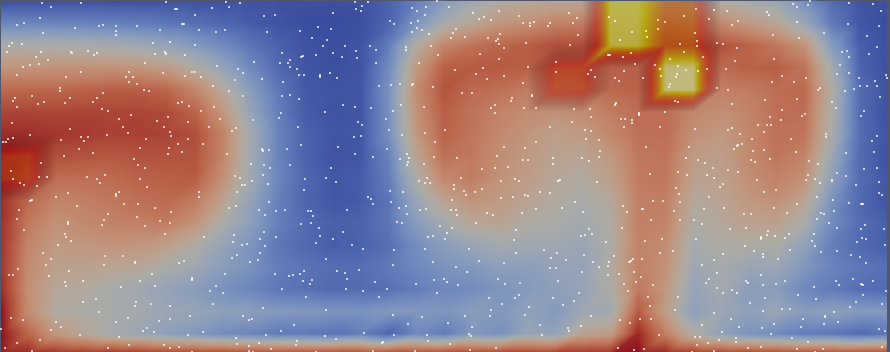
\includegraphics[width=\textwidth]{figures/box_batch38.png}
        \caption{Caption}
        \label{fig:my_label}
    \end{subfigure}
    \hfill
    \begin{subfigure}{0.49\textwidth}
        \centering
        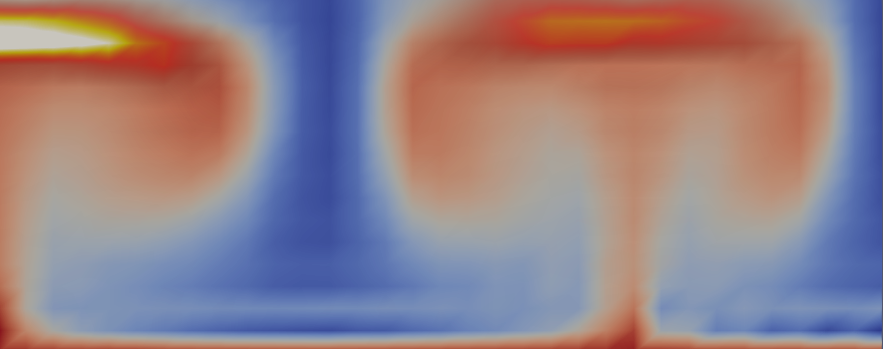
\includegraphics[width=\textwidth]{figures/box_2pp38.png}
        \caption{Caption}
        \label{fig:my_label}
    \end{subfigure}
    %
    \begin{subfigure}{0.49\textwidth}
        \centering
        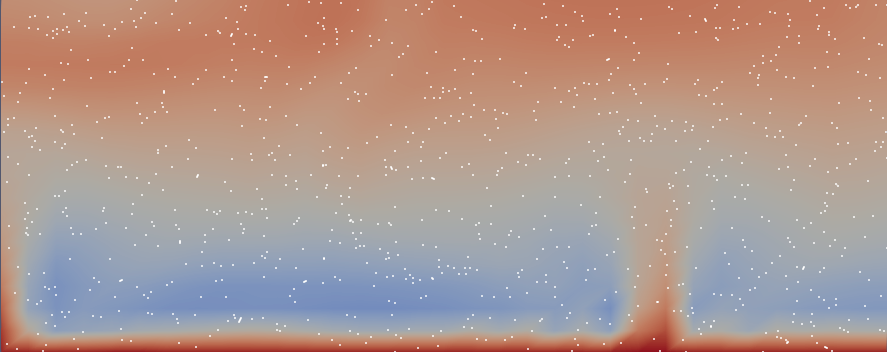
\includegraphics[width=\textwidth]{figures/box_batch79.png}
        \caption{Caption}
        \label{fig:my_label}
    \end{subfigure}
    \hfill
    \begin{subfigure}{0.49\textwidth}
        \centering
        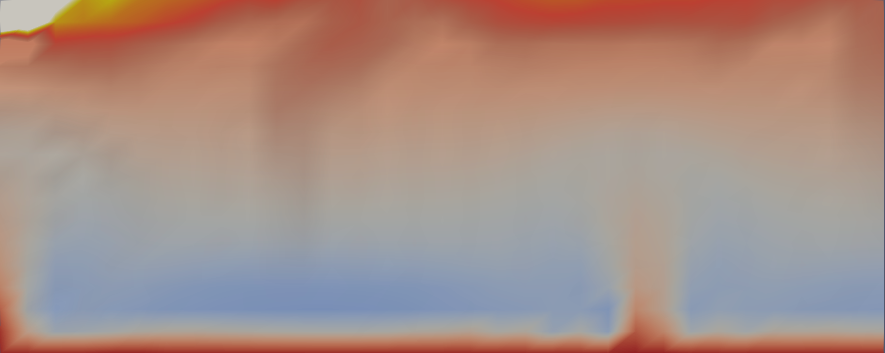
\includegraphics[width=\textwidth]{figures/box_2pp77.png}
        \caption{Caption}
        \label{fig:my_label}
    \end{subfigure}
\end{figure}